\documentclass[english,12pt,a4paper,pdftex]{article}
%\documentclass[english,12pt,a4paper,dvips]{article}

\usepackage[elec,utf8]{aaltothesis}

% pdflatex, gfx in jpg/pdf
\usepackage{graphicx}
%\usepackage{url}
\usepackage[pdfpagemode=None,colorlinks=true,urlcolor=red,%
linkcolor=blue,citecolor=black,pdfstartview=FitH]{hyperref}
\usepackage[comma,sort&compress,numbers]{natbib}

\usepackage{amsfonts,amssymb,amsbsy,amsmath}
\usepackage{tikz}

% flush floats without forcing a partly clear page
\usepackage{afterpage}

% (ugly) euro symbol from €
\usepackage[official]{eurosym}
\DeclareUnicodeCharacter{20AC}{\euro{}}
%or:
%\usepackage{marvosym}
%\DeclareUnicodeCharacter{20AC}{\EUR{}}
\usepackage{textcomp}

% micro sign µ
\usepackage{siunitx}
\sisetup{math-micro=\text{µ},text-micro=µ}

\usepackage{draftwatermark}
\SetWatermarkText{DRAFT}
\SetWatermarkScale{3.33}
%\SetWatermarkColor{gray!20}

\newcommand\bayer[1]{
\begin{tikzpicture}[scale=#1]

% box sizes in screen coordinates; isometric
\newcommand*{\dx}{0.866}
\newcommand*{\dy}{0.5}
\newcommand*{\dz}{0.33}

% ++(a,b) is relative movement from the previous position

% coords for colored or gray top
\newcommand*{\mytopbox}{ -- ++(\dx,\dy) -- ++(\dx,-\dy) -- ++(-\dx,-\dy) -- cycle}
% coords for the left wall
\newcommand*{\myleftbox}{ -- ++(0,-\dz) -- ++(\dx,-\dy) -- ++(0,\dz) -- cycle}
% coords for the right wall
\newcommand*{\myrightbox}{ -- ++(0,-\dz) -- ++(\dx,\dy) -- ++(0,\dz) -- cycle}
% draw the outline first, then the inner edges separately. this prevents
% annoying small ticks in the joined corners where faces overlap. (see the
% tikz manual about the line-to operation's smoothness)
\newcommand*{\myfullbox}[1]{
	(##1)
	% top side clockwise
	-- ++(\dx,\dy) -- ++(\dx,-\dy) -- ++(0,-\dz)
	% bottom
	-- ++(-\dx,-\dy) -- ++(-\dx,\dy) -- ++(0,\dz) -- cycle
	% the inner three: \ | /
	% tikz scale parameter goes bonkers with cycle if first coord is not repeated
	(##1)
	++(0,0) -- ++(\dx,-\dy)
	++(0,0) -- ++(0,-\dz)
	++(0,\dz) -- ++(\dx,\dy)
}

% draw the boxes
\newcommand*{\mybox}[2]{\draw [fill=##1] \myfullbox{##2}}
\newcommand*{\mytop}[2]{\draw [fill=##1] (##2) \mytopbox}
\newcommand*{\leftside}[2]{\draw [fill=##1] (##2) \myleftbox}
\newcommand*{\rightside}[2]{\draw [fill=##1] (##2) \myrightbox}
\newcommand*{\leftcorner}[1]{\draw (##1) ++(0,-\dz) -- ++(0,\dz) -- ++(\dx,\dy)}

\newcommand*{\myboxat}[4]{
	\mybox{##1}{##2*\dx+##3*\dx, -##2*\dy+##3*\dy-##4*\dz};
}
% a row of boxes with row index (incrementing to top right) with y offset
\newcommand*{\rowpartlyq}[4]{
	\foreach \x in {##3} {
		\mytop{##1}{##2*\dx + \x*\dx, -##2*\dy + \x*\dy + ##4};
	}
}
% zero offset rows
\newcommand*{\rowpartly}[3]{
	\rowpartlyq{##1}{##2}{##3}{0}
}
% same row, two different colors and indices
\newcommand*{\rowcolorpair}[5]{
	\rowpartly{##1}{##3}{##4}
	\rowpartly{##2}{##3}{##5}
}
% same row with offset
\newcommand*{\rowbase}[3]{
	\rowpartlyq{##1}{##2}{##3}{-\dz}
}
% row of right sides with an offset
\newcommand*{\rightsides}[4]{
	\foreach \y in {##3} {
		\rightside{##1}{\dx + ##2*\dx + \y*\dx, -\dy - ##2*\dy + \y*\dy + ##4};
	}
}
% alternating colors, zero offset
\newcommand*{\rightsidespair}[5]{
	\rightsides{##1}{##3}{##4}{0}
	\rightsides{##2}{##3}{##5}{0}
}
% row of left sides with an offset, first column for each row
\newcommand*{\leftsides}[3]{
	\foreach \y in {##2} {
		\leftside{##1}{\y*\dx, -\y*\dy + ##3};
	}
}
% alternating colors
\newcommand*{\leftsidespair}[4]{
	\leftsides{##1}{##3}{0}
	\leftsides{##2}{##4}{0}
}

% --- and then the actual rendering
% look at the picture for documentation ;-)
% row lengths: 8 8 8 7 7 6 4 0

% draw order here: 1) floor 2) color tops 3) sides
% three corners are special

\color{black} % line color changeable here

\myboxat{blue}{0}{0}{0}
\rowcolorpair{blue}{green}{0}{2,4,6}{1,3,5,7}

\rowcolorpair{green}{red} {1}{0,2,4,6}{1,3,5,7}

\rowcolorpair{blue}{green}{2}{0,2,4,6}{1,3,5,7}
\rightsidespair{blue}{green}{2}{}{7}

\rowbase{gray}           {3}{7}
\rowcolorpair{green}{red} {3}{0,2,4,6}{1,3,5}

\rowbase{gray}           {4}{7}
\rowcolorpair{blue}{green}{4}{0,2,4,6}{1,3,5}
\rightsidespair{blue}{green}{4}{6}{}

\rowbase{gray}           {5}{6,7}
\rowcolorpair{green}{red} {5}{0,2,4}{1,3,5}
\rightsidespair{green}{red} {5}{4}{5}

\rowbase{gray}           {6}{4,5,6,7}
\rowcolorpair{blue}{green}{6}{0,2}{1,3}

\rightsidespair{blue}{green}{6}{0,2}{1,3}
\myboxat{gray}{7}{7}{1}
\rowbase{gray}           {7}{1,2,...,6}
\myboxat{gray}{7}{0}{1}

% left sides
\leftsidespair{blue}{green}{2,4,6}{1,3,5}
\leftsides{gray}{0,1,...,6}{-\dz}
\rightsides{gray}{7}{1,2,...,6}{-\dz}

\end{tikzpicture}
}

% \simplefig{pos-specifier}{contents}{labelname}{caption}
\newcommand{\simplefig}[4]{%
	\begin{figure}[#1]\begin{center}
		#2
		\caption{#4}
		\label{#3}
	\end{center}\end{figure}
}
% \simplegfx{pos-specifier}{width}{filename-and-labelname}{caption}
\newcommand{\simplegfx}[4]{%
	\simplefig{#1}{\includegraphics[width=#2]{#3}}{fig:#3}{#4}
}

\setlength{\hoffset}{-1in}
\setlength{\oddsidemargin}{35mm}
\setlength{\evensidemargin}{25mm}
\setlength{\textwidth}{15cm}

\setlength{\voffset}{-1in}
\setlength{\headsep}{7mm}
\setlength{\headheight}{1em}
\setlength{\topmargin}{25mm-\headheight-\headsep}
\setlength{\textheight}{23cm}

% \frenchspacing

\graphicspath{ {gfx/tex/}{gfx/dot/}{gfx/bitmap/}{gfx/vector/} }

\begin{document}

\department{Department of Automation and systems technology}%
{Automaatio- ja systeemitekniikan laitos}
\professorship{automagic}{automagia}
\code{AS-1337}

\univdegree{MSc}

\author{Konsta Hölttä}

% a rig for multi-view stereo reconstruction of facial movement
% multi-view stereo image acquisition rig for face reconstruction/content generation
% multi-view stereo reconstruction/acquisition for (realistic) 3d/computer graphics content generation/capture

% multi-view stereo reconstruction for computer graphics content capture
% monen näkymän stereon rekonstruktio tietokonegrafiikan sisällön taltiointiin
\thesistitle{Multi-view stereo reconstruction for computer graphics content capture}{Monen näkymän stereon rekonstruktio tietokonegrafiikan sisällön taltiointiin}

\place{Espoo}
\date{X.Y.2014}

\supervisor{Prof. Ville Kyrki}{Prof.\ Ville Kyrki}
\instructor{Prof. Jaakko Lehtinen}{Prof.\ Jaakko Lehtinen}

\uselogo{aaltoPurple}{!}

\makecoverpage

\keywords{Such words wow}
\begin{abstractpage}[english]
	Very abstract. many wow.
\end{abstractpage}

\newpage

\keywords{Sanoja vau}
\begin{abstractpage}[finnish]
	Tiivistelmä on tiivis.
\end{abstractpage}

\mysection{Preface}
This thesis is the first step in an adventure that started from a need and interest for an end-to-end machinery for acquiring realistic 3D content for computer graphics research and content production in Aalto University.
The work was conducted in the Department of Media Technology at Aalto University, with help from the Automation Technology laboratory.
My personal field of study and greatest interest is Automation and Systems Technology, where similar applications of computer vision can be found in robotics.

I would like to thank my advisor Jaakko Lehtinen for his guidance regarding this work and for the glorious opportunity to work on such an interesting subject, and my supervisor Ville Kyrki for valuable and supportive feedback on this thesis.
Thanks too to my co-workers at the time, Markus Kettunen, Miika Aittala and Ari Silvennoinen, for inspiring discussions about computer graphics during this work.

Last but not least, thanks also to my family and friends for all the help and support.
Of them, special greetings to Arto Rusanen and Samuli Vuorinen for sharing their deep knowledge in imaging technology and lending me photography hardware.
Arto also kindly worked as a test subject.

\vspace{5cm}
Otaniemi, dd.mm.2015

\vspace{5mm}
{\hfill Konsta ``sooda'' K.\ Hölttä \hspace{1cm}}

\newpage

\thesistableofcontents

\mysection{Symbols and abbreviations}

\subsection*{Symbols}

\begin{tabular}{ll}
$M$	& Capital letters are matrices\\
$\vec v$	& lowercase letters with arrows on top are vectors\\
$\vec v_i$	& $i$th 
\end{tabular}


\subsection*{Operators}

\begin{tabular}{ll}
$\sum_i $                        & sum over all indices $i$\\
$\mathbf{a} \cdot \mathbf{b}$    & Dot product of the vectors $\mathbf{a}$ and $\mathbf{b}$
\end{tabular}

\subsection*{Abbreviations}

(should these be explained in short or not?)

\begin{tabular}{ll}
	2D & two-dimensional\\
	3D & three-dimensional\\
	SIFT & Scale-invariant feature transform\\
	SURF & Speeded up robust features \\
	PCL & Point cloud library\\
	OpenGL & Open graphics library, a well-known standard API for rendering 3D and 2D graphics\\
	mocap & motion capture, the procedure for acquiring 3D motion in digital form\\
	CCD & Charge-coupled Device\\
	CMOS & Complementary Metal-Oxide Semiconductor\\
	SLR & Single-lens reflex camera\\
	DSLR & Digital SLR\\
	FPS & Frames per second\\
	SW & Software\\
	HW & Hardware\\
	API & Application Programming Interface\\
	CG & Computer Graphics\\
	SfM & Structure from Motion\\
\end{tabular}



\cleardoublepage
\storeinipagenumber
\pagenumbering{arabic}
\setcounter{page}{1}

% Johdanto
\section{Introduction}

%% Leave first page empty
% (wat?)
\thispagestyle{empty}
History[edit]

One of the first papers discussing performance-driven animation was published by Lance Williams in 1990. There, he describes 'a means of acquiring the expressions of realfaces, and applying them to computer-generated faces'.[1]
%%http://en.wikipedia.org/wiki/Facial_motion_capture
% subsect intro, subsect overview?
HOX shorten this section and move some of this to the background section.

Computer vision is a mature field; the steps of acquiring three-dimensional structure of a real-life scene are well known.
Stereo, multiview, structure from motion, blah blah.

This work concentrates most on scanning human faces, but the algorithms are kept as abstract as possible to make it simple to apply them to other targets too.
Acquiring structure of static objects is also presented.

Facial motion capture (mocap) is currently a standard tool in the movie and video game entertainment industry among the more mature mocap for whole body movement.
Mocap records movements of a human body (or another object tjat is to be recorded) so that the movements can be replayed or analyzed.
Level of detail varies depending on what is needed; from simple bone movements to deformations of skin and muscles.
Usually the capture is done on special easily distinguishable markers, typically small retroreflective dots, that are mapped to a model for playback. Playback then interpolates between the recorded positions. [CITE THESE]
% http://www.siggraph.org/education/materials/HyperGraph/animation/character_animation/motion_capture/history1.htm

The Matrix (1999) \cite{wachowski99matrix}, famous of the bullet-time scenes, used heavy optical flow processing to ``slow time down''; The Matrix Reloaded \cite{wachowski03reloaded} used a technique called Universal Capture by Borshukov et al. \cite{borshukov05universal}.
(Other applications (uses). Movies. Remedy? Medical [essential physics of, bushberg]!). Landscape/architecture engineering. Crime scenes (police investigation). Topographic mapping. Geology, archaeology. Object replication with 3d printing. Aerial photography (digital elevation models DEM)
Close range photogrammetry

Three-dimensional capture means in general the way of recording a sequence of movements of a real-life target or scene.
The technical details vary by what information is required and available.

Static capture is simple in the way that the time when the pictures are taken does not affect the performance.
Small objects have been scanned successfully with a turntable [CITE], and structure from motion techniques have recently been presented that impressively recover a structure from pictures taken all over an outdoor location with no a priori information about the camera configurations [CITE].

The movie industry usually knows the structure of the objects that are tracked; a pre-recorded mesh is used as a helping model (also called ``virtual bones'' [CITE] universal capture) to track the object pose [CITE].
It is obviously easier to map image features to a priori information than to recover a fully unknown structure.
(A pre-recorded higher resolution texture could be used for pore-level details, then tracking with a good-enough resolution and possibly markers to get wrinkles.)

The intention of this work is both capturing the structure and texture of a target and tracking of the target's movement by time.
The captured data should then be used to reconstruct the same target.
A camera rig is constructed to record continuous video from several, carefully decided viewpoints.
In addition to multiple cameras at different locations and poses, an uniform lightning is also required to minimize specular difficulties in the texture.

The structure of an object can be extracted relatively easily from distinct features that can be detected with several cameras [CITE].
Current advances in camera technology and price make it possible for consumers to do pretty sophisticated reconstruction that has been possible only with a large budget of e.g. a movie studio.
Even software that uses only a smart phone camera and runs on the same phone has been published [CITE, CITE].

The objective of this work is to describe a complete 3D object scanning and reconstruction pipeline with both shape and texture information.
A rig of cameras is constructed, and a generic software pipeline is developed and presented, for reading generic video stream and producing raw reconstructed textured 3D meshes and/or point clouds for further handling.
Real-time processing is not considered important, as the data will be post-processed and observed manually and not used as such.

The reconstruction and rendering involves lots of filtering of the raw data and further using high-resolution textures to extract better resolution depth data than what is available with computer vision technologies only.
By making certain assumptions on the texture, very detailed bump maps can be extracted, for example, by backprojecting the expected 3d mesh to textures and refining. [CITE]

Reconstruction of a static detailed mesh is difficult enough; human faces not only move, but also deform very heavily, which poses even further challenges [CITE].
We present basic techniques for taking also motion into account, but leave the use of state-of-the-art algorithms for future implementations.
It is possible to assume locally smooth movements in most areas; thus, a more intelligent approach should be used than simply reconstructing a new mesh for each frame and using registration to just align them. [CITE]

Many tracking algorithms work in the 2D space using simply the picture data and not the post-processed 3D meshes [CITE].



%snake surrounding stuff

%visual hull

%NASA cams

% Aikaisempi tutkimus
\section{Image acquisition} \label{sec:image-acquisition}

% TODO: image of a scene, a camera with optics and sensor, and a computer, all connected

% tell also briefly what calibration is

%Digital stereo vision analyses digital images for depth cues.
%A digital photograph is variations in light intensity on an image sensor that have been digitized.
%In front of a sensor is a lens system that projects an image to the sensor.

Stereo vision works by analyzing images for depth cues.
It is important that the images are sharp and noise-free.
This section describes the background theory for basic image acquisition steps in a camera and main concerns that affect reconstruction quality.
Steps in an image acquisition pipeline in a single camera are depicted in Figure \ref{fig:camerapipeline}; remarkable steps are described in this section.
Reconstruction accuracy depends on not only measureable parameters of a stereo imaging rig, such as camera positioning accuracy, but also on e.g. lens imperfections, camera focus, camera sensor noise, image compression and algorithmic accuracy. \cite{hollsten2013imagequality,kyto2011method,rieke2009evaluation}.

\simplegfx{h}{0.7\textwidth}{camerapipeline}{
	Image acquisition pipeline in a typical modern camera consists of several optical and digital steps with additional post-processing.
	Image from \cite[p.\ 74]{szeliski10vision}.
}


\subsection{Imaging} \label{sec:imaging} % {{{

From the perspective of this thesis, images are taken with digital cameras that project a three-dimensional view from a single viewpoint to an image plane and store the resulting data in digital form.
This section describes the process of capturing a still photograph.

In the digital world, images are stored and presented as \emph{arrays of numbers}, in discrete form, as opposed to the continuous data in the real world.
A rectangular \emph{raster image} consists of a regular grid of picture elements, or \emph{pixels}.
Each pixel represents light intensity and color at a point.
A digital camera has the same optical working principles as an analog film camera;
the main differences are in image storage as a discrete array of pixels and acquisition using a \emph{sensor}, as opposed to a photosensitive film.
Typically, color pictures are described with separate intensity channels, in e.g.\ Red-Green-Blue (RGB) space, as human vision is also trichromatic.
A single RGB color encodes the intensities of the three primary colors (red, green and blue) separately.
%digital images are only described as a discrete grid of numerical values that describe light intensities, whereas analog film .

Reconstruction algorithms assume a \emph{pinhole camera} model on the camera optics, and the images must be captured such that the model is accurate.
However, as is described in this section, cameras in reality seldom match the simplified model thoroughly, and care must be taken when configuring the cameras and post-processing the images later.
%Lens systems are configured such that the subject is in focus, and optical distortions are corrected.

% }}} imaging

\subsubsection{Pinhole camera} \label{sec:pinhole} % {{{

%near objects look bigger than distant objects

% What's a pinhole camera, what projection means.

\simplegfx{h}{0.6\textwidth}{pinhole-camera}{
	Pinhole camera principle.
	The box represents a camera.
	Image seen through the small hole is formed to the plane on the back of the box, rotated upside down, as rays of light travel from the subject through the hole.
}

A physical camera is in its simplest form modeled as a \emph{pinhole camera}; an ideal device that \emph{projects} an image on its film through an infinitesimal aperture, rotated 180 degrees around the \emph{optical axis}, i.e.\ the line that runs through the pinhole and is perpendicular to the image plane.
Illustration of the process is given in Figure \ref{fig:pinhole-camera}; for example, light rays from the top right of the subject travel through the pinhole to the bottom left on the film.
The term \emph{projection} means the representation of three-dimensional objects on a flat surface, seen from a single point such as the human eye.
The \emph{perspective projection} effect makes objects further away from the observer look smaller in the projected image.
A cube projected on a plane is shown in Figure \ref{fig:perspproj}.

In the scope of this thesis, the only actual camera type considered is one with a \emph{rectilinear lens}; that is, an optic system that preserves straight lines, as a perspective projection does in a pinhole camera.
More exotic lenses that have a completely different projection are not considered, such as ``fisheye'' lenses, although their projections can be corrected in software.

\simplegfx{h}{0.5\textwidth}{perspproj}{
	Perspective projection: a cube seen from a camera at origin O.
	For example, the 3D point $P$ projects on to $p$ on the green plane.
	In a camera, the rays of light travel through a common point to the film that is behind the origin; a virtual projection film between the origin and the object is often used for simplicity.
	Parallel lines in 3D connect in \emph{vanishing points}, two drawn in the left and right.
}

% http://en.wikipedia.org/wiki/Perspective_projection rays of light etc.

% Cartesian coordinates.

Mathematically, a point in a three-dimensional world can be encoded in any coordinate system;
in this work, a standard 3D cartesian coordinate system is used.
In cartesian coordinates, a point is described as a location relative to a selected origin reference, as a triplet of distances along three perpendicular X, Y and Z axes. % (Figure \ref{fig:coordsys}).
In a traditional right-handed system, X increases right, Y upwards and Z towards the viewer.

%\simplegfx{h}{0.6\textwidth}{coordsys}
%{A 3D cartesian coordinate system. Origin at O, point location encoded in the triplet $(x,y,z)$ as individual lengths along the X, Y and Z axes, respectively.}

% }}} pinhole

\subsubsection{Optics} % {{{

% XXX szeliski here

%Practical algorithms take lens imperfections into account (e.g. \cite{opencv}).

In practice, no actual camera works ideally; a pinhole-resembling camera with a tiny hole could be built, but it would have poor light gathering power and low resolution limited by diffraction effects. \cite{todo}
Light sensitivity is increased by using a larger hole, and the light rays are directed using carefully manufactured lens systems.
Refraction properties of light rays and manufacturing defects introduce additional distortions that must be taken into account.
%In practice, lens distortions deviate the rays nonlinearly, and no system is in perfect focus, so that one point spreads out as a circle.

Construction of optical systems is well studied. \cite{kingslake1989history,greenleaf1950photographic}
Actual camera ``lenses'' (\emph{camera objectives}) consist of not only a single glass element (optical lens) but many, especially in the case of zoom lenses.
%where the focal length can be changed.
As an example, a mechanically simple fixed focal length Canon lens diagram is shown in Figure \ref{fig:canonef50mm}.
There are several lenses, aligned so that their centers lie on the the optical axis parallel to it.
Most objectives can be reduced to a \emph{thin lens} model (depicted in Figure \ref{fig:thinlens}), an ideal optical model of a single infinitesimally thin glass element.
% XXX Some lenses implement optical stabilization as a moving element in the light path.

\simplefig{t}{%
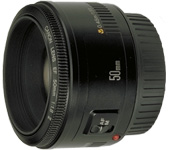
\includegraphics[width=0.4\textwidth]{canonef50mm-1}
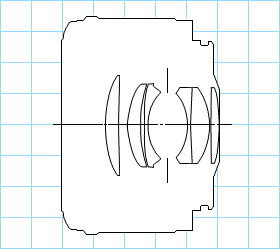
\includegraphics[width=0.4\textwidth]{canonef50mm-2}
}{fig:canonef50mm}{
	A fixed focal length Canon EF 50mm f/1.8 II camera objective.
	Left: the device, not attached to a camera.
	Right: block diagram of the lens construction, showing the six optical elements.
	Diagram by Canon Camera Museum.
}


\simplefig{t}{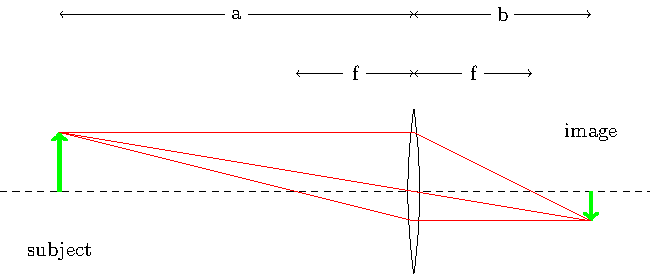
\includegraphics{lens}}{fig:thinlens}{
	thin lens sample: $a=6$, $b=3$, $f=2$.
	Actual subjects would be usually much further away; image depicts a macro setup for clarity.
	A subject at a distance $a$ is \emph{focused} on a film at a distance $b$ on the other side.
}

\paragraph{Focusing}
A subject is said to be \emph{in focus} when the light rays originating from it converge at the same point on the camera's film.
When the camera objective is adjusted for the object to be in focus, its parameters are changed slightly and a different thin lens is formed.
\emph{Focal length} is a fundamental property of a lens and determines its amount of magnification.
Illustrated in Figure \ref{fig:thinlens}, the thin lens model and its focal length $f$ encode a relation between an object at a distance $a$ and its \emph{focused} image at a distance $b$ on the other side, as shown in Equation \ref{eq:thinlens}.
A camera system typically has a \emph{magnification} of much less than one; i.e.\ the image on its film is rendered smaller than the imaged subject, as $a >> b$.
%For a lens focused at \emph{infinity} ($a = \inf$), $b$ becomes equal to $f$ and a pinhole model becomes accurate.
For objects at distances approaching infinity ($a = \inf$), $b$ becomes equal to $f$, and the thin lens resembles a pinhole with film distance $f$. \cite{szeliski10vision}

\begin{equation} \label{eq:thinlens}
	\frac{1}{a} + \frac{1}{b} = \frac{1}{f}
\end{equation}


% http://www.canon.com/camera-museum/lens/ef/data/standard/ef_50_18ii.html?p=2

%The focal length has a direct influence to field of view, as given in figure TODO. Longer focal length (long-focus lens, often referred to as telephoto lens) results to a more zoomed in picture, as opposed to a wide-angle lens. 

% Aperture.

\paragraph{Aperture}
The size of the hole where light effectively goes through is called \emph{aperture}; the hole itself is called \emph{aperture stop} and it is located inside the the objective in between its lenses.
The diameter of a thin lens corresponds to the aperture diameter and to the stop's \emph{entrance pupil}, the aperture stop seen from the front of the objective.
As in any practical case, it is not infinitesimally small, and there will be some area of the scene that is imaged as sharp and others in front and behind of this area will be blurred.
This effect is called \emph{depth of field (DOF)} and is illustrated in figure \ref{fig:irldof}.
In artistic photos, a \emph{shallow} depth of field can be preferred; having the subject in focus separating separate it from the background by blurring the background.
In 3D reconstruction, exactly the opposite is preferred: everything should be sharp, in deep focus.
The aperture size is presented as relative to the focal length and is commonly called the \emph{F number} \cite{szeliski10vision}, specified via the aperture diameter $d$:

\begin{equation} \label{eq:fnumber}
	N = \frac{f}{d}
\end{equation}

\simplefig{b}{%
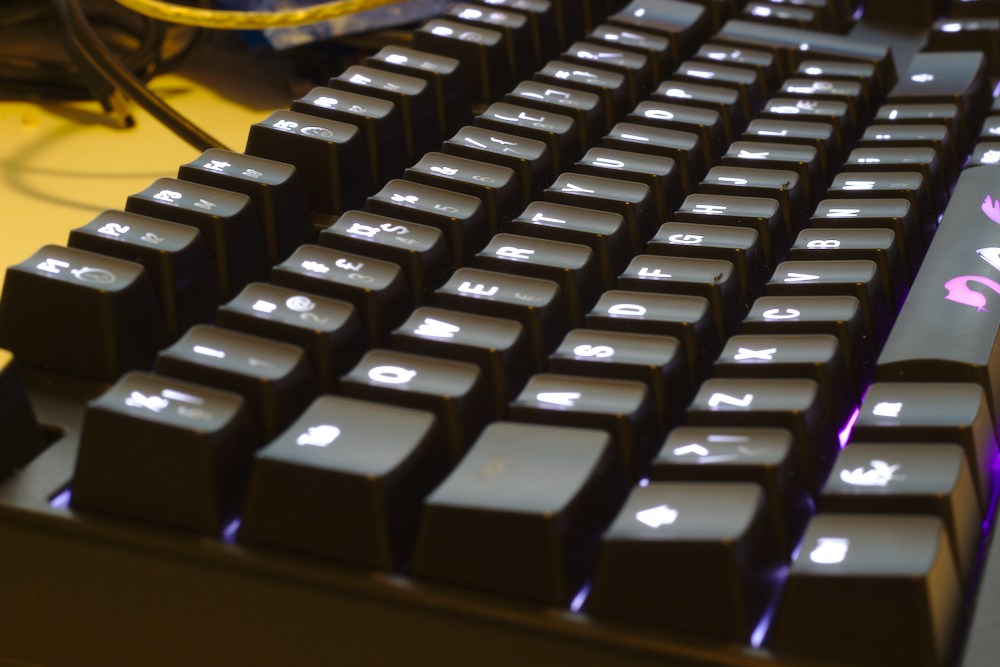
\includegraphics[width=0.45\textwidth]{irldofdeep}
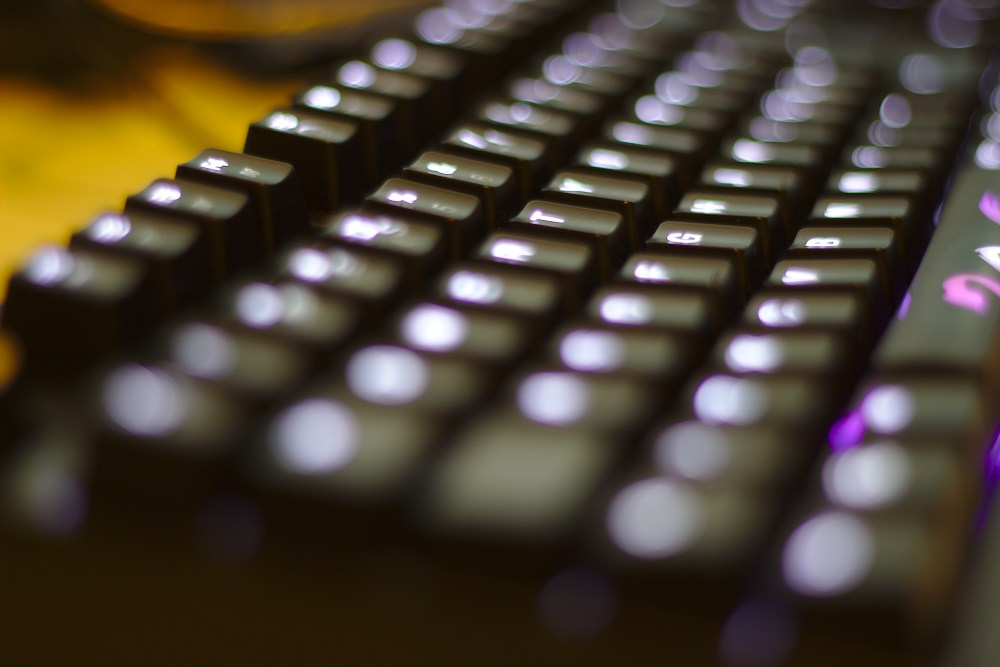
\includegraphics[width=0.45\textwidth]{irldofshallow}
}{fig:irldof}{
	Deep and shallow depth of field in close-up photography using a 50 mm lens.
	Left: F/16 aperture, 15 second exposure, showing only slight blur in the nearest keys.
	Right: F/1.8, 0.2 s exposure, with only a small sharp area.
	The image blurs and the distinctively brighter lit markings on the keys show as increasingly larger bright spots as the circle of confusion increases.
}


Doubling the area of the aperture equals to an increase of the diameter $d$ by $\sqrt 2 \approx 1.4$.
The aperture size is typically denoted as $f/\#$, where $\#$ is replaced by the number, such as $f/1$ or $f/1.4$.
This makes the amount of light reaching the film universal among all focal lengths.
Full multiples of $\sqrt 2$ are called \emph{stops}.
\cite{szeliski10vision}

\paragraph{Circle of confusion}
As the blur happens gradually, the ``level of sharpness'' at each point is often defined via a \emph{circle of confusion} (CoC).
The distance from the lens along the optical axis where perfect focus is attained is called the \emph{focal plane}.
Every point nearer or further away shows up on the film as a circle (for circular apertures); when this circle is significantly larger than the resolving power of the observer, the image of this point is perceived as blurred.

Depth of field is defined as difference between the shortest and farthest object distances that still generate an acceptable CoC, found geometrically.
When $f$ is the focal length, $N$ the aperture f number, $s$ the distance to the subject, and $c$ the maximum acceptable CoC, the depth of field $D$ is given by (from \cite{greenleaf1950photographic}):

\begin{equation} \label{eq:dof}
	D = \frac{2 s f^2 N c (s - f)} {f^4 - N^2 c^2 (s - f)^2}
\end{equation}

\simplegfx{h}{\textwidth}{dofcoc}{
	Exaggerated illustration of depth of field and circle of confusion with a thin lens, seen from the side (not drawn to scale).
	Subjects at distance $s$ project perfectly at the film.
	Distances between $Z$ and $Z'$ project to a circle smaller or equal to $c$.
	It can be easily seen that for subjects at longer distances, the depth of field increases.
}


In Figure \ref{fig:dofcoc}, $Z'$ and $Z$ are the maximum and minimum acceptable distances near the subject, and $Z' - Z = D$.
Sufficient depth of field is important to consider in near-field 3D scans, which translates to a small aperture, and consequently, really bright lights.
The subject should fill whole image frame to use the pixel density effectively.
Increasing the distance to the subject would increase depth of field, but enlarging the subject in the frame again would need a longer lens, which decreases depth of field.

Acceptable size of the CoC depends on the resolving power of the viewer; when a photograph is looked with the eye, the print size of the image determines the circle.
A standard-considered formula in photography determines the maximum acceptable CoC by dividing the image size by 1500, originating from human eye and viewing distance.
For the standard ``full-frame'' 35 mm film size with an image size of 36 x 24 mm (approx.\ 43 mm diagonal), the CoC becomes $c = 43 \text{ mm} / 1500 \approx 0.03 \text{ mm}$.
In reality, an intuitive way to determine the disk size is the size of a single pixel in a digital sensor replacing the film;
the disk should not span too many pixels, so that accurate detail would be resolvable from the digital image.
For a normal 50 mm lens with the subject at a distance of 1 m, an aperture of f/11 and a circle of confusion of 0.03 mm, the formula \ref{eq:dof} gives $D \approx 25 \text{cm}$. % , having the subject approximately in the middle of the acceptable range.

% diffraction

\paragraph{Diffraction}
The required amount of light is not the only factor that limits the minimum aperture size.
\emph{Diffraction} is an effect that blurs the image with too \emph{small} apertures.
When light rays diverge on a small aperture, their different distances traveled make the waves interfere each other and produce a two-dimensional diffraction pattern, called an \emph{airy disk}, named by  George Biddell Airy.
The disk blurs the image in a similar fashion as an object that is out of focus.
Size of the airy disk is relative to the size of the aperture and the light wavelength.
Thus, the aperture size must be set to a balance between the unwanted effects of DOF and diffraction.
The disk size can be approximated by

\begin{equation} \label{eq:airydisk}
	x = 1.22 \frac{\lambda f}{d} = 1.22 \lambda N
\end{equation}


which, for red light in the visible spectrum having a wavelength $\lambda$ of 700 nanometers, with an aperture of f/11, results in $\approx$ 0.01 mm (compare to above CoC of 0.03 mm).
\cite{greenleaf1950photographic}

% rayleigh limit?

% XXX TODO linear projection: straight lines in the world map to straight lines in the image (p. 58)

\paragraph{Geometric distortion}
While most rectilinear lenses are close to a perspective projection, practical optical systems introduce some non-linear \emph{radial} and \emph{tangential distortion} that affect the accuracy of the ideal pinhole model.
Common distortions are the purely radial so-called \emph{barrel} and \emph{pincushion} distortions, where the lens magnification is a nonlinear function of image ray distance from the center of the lens, caused by the shape of the lenses. \cite{brown1966decentering}
In addition to radial, tangential distortion is less significant, and it is often ignored.
Its cause is small misalignments in separate elements in a single optical system; lenses being offset from each other and not being parallel to the image plane. \cite{kingslake1989history}

%Wilson \cite{wilson2004anton} discusses optical systems' relation to depth of field, focus and distortions.

\simplefig{h}{%
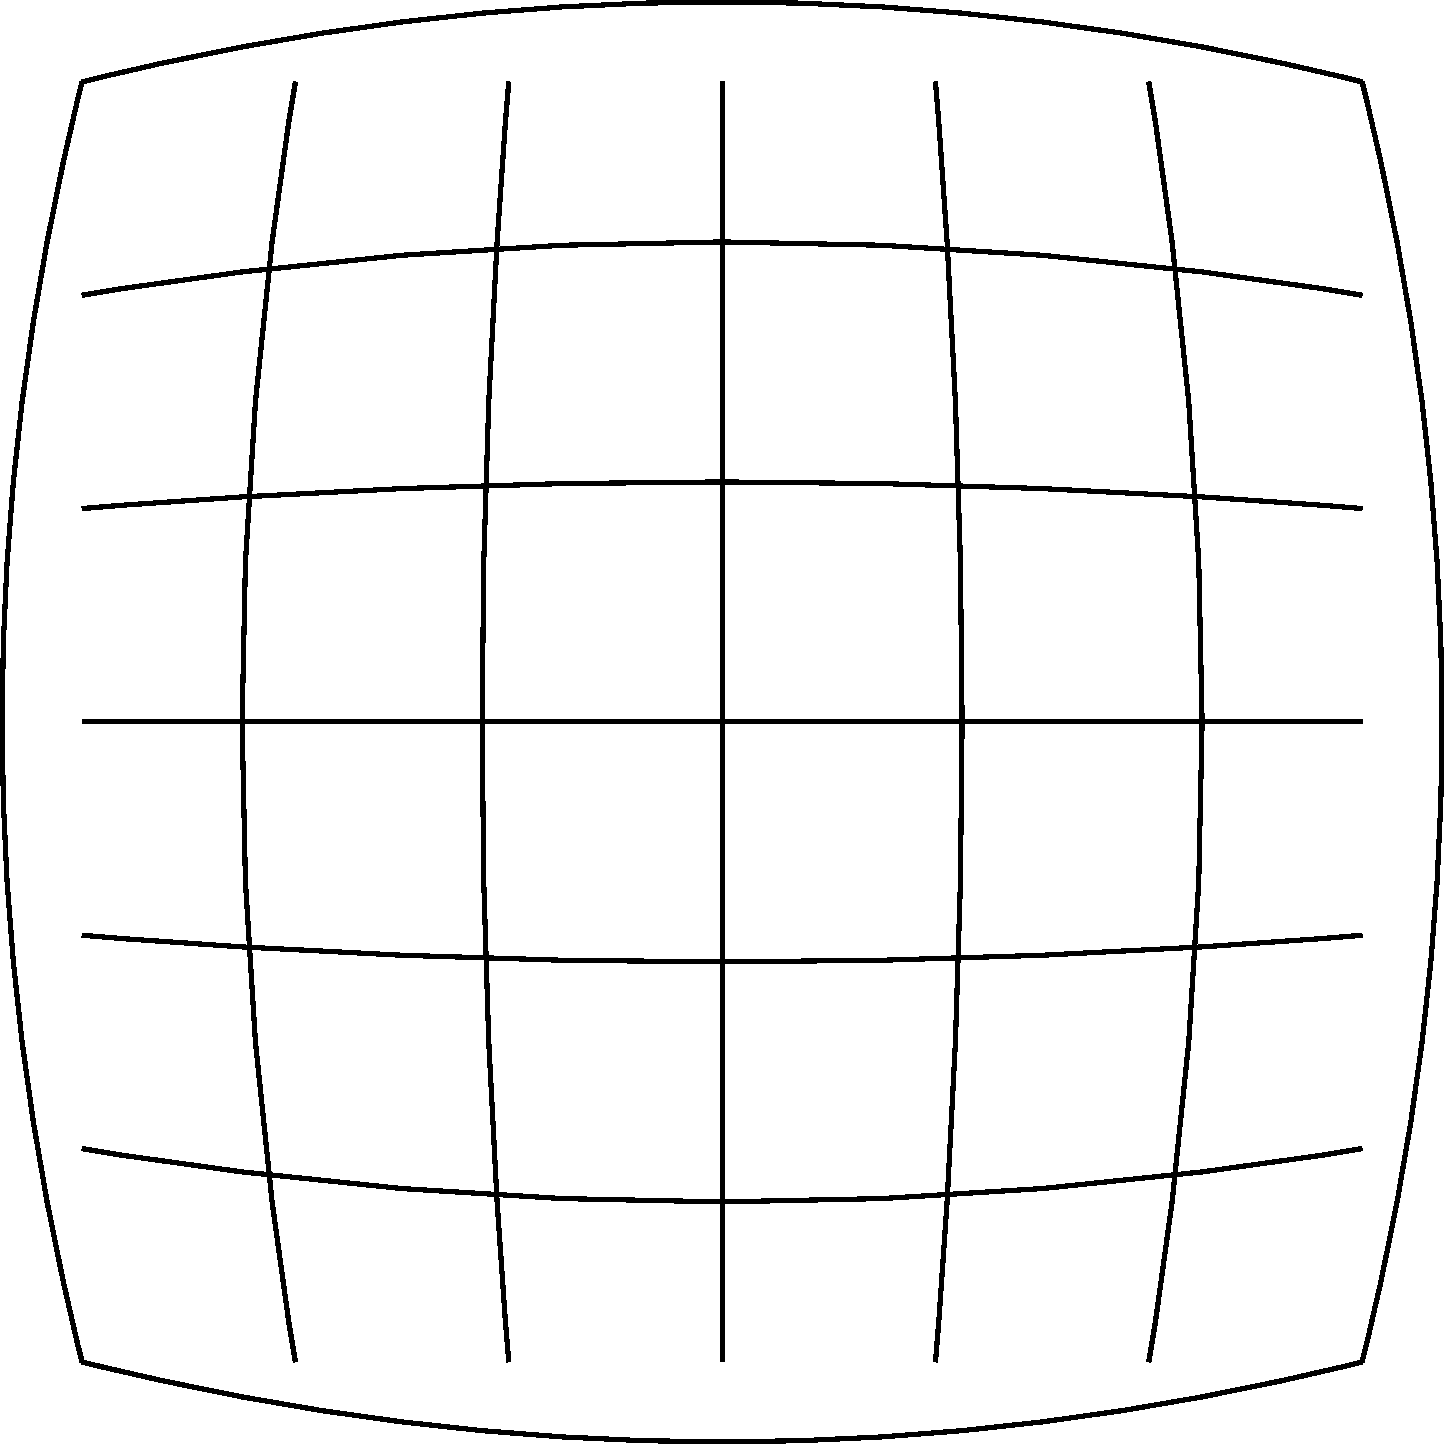
\includegraphics[width=0.2\textwidth]{barrel-distortion}
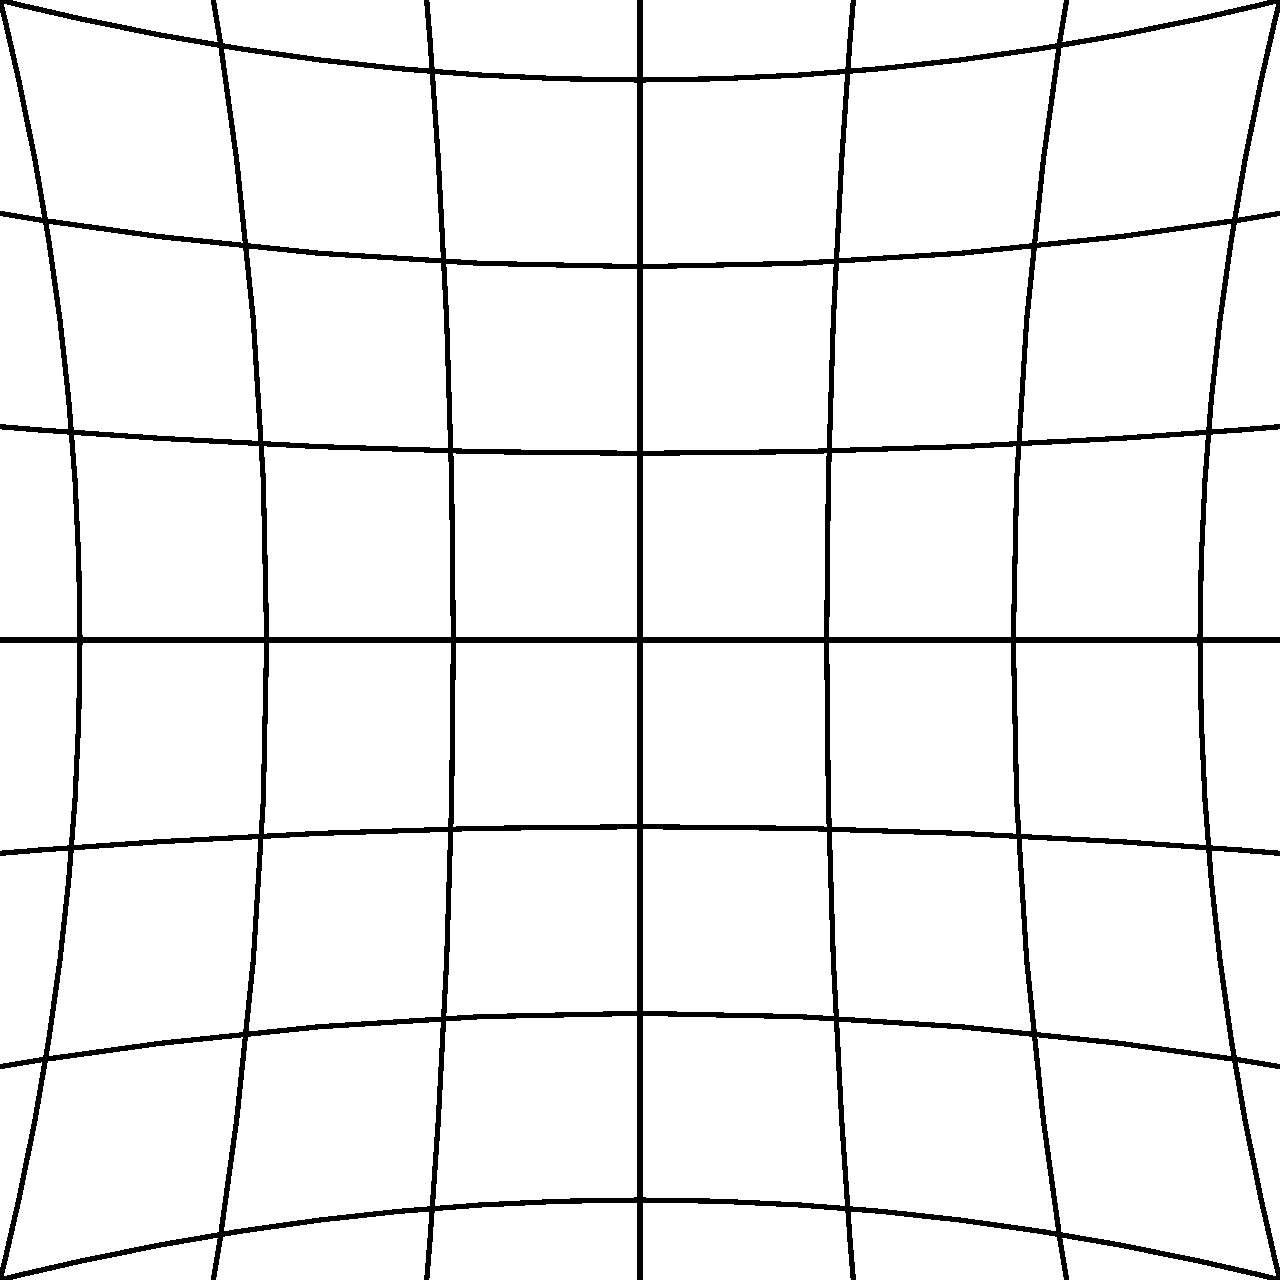
\includegraphics[width=0.2\textwidth]{pincushion-distortion}
}{fig:distortions}{
	Barrel (left) and pincushion distortions that would show up in an image of a grid of straight lines.
	For a lens with no distortion, the lines would not be curved but in a perfect grid.
}

Geometric distortion must be corrected in software, because stereo vision algorithms assume that the images are free of nonlinear errors, i.e. straight lines in the world should remain straight in 2D images after the projective transformation.
%In particular, image rectification (discussed later in \ref{sec:rectification} won't work if this straightness does not remain; the assumption that similar features should be found on horizontal lines wouldn't hold on distorted images. \cite{hartley03multiview} 

The radial error model and correction proposed first by Brown \cite{brown1966decentering} and used by e.g. the OpenCV library \cite{opencv} is % to create a new image of the original pixel values at new positions is

\begin{align} \label{equ:radialdist} \begin{split}
	x_{corr} &= x(1 + k_1 r^2 + k_2 r^4 + k_3 r^6)\\
	y_{corr} &= y(1 + k_1 r^2 + k_2 r^4 + k_3 r^6)
\end{split} \end{align}

% (XXX some software does this in a different way (inverse of this, maybe?)

Trucco and Verri \cite{trucco1998introductory} use only the two first coefficients, and some use only the first $k_1$; for lenses with low distortion, this is often enough.
For tangential distortion, the corresponding correction has the following form:

\begin{align} \label{equ:tangdist} \begin{split}
x_{corr} &= x + (2 p_1 x y + p_2 (r^2 + 2 x^2))\\
y_{corr} &= y + (2 p_2 x y + p_1 (r^2 + 2 y^2))
\end{split} \end{align}

In eq. \ref{equ:radialdist} and \ref{equ:tangdist}, $x$ and $y$ are the original coordinates in the distorted image, $x_{corr}$ and $y_{corr}$ are the corrected ones, $k_1$, $k_2$, $k_3$, $p_1$ and $p_2$ are coefficients specific to the distortion, and $r$ equals to the distance to image center where the optical axis lies, located at $(x_c,~y_c)$:

\begin{equation}
r = \sqrt{(x - x_c)^2 + (y - y_c)^2}
\end{equation}


The image size is normalized such that the coordinates $x$ and $y$ range from $-1$ to $1$, making the distortion parameters universal for all image resolutions.
The effects of different parameters are depicted in Figure \ref{fig:raddist}.
% TODO: only first and also ka and kb for comparison

\simplegfx{h}{\textwidth}{raddist}{
	Barrel-type radial distortion with different parameters.
	Lines point from destination image pixels to locations to sample from in original image.
	Left: $k_a = 0.16$, middle: $k_b = 0.08$, right: $k_a = -0.04, k_b = -0.04$.
}

% XXX HOXHOX THIS SOMEWHERE TODO BEGINNING
Because digital images consist of a discrete pixel array, the pixel coordinates given by the undistortion do not necessarily lie on exact pixel positions; the sampling should then interpolate between neighboring pixels, instead of taking the nearest color. \cite{wolberg1990digital}

%Perspective distortion something something viewer location.
%Normal TV is usually watched at the distance of twice the screen diagonal.
%At this location, the scene looks normal when taken with a normal lens.
%A wide-angle scene then looks normal when viewed at a nearer distance. \cite{wilson2004anton}

% 14:01:55 <naavis> Kai sillä yritetään emuloida sitä, että katsojan paikalta se leffan kuvakenttä vastais sitä että valkokankaan tilalla on ikkuna.

% }}} optics

\subsubsection{Shutter} % {{{

% shutter, why needed

A static scene is imaged by exposing the photosensitive film (or sensor) to the light passing through the optics for a short time, keeping the camera and subject steady.
A \emph{mechanical shutter} blocks the light before and after the exposure.
In recent digital image sensors, the sensor itself can be made inactive to light or cleared quickly from the accumulated charge; this is called \emph{electronic shutter}.
%Electrical sensors can be cleared to black rather quickly.
%Still, good quality cameras use even faster mechanical shutters for photographs.
%Because of the rolling shutter effect of a CMOS sensor, it is better to do the reset and readout phases when the sensor is not exposed to light.

% mechanical stuff

\simplegfx{h}{0.6\textwidth}{focalplaneshutter}{
	Focal plane shutter has two moving curtains to cover the film, opening it momentarily so that each part of the film receives light for the same amount of time.
	From left to right: initially, the film is blocked.
	Once the first (shown in red) curtain moves away, the film is exposed to light.
	A second curtain (shown in blue) stops the light from entering again.
	The shutter resets by moving back to the initial position.
}

\simplegfx{h}{0.6\textwidth}{focalplanerolling}{
	Rolling shutter effect in a focal plane shutter happens when the exposure time is really short.
	The shutters have to move at the same time, exposing only a part of the film at a time.
	Fast movement during the exposure leads to artifacts and a short flash light would illuminate only a part of the film.
}


\paragraph{Shutter types}
All shutters serve the same purpose: to restrict the light from entering the image plane before and after the exposure.
%A shutter is a mechanical device that blocks light to the film and can be moved momentarily out of the way and back.
There are several types of constructions for shutters, depending on the application.
Some cheaper compact cameras have a small \emph{leaf shutter} in the lens center near the aperture stop.
A leaf shutter moves quickly away from the light path and back, either as a single opaque piece or as several \emph{leaves}, analogously to the aperture stop.

A \emph{focal plane shutter}, used in most system cameras, is installed in front of the film plane.
Leaf shutters would be expensive to install in each interchangeable lens, and a focal plane shutter can operate at higher speeds.
Focal plane shutter consists of two curtains that move to the same direction; one moves out of the way of the film to let light pass to it, and another moves to cover it back again when the exposure time has elapsed.
Figure \ref{fig:focalplaneshutter} illustrates the working principle of a planar shutter.
In film cameras, the focal plane shutter was originally two fabric ``curtains'';
today, they are constructed from small, interleaved metal or plastic sheets.

Some cameras have only an \emph{electronic shutter} instead of moving parts.
Electronic image sensors cannot only be cleared and read out at a restricted rate, which is why they have some defects.

Video film cameras that capture each frame to a separate part of film used a spinning wheel with a transparent window, called rotary disc shutter. \cite{wilson2004anton}
This rotates at a precise speed synchronized to the frame rate, displaying a for a consistent duration for each frame.
The size of the window constitutes to the amount of light and motion blur.
Video is more discussed in the section \ref{sec:video}.

\paragraph{Artifacts}
If the camera or the imaged subject moves while exposing the frame, the subject gets smeared along the movement on the image, an effect known as \emph{motion blur}.
A related \emph{rolling shutter} effect is produced using a focal plane shutter with very high speeds, where the limit of curtain speed prohibits fully opened shutter.
The closing curtain starts to move before the first has stopped, exposing only a narrow band of the film at a time.
Fast mechanical shutter movement is depicted in Figure \ref{fig:focalplanerolling}.
When an object is moving to the same direction as the narrow shutter slit, i.e. vertically, it appears smeared;
when the movement is horizontal, different parts of the subject appear to bend.
An electronic flash light also cannot be used with high focal plane shutter speeds, as it would illuminate only a narrow slit of the sensor.
Electronic shutters also suffer from a similar effect; this is more discussed in section \ref{sec:sensors}.
Since a leaf shutter opens radially, it does not have this effect, and it can be used at higher speeds with flash lights.
Leaf shutters suffer from another artifact:
at higher speeds, the longer time spent covering the far sides of the image can lead to uneven brightness.
%Result of shooting a moving object with rolling shutter is depicted in figure \ref{fig:rollingeffect}.

%\simplegfx{h!}{0.8\textwidth}{fig:rollingeffect}{
%	Rolling shutter imaging a spinning disk.
%	At each point in time, the slit captures only part of the subject.
%	When the object moves, the subject appears distorted.
%	Image by Wikipedia user Cmglee, licensed under CC BY-SA.
%}

%A digital CMOS exposure and ``electrical shutter'' works like this too; the sensor is reset and read row by row sequentially; this produces a strong rolling shutter effect especially in video cameras when the subject is moving fast relative to the camera.
%
%A CCD camera would not need a mechanical shutter, because the full image is read out at once.
%Most still cameras have also a movie mode that holds the mechanical shutter open all the time, using the electrical shutter.
%
%The mechanical shutter can last only a finite amount of actuations (50 000-200 000 for a common system camera) as it wears out gradually.

% other

\paragraph{Lag}
When taking a picture, the camera does not instantly start to expose the image.
Each camera has a specific \emph{shutter lag} that is the time that elapses between when the shutter button is pressed and when the actual exposure starts to happen.
Some sources include in this term also the time for the camera to perform autofocus and measure sensitivity settings which can take a significantly longer and unpredictable time.
Shutter speed has also small variations over time when the camera ages and mechanical parts wear out.
Some difference also exists among same camera model from mechanical variations and software processing.
%When using a flash unit instead of continuous light, the short duration of the bright flash of light must happen when all the cameras have opened, but not yet closed, their shutters.

% }}} shutter

\subsubsection{Image sensors} \label{sec:sensors} % {{{

% intro: film vs sensor, what is a camera

Historically, photographs were saved on a photosensitive film.
With digital cameras, a rectangular electrical \emph{sensor} replaces the film.
The sensor consists of a uniformly spaced grid of small sites that convert the visible optical image to electrical signals, built as an integrated circuit package.
In conjunction with the digital signal processing in the camera, the sensor produces a digital image file.

% pixels, colors

As introduced in the beginning of this section, digital images are represented as arrays of colored pixels.
In order to obtain an appropriate image, the sensor must capture the light it sees also as a discrete array.
The separate red, green and blue color bands are captured with separate parts of the sensor, as will be explained.

\paragraph{Photosites}
A sensor consists of individual photosensitive semiconductor sites that each accumulate charge and ultimately encode a single numerical value, relative to the amount of light received.
A single pixel sensor acquires all light hitting it, independent of the wavelength.
%Two principal methods to retrieve the red, green and blue color bands for each pixel are used in color cameras, one being cheaper and thus more common.
The most common method to capture the three primary colors is to interleave red, green and blue colors in a single sensor by filtering the wavelength that can enter each pixel with a colored film over the sensor, with a special repeating pattern called \emph{color filter array}.
The missing values for other colors bands are interpolated from surrounding pixels.
The most popular interleaving pattern is the Bayer filter, illustrated in Figure \ref{fig:bayerpattern}.
Other arrangements of red, green and blue are also used; some incorporate other colors, such as cyan, yellow, green, and magenta.
Very high-end cameras use three separate sensors with different wavelengths specially divided to them for increased accuracy;
The increased cost induced from requiring three sensors instead of one makes the method infeasible for consumer cameras.
%Another way to retrieve a color photograph is with three different sensors, one for each wavelength band, and to guide the light to them with prisms and filters; being more expensive than a single sensor, this method is used in some high-end cameras only.

\simplefig{h}{\bayer{0.6}}{fig:bayerpattern}{
	A small partly drawn subset of the repeating Bayer pattern.
	Each square is a single pixel; the grey area represents the image sensor.
	The gap between pixels is nonzero.
}

% sensors

%The rectangular image sensor senses the amount of light hitting each pixel and encodes it to an electrical signal.
%The signal is digitized to a brightness value and the camera saves all the pixels to a file in mass storage.
\paragraph{Sensor technologies}
Two major sensor types exist: and CCD (Charge-coupled Device) and CMOS (Complementary Metal-Oxide Semiconductor).
The types vary by their manufacturing techniques and photosite internals.
Both have proper applications, but CMOS is the one used in most still cameras because of its lower price and power consumption, and higher speed.
A CMOS sensor converts light immediately to voltage, and has additional transfer circuitry at each pixel, reducing the \emph{fill factor}, the sensitive parts of the photosites.
In a CCD, the charge is first stored as electrons, and a row is transferred serially from pixel to pixel to a separate voltage converter and amplifier.
Still, both are typically read out ultimately in a serial fashion, requiring longer reading time for larger amounts of pixels.
A CCD typically uses additional photosites permanently blocked from the light for storing the accumulated charge temporarily.
A CMOS sensor, on the other hand, cannot easily employ additional storage pixels, and is read sequentially, making the reading process resemble the rolling shutter effect.
Rolling shutter is especially noticeable in videos shot with a CMOS camera, because a mechanical shutter is not used for video.

%A CCD quickly shifts the accumulated charges from one pixel to another among a single row, while a CCD stores and amplifies a whole row of pixels at a time.
%The CCD row can be temporarily shifted to an area that is masked from the light for storage.

%It has some technical disadvantages, considering movie recording.
%CCD captures a whole image frame at once (``global shutter''), while CMOS reads the sensor a single row at a time, resulting in an effect called ``rolling shutter'' \cite{todo:cmos}.
%CCD has other issues, such as bleeding a strong light source to surrounding pixels and interlacing, i.e.~alternating in reading only odd and only even rows in consecutive frames.
%
% noise

\paragraph{Error sources}
As all electronic circuits, also image sensors are subject to signal noise.
Each pixel transfer receives an additional random signal level that shows up as additive brightness, noticed usually only in low light conditions or black areas.
Noise increases with sensor's signal gain, or \emph{exposure sensitivity} described using the ISO system (``film speed'').
A more sensitive sensor needs less light for a bright-looking image, because the signal is amplified more before digitization.
This amplification also amplifies the original signal noise, which is why the gain level should be kept as small as possible and the amount of light entering the sensor as large as possible.
This leads to using bright lights in the imaged scene or a longer exposure time.
Longer exposure time influences more motion blur, though.
Photosites may also accumulate leaking charge on their own even though no light is entering the site because of \emph{dark current}.
Additionally, the analog-digital converter introduces \emph{quantization error} where an analog signal is not perfectly represented by a discrete number; with the high bit depth of modern sensors, this is practically not an issue.
A high bit depth also presents larger \emph{dynamic range}, i.e.\ the difference between the brightest and darkest possible representations.

% ???

\paragraph{???}
Some cameras use image stabilization by moving the sensor, as opposed to moving the optical elements inside the lens.
In any case, image stabilization should be turned off for reconstruction because it affects the calibration of image formation: if any element in the image acquisition path moves, calibration parameters also change.
The sensor also moves when a camera uses a sensor cleaning mechanism with ultrasonic vibration motor on the sensor.

Physical pixels cover less than the full area of a sensor, as there are gaps between them;
microlenses between the pixel sites direct the light hitting the gaps to the neighboring pixels, with varying color performance.
Because of the discrete nature of the pixel array, some cameras employ an analog low-pass filter in front of the sensor to hide high-frequency information that would show up as aliasing.

% support electronics

Near the pixel sensors and their amplifiers is digital logic for reading out the data and passing it to an image processor.
Quality of this support electronics affects some properties, most important of which are analog-digital converter noise and dynamic range, and speed that the image is read out from the sensor.
A so-called raw image file can be saved with more expensive cameras contains the raw sensor data with very little processing done;
when a raw file is not used, the camera processes the image with device-specific correction filters and applies e.g.~white balance correction, and finally saves the image as a standard image file such as JPEG.
Clock speed of the conversion circuits with the main processor speed ultimately determine the maximum burst imaging speed.
For example, for the Canon flagship camera EOS-1D X, a continuous shooting speed of 14 frames per second is advertised.
With its resolution of 5184 by 3456 pixels and 14-bit processing, an estimate for the bit rate from the sensor is

\begin{equation} \label{eq:eos1dspeed}
5184 \times 3456 \times 14 \times 14 \approx 3,5\text{ Gbit/s}
\end{equation}

by average, or 0,4 gigabytes per second, requiring also high speed from the processor and mass storage.
In reality, a number of other complicated factors also have a small effect.

% }}} image sensors


\subsubsection{Lighting} % {{{

In addition to multiple cameras at different locations and poses to encode a subject's geometry, a uniform and soft lighting is also required for consistent color reproduction and to minimize bright reflection difficulties in the texture.
A large variety of different studio lights are available in the market for different lighting situations, emitting either continuous light or short bright flashes.

% XXX pic of brightness constancy: same object from two views, patch windows
Because most reconstruction methods fundamentally assume a relatively diffuse lighting, a property called \emph{brightness constancy} (i.e.\ the brightness and color of a surface looks the same from all viewing directions), they perform poorly when a light shines off a surface so that its specular highlight is at a different geometric location in different images.

%\simplegfx{h!}{0.7\textwidth}{brdfdiagram}
%{BRDF of a surface is a function of surface normal $n$, light direction $\omega_i$ and viewing direction $\omega_o$.}

Surfaces can be modeled as \emph{diffuse} and \emph{specular} components that are functions of light direction, viewing direction and spatial location on the surface.
Surface reflection models are described with a bidirectional reflectance distribution function, or BRDF. \cite{nicodemus1965dirreflectanceetc}

A distribution model of the surface's global or local microgeometry specifies how much light reflects in different surfaces. \cite{nayar1991surface} % XXX 1991 or -89? TODO fig 22 from the paper
Diffuse means a material that reflects light uniformly to all directions, depending only on the angle between the surface normal and light location, whereas more specular surfaces are composed of a different microstructure that reflects light in a more mirror-like way and the surface brightness depends on where it is looked from.
%Diffuse surfaces are called matte or Lambertian; they follow Lambert's cosine law (equation \ref{eq:lambertcosine} often used in computer graphics), a lighting model, shown in Figure \ref{fig:lambertcosine}. \cite{lamberttodo}
%A Lambertian surface's BRDF is constant among the viewing direction.
\emph{Specular highlight} or \emph{specular reflections} refer to a mirror reflection of the lamp on the imaged surface.
In Figure \ref{fig:nayarbrdf}, different types of reflections seen by the camera are visualized as light intensities of different colors.
Ideally, the camera would only record the diffuse reflection that represents the surface color;
the specular components are unwanted artifacts.
Polarized filters can be used in front of the lights and in the camera lenses to filter out most of the specular lighting.
%Surfaces modeled in computer graphics are often relighted with functions of surface normal and light and view directions, given as unit vectors, as in Figure \ref{fig:brdfdiagram}.

%\begin{equation} \label{eq:lambertcosine}
%	I_D = L \dot N I_L = |N| |L| \cos \alpha = \alpha
%\end{equation}

\simplegfx{h!}{0.7\textwidth}{nayarbrdf}{
	Polar plots of three reflection components as functions of the viewing angle, as suggested in \cite{nayar1991surface}, showing the brightness seen from different angles from the surface normal.
	In a reconstruction subject, the bright specular spike and lobe reflections should be minimized, and only the diffuse color is wanted.
	Image by Nayar \cite{nayar1991surface}.
}

Commonly used terms such as ``soft'' and ``hard'' lighting refer to the size and power of light sources: bright spotlights are hard, and larger and relatively less bright lamps are soft.
Softness can be added by increasing the light's area while holding its power constant, such as reflecting a light off a large surface or adding a white cloth between it and the imaged subject.
%Effects of a soft versus hard light are illustrated in Figure \ref{fig:lighthardness}.

Powerful electronic flash units use usually a gas-filled tube that is excited with high voltage to produce a short, bright burst of light for some milliseconds.
Flashes are good for portrait photographers because the subject sees the bright light only for a short moment; thus, the light does not annoy the subject.
Short bursts of light in an otherwise dark environment are also good for stopping motion and synchronizing multiple cameras, as only a short time is effectively exposed to light.

%dark contact lenses if available (remedy)

%bodies' own flashes maybe not uniform enough; too many flashes i guess

%softbox or umbrella

%Polarization filter

% }}} light sources

\subsubsection{Image download} % {{{

% data path intro

The image information travels from the subject through the optics to the image sensor's surface, via an analog/digital converter, the camera's processor(s) and finally to a memory card or straight to a computer's storage via a wired or wireless connection.
Many parts in this path contribute to the rate of which the images can be taken, usually measured in frames per second (FPS).

% fps

An average DSLR can achieve around five frames per second of full resolution footage, while more expensive models can reach over 10 FPS.
A digital still camera can often record video too, at a lower resolution and a higher FPS.

% XXX \ref{eq:eos1dspeed}

% files

The raw files saved by DSLR cameras are compressed in a proprietary lossless format and contain also metadata about certain camera settings.
%Lossless compression maintains image quality and reduces file size depending on the complexity of the frame.
%Some manufacturers encode the brightness values through a lookup table, and it's common to use a compression scheme known from standard file compressions, or a specific lossless image compression.

Raw video consumes too much data to be feasible to use normally.
Video files are almost always saved in a lossy video format, the H.264 format being common for modern cameras.
Compression introduces loss of detail and artifacts typical to each algorithm, often visible as blocks or blurring.
Common bitrate for a full-HD (1920 by 1080 pixels) 24 FPS video is about 5 MB/s.
Reconstruction from frames extracted from a compressed video may not be as good as from separately saved stills.
Some expensive cameras can record raw video, and others can be tricked to that.
Canon DSLRs can be tricked to dump the raw stream to a memory card, but only some models support the faster CF memory cards that can keep up with the amount of data with useful resolution.

% storage

In consumer devices, files are stored to a removable memory card.
Industial devices transfer the images directly to a PC via a wire.
Memory cards used by consumer grade cameras (Compact Flash (CF), Secure Digital (SD)) can support speeds up to 125 MB/s and capacities in tens of gigabytes.
The speed of USB 2.0 high-speed specification is 480 Mbit/s; bus protocol's overhead limits effective data throughput to around 80 \%.
Machine vision cameras use a higher speed connection, such as the newer USB 3.0, IEEE 1394 (FireWire), gigabit Ethernet or Camera Link to achieve realtime lossless transfer of high-resolution images.
For example, the 1 Gbit/s Ethernet connection can transfer a raw 12-bit full-hd stream at

\begin{equation} \label{eq:gigabit-transfer}
	\frac{1 \text{Gbit}/s}{1920 * 1080 \text{ px} * 12 \text{bit}/\text{px}} \approx 43 \frac{1}{s}
\end{equation}

where Gbit is $1024^3$ bits.

%http://majid.info/blog/is-the-nikon-d70-nef-raw-format-truly-lossless/

% }}} image download

\subsection{Video} \label{sec:video} % {{{

%Hox ALL-I (intra) vs. IPB (intra-predict-bidirpredict)

% intro, connection to reconstruction

\emph{Video} is ordered electronic pictures displayed one after another.
Humans perceive motion when a previously seen object is seen again in a nearby location.
Current digital video technology encodes motion pictures as in films, in a sequence of still images, recorded and displayed at a constant rate.
Three dimensional motion is generally no different: it is encoded as discrete poses in sequence.
In order to do motion capture in stereo vision, video material from two or more of cameras is used to initially capture a sequence of still photos.

To reconstruct the frames in 3D, each set of frames encoded by the cameras should be \emph{synchronized}, i.e.\ shot at the same time, because the reconstruction assumes a static subject.

% }}}

\subsubsection{Sequence of frames} % {{{ or: video is frames

% how/when frames are captured

When scanning a scene continuously, a camera shoots frames using the same principles as in photos, but does it in sequence, at a speed that is called \emph{frame rate}.
For each frame, the shutter is open for a duration of \emph{exposure time} or interchangeably \emph{shutter speed}.
In \emph{interlaced video}, two frames make up a whole picture that covers all pixels.
Interlacing alternates between odd and even lines to increase update rate, and was invented for cathode ray tube displays to reduce apparent flicker.
The alternation results in tearing artifacts when imaging horizontally moving subjects (shown in Figure \ref{fig:interlace}).
Many CCD video cameras still produce interlaced stream, because it is cheaper to manufacture due to fewer pixels.
Video that contains full frames only is called \emph{progressive}.

\simplegfx{h!}{0.7\textwidth}{interlace}{
	A cropped area of interlaced scanning.
	From left to right: even lines only, odd lines only and full picture combined.
	Top: stationary square.
	Bottom: a moving square, showing tearing if the frames would be combined.
}

% on fps

Consumer video cameras, video-capable pocket cameras and DSLRs typically offer a few choices of frame rate. Traditionally, the movie industry has used 24 FPS; 25 and 30 are common alternatives used in TV broadcast, some cameras being capable to twice the speed at a lower resolution.
Actual FPS is slowed down from the advertised by a factor of 1.001 because of historical reasons in monochrome and color TV backwards compatibilities.
30 and 24 FPS refer to approximately 29.970 and 23.976 FPS, respectively.

Externally triggered cameras can be configured to record at any arbitrary rate and exposure, as long as it's in the limits of the camera speed capabilities.
Synchronized machine vision cameras do not record video on their own, but instead just monitor to a synchronization signal and output frames on its rate, that frame grabbers on a computer read and store.

% dslr sucks

DSLR video modes use almost the sensor's full size but skip some of its lines when recording video, resulting in the same field of view as still images but suffering from significant aliasing patterns with certain subjects with high frequency information.
Additionally, pixels in the video frames do not represent physical pixels anymore, posing awkwardness in camera calibration.
Line skipping is depicted in Figure \ref{fig:lineskipping2}.
The color filter array makes the problem even worse for small-detailed features of high color detail.

\simplegfx{h!}{0.5\textwidth}{lineskipping2}{
	Line skipping in a DSLR camera in video mode.
	Left shows a part of the full sensor and its bayer pattern; on the right, only every third line is captured.
}

% }}}

\subsubsection{Frame rate and shutter speed} % {{{

\simplefig{h}{
\begin{tikzpicture}[scale=1.5]
	\def\nframes{5}
	\draw (0,0) rectangle ++(6,-1.5);
	\draw (0,-0.5) -- ++(6,0);
	\draw (0,-1) -- ++(6,0);
	\foreach \x in {0,...,\nframes} {
		% time ticks
		\node at (\x*1, -1.7) {{\x}t};

		% exposure blocks
		\draw [fill=red] (\x*1, 0) rectangle ++(1.0, -0.5);
		\draw [fill=red] (\x*1, -0.5) rectangle ++(0.5, -0.5);
		\draw [fill=red] (\x*1, -1) rectangle ++(0.25, -0.5);
	}
	\node at (-0.3, -0.25) {1/1};
	\node at (-0.3, -0.75) {1/2};
	\node at (-0.3, -1.25) {1/4};
\end{tikzpicture}
}{fig:shutterspeed}{
	Varying shutter speed compared to constant frame rate, FPS is $1 / t$.
	Red rectangles illustrate exposure time, i.e.\ open shutter.
	For an always open shutter, the camera records everything.
	A ratio of 1/2 is a ``normal'' rate.
	1/4 results in slightly less motion blur.
}

A higher frame rate results in more accurate representation of motion as a whole, and a faster shutter speed helps to reduce motion blur in individual frames.
Ideal exposure time would be infinitesimally short; practically, the amount of available light restricts the time, even though a camera would be faster.
Similarly, what happens when the shutter is closed is not recorded; ideal frame rate would be faster than any period of motion in the scene.
For motion tracking based on frame differences, a long enough time should be passed for reliable motion direction, though.
Normally, if playback happens at a different rate from the recording, motion is interpolated between different frames or the last appeared frame is used.

In contrary, in motion picture industry, the shutter is kept open deliberately so long that fast motion is blurred, because it is considered aesthetically pleasing to human eye;
even though the motion is blurred, more temporal information about the scene movement is encoded per frame than when exposing infinitesimally short frames, at the expense of spatial resolution.
A common shutter speed relates to frame rate such that a frame is exposed half of the time between frames.
\cite{wilson2004anton}
Good cameras allow to change the frame rate and shutter speed independently.

Film cameras and some professional video cameras use a rotary disc shutter that has an opaque 180 degree sector.
Having half the exposure time of frame rate is sometimes called ``180 degree shutter''.
While the light is blocked, film is mechanically advanced to the next frame.
Digital video analogously downloads data from the image sensor and clears it during this time.

For unsynchronized videos that shoot frames at different points in time, morphing techniques have been developed to analyze motion between frames and to interpolate intelligently.

%Motion blur encodes more information about object travel but gets less precise by time.
%slowmovideo \cite{eugster2011slowmovideo}

% }}}

\subsubsection{Multi-camera synchronization} % {{{

%Time offset / drift / jitter / lockstep

Synchronized recording of multiple view video is more complicated than shooting still photos simultaneously.
The cameras should be clocked together to hold their shutters open at the same time during each frame.
An assumption of stereo vision is that the images encode a static scene, i.e. geometrically same objects, which would not hold otherwise.
This can be compensated to some degree with optical flow if hard syncing is not possible. \cite{bradley2009synchronization}

Synchronization issues can be divided roughly in three sources of error, assuming N cameras each having its own video file with same frame rate: \emph{offset}, \emph{drift} and \emph{jitter}.
With the same frame rate, the frames can be indexed with numbers starting from 0.
Times when the frames taken relative to a global clock is noted as $t_{Ci}$, where $C$ is a camera identifier and $i$ is the increasing frame index.
% TODO something on the errors modulo frame length

\emph{Offset} is the time difference of two streams: for an ideal camera $A$ at each frame $t_{Ai}$ for $i$, and an offset camera $B$ at $t_{Bi}$, a constant error $e$ is added:

\begin{equation} \label{eq:timeoffset}
	t_{Bi} = t_{Ai} + e
\end{equation}

Drift is a property of one a camera that advertises to record at some speed and actually works at some other speed. Similarly, for cameras $A$ and $B$, constant $d$:

\begin{equation} \label{eq:timedrift}
	t_{Bi} = t_{Ai} + d i
\end{equation}

Jitter is the random difference $j(i)$ between frames for a same camera:

\begin{equation} \label{eq:timejitter}
	t_{Bi} = t_{Ai} + j(i)
\end{equation}

For an actual video camera, drift and jitter are negligible; offset originates from starting the recording at a different time and from camera's internal processing before the recording actually starts.
If the cameras take pictures only when instructed, such as machine vision cameras, a common clock generator becomes another source of errors.
Many consumer cameras support a live preview feed when connected to a computer; the feeds can be useful for previewing but jitter becomes too significant because cameras are not designed with this in mind.
If the offset between two cameras is not an exact multiple of the frame speed, they effectively cannot have any frames that would display exactly the same scene.

Frame accurate offset sync with clapperboards works by matching the clap sound to visual cues in the video, a method well known in film production.
Cameras that record audio to the same video file do not need visual cues and can be synced together by matching just the sound streams.
%This is the method used in making movies when editing a final version with multiple cameras used.
Unsynchronized shooting still leaves at most half a frame lag between the camera sequences; this is illustrated in Figure \ref{fig:syncproblems}.

Professional video cameras can be synced to a single clock generator, so that they all operate on the same frequency (i.e. no drift) and phase (i.e. no offset), called \emph{genlocking} or \emph{generator locking}.
Similar method is used when shooting with machine vision cameras that have external trigger input.
Synchronizable camcorders are very expensive, and consumer-grade hardware usually lacks all possibilities for proper sync.

%\begin{verbatim}
%Drift
%
%normal   |   |   |   |   |   |   |
%drifting |    |    |    |    |    |
%         0t  1t  2t  3t  4t  5t  6t time -->
%
%
%Jitter
%
%normal   |   |   |   |   |   |   |
%jitterin |    |  |   | |      |    |
%         0t  1t  2t  3t  4t  5t  6t time -->
%\end{verbatim}

%Often used techniques are starting flash (does not need an audio track) [REF], clapperboard [REF], strobe sync'd to fps, genlock.

\simplefig{h}{
\begin{tikzpicture}[scale=1.5]
	\draw (0,0) rectangle ++(6,-0.5);
	\draw (0,-0.5) rectangle ++(6,-0.5);
	\foreach \x in {0,...,5} {
		\draw (\x*1, 0) -- (\x*1, -1.5);
		\node at (\x*1, -1.6) {${\x}t$};

		\draw [fill=red] (\x*1, 0) rectangle ++(0.4, -0.5);
		\draw [fill=green] (\x*1+0.3, -0.5) rectangle ++(0.4, -0.5);
	}
	\draw (0.3, 0) -- (0.3, -1.5);
	\node at (0.3, -1.6) {$e$};
	\node at (-0.3, -0.25) {$A$};
	\node at (-0.3, -0.75) {$B$};
	% P, Z
\end{tikzpicture}
}{fig:syncproblems}
{Video phase difference, i.e.~offset.
Red rectangles illustrate exposure times of camera $A$, green rectangles the same for camera $B$.
Frame period is $t$, and the cameras have a constant exposure time offset of an arbitrary $e$.}

% }}}

\subsection{Digital camera types} \label{sec:cameratypes} % {{{

% intro on camera types, wanted options left in implementation

This section quickly reviews the most common types of digital cameras available.
More in-depth survey on properties important in reconstruction are given in section \ref{sec:cameracomparison}.
%
%Good properties are image quality, configurability, ease of use and low price.
%Technical qualities usually get better with price.
%For a multi-camera setup with a restricted budget, low price is one of the largest advantages.
%On the other hand, large amounts of manual work should be avoided if possible; cheaper devices are usually more clumsy to use, as they lack manual controls.
%
% camera types introduced

\emph{Consumer cameras} have good availability, but they are targeted for artistic photographs and basic users.
They are divided roughly in two categories: \emph{compact (pocket, or point-and-shoot) cameras} and \emph{system cameras}.
The presence of a mirror divides system cameras in two: \emph{digital single-lens reflex cameras (DSLR)} and \emph{mirrorless interchangeable-lens cameras (MILC)}.
A MILC lacks a separate viewfinder and the reflex mirror, resulting in smaller size.
System cameras typically support an interchangeable lens and a number of auxiliary hardware, such as electronic flash units, remote shutter releases and power adapters to replace batteries.

\emph{Industrial cameras} for \emph{machine vision}, targeted for engineering applications, are more controllable and contain no unnecessary bulky parts, but are more expensive and may need proprietary control tools.
Their product cycle is typically longer and thus more reliable than in consumer electronics.
In industrial cameras, the different parts of the system are typically defined more accurately in terms of e.g.\ lens quality, sensor and pixel size, sensor noise, processing speed and communication protocol.

\emph{Camcorders}, video cameras with recording capabilities, also vary from consumer to professional grade devices.
Camcorders are not considered in this work because of their lower resolution relative to still cameras.

% some properties

Camera resolution, is declared in million pixels, or megapixels (Mpix).
Resolution and image size are related via pixel size that is the physical size of one photosite on the sensor.
Pixel size is described as the length of one side, and the pixels are typically square.
Newest consumer DSLRs can have a resolution of up to 20 megapixels.

% sensors

Typical sensor sizes for different camera types are as follows:

\begin{itemize}
	\item System cameras use a ``full-frame'' (36x24 mm) or APS-C (1.5-1.6x crop of full frame, i.e.~about 22x15 mm), resolution usually over 15 Mpix with pixel size at about 5 micrometres
	\item Compact cameras use a small sensor; sizes vary but are typically 1/2.3" (6.2x4.6 mm), resolution about 10 Mpix
	\item Smartphones use sizes between 1/3"-1/4" (less than 4.8x3.6 mm), resolution between 3 to 8 Mpix
	\item Sizes used by industrial machine vision cameras vary by application, in 5 to 10 mm range having resolutions from 0.5 to over 10 Mpix.
\end{itemize}

%sensor vibration to remove dust -> sensor position not very fixed \cite{rieke2009}. % TODO MEASURE!
%no image stabilizer in sensor or lens \cite{photogrammetry.doc}
%ring flash bending the lens assembly if attached to it \cite{rieke2009}.

% http://www.agisoft.ru/forum/index.php?topic=1411.60

% lenses, shutters

To benefit from the sensor resolution, the lens should have an equivalent or better \emph{resolving power} (i.e.\ \emph{contrast}), provided as a chart of \emph{modulation transfer function} (MTF).
A lens attenuates the frequencies of the optical patterns, such that at some point, tight line pairs are not resolved from each other.
Machine vision cameras and system cameras have by interchangeable lenses with often well specified MTFs, while cheaper compact cameras, phones and webcams are designed for a single lens that cannot be removed and has less defined MTF.
Compacts also accompany a zoom lens; zooms are more complex systems and therefore more expensive to reach a good image quality.
Calibration is also a problem with moving zoom elements that may not align to precisely same setting.
System cameras have a large selection of fixed focal length (``prime'') lenses.
The lack of zoom of a prime lens is preferable in a controlled environment, where the distance to the subject can be adjusted as necessary.
With DSLRs that have a moving mirror and a shutter, the mechanical vibration could move the zoom lens each time a little, changing the focal length.
Some compact cameras have a lightweight leaf shutter in the lens, and many use digital shutters.

%Lens sharpness is defined via their performance to high contrast, measured with modulation transfer function (MTF).
%Perceptual pixel count relates to lens contrast; a high pixel count sensor for a poor quality lens is only useful for observing the lens defects.

%Rieke-Zapp et al \cite{rieke2009evaluation} address several problems in camera calibration and imaging quality.

% storage

Storage size and speed and camera processing power in general follows camera price.
High-quality capture of short motions is aided by continuous burst mode that can achieve anything between 2 and over 10 frames per second, depending on camera model.
Professional-level DSLRs can handle over 10 continuous raw full frames per second, while entry-level DSLRs handle around five;
compact cameras are generally slower.
Machine vision cameras with resolutions comparable to DSLRs also exist, but at a significantly higher price.
Overall storage speed is determined by several factors between the sensor, the camera's processor and mass storage.
Reading the pictures to a computer can be done via USB or a memory card reader; the latter method is inconvenient as the card must be removed from the camera and placed to a reader manually.
Industrial cameras typically have temporary memory for only one frame that is read out immediately via a bus.
For video recording, this needs relatively large amounts of auxiliary hardware to save the raw frame feed.

% software support
Major consumer manufacturers provide a software development kit (SDK) for controlling their cameras remotely at some degree, and some support a common standard for file access.
For machine vision cameras, manufacturers provide their own software packages, in addition to sometimes specifying that the camera complies to a standard.
The standards specify data formats, image streaming and control methods.
Key standards for industrial cameras are:

\begin{itemize}
	\item Camera Link, partly proprietary (but significantly reverse-engineered) serial transfer protocol with special cable and connector types
	\item GigE vision, standard interface for video data over gigabit Ethernet connection; licensed so that writing open source software directly based on the standard is not officially possible
	\item IIDC/DCAM, Instrumentation \& Industrial Digital Camera or 1394-based Digital Camera Specification, data format standard used in IEEE 1394 (FireWire) cameras; an open specification
	\item USB3 Vision, a standard for the USB 3 bus
\end{itemize}

A standard-compliant industrial camera enables to use readily available software, reducing the need for in-house software and protecting from vendor lock-in.
Some of the largest manufacturers that offer standards-compliant cameras are Point Grey, Basler, Allied Vision, and Imaging Source.
%Coriander \cite{coriander} is a free user interface for controlling IIDC cameras.

Machine vision cameras require additional hardware for recording the frames, which becomes costly with many cameras.
For example, according to eq. \ref{eq:gigabit-transfer}, one network interface per each camera would be needed for a decent video rate.
Additionally, hard disks for data storage are needed.

% triggering
For a multi-camera setup, reliable remote trigger is important.
It must be possible to signal the shutter release remotely for still pictures and video recording.
Industrial cameras are designed to be remotely controllable, and system cameras have input sockets for remote trigger buttons.
Others have limited offer, mainly supporting infrared remote if anything.

% camera comparison

Summarizing for the most popular camera types in the market:

\begin{itemize}
	\item System cameras with bigger sensors have good light sensitivity, excellent configurability with auxiliary hardware available, such as remote shutter releases, and decent software support.
	\item Industrial machine vision cameras have both small and large sensors, support interchangeable lenses and need significant amount of additional hardware, and custom or expensive software to control. Video synchronization is usually not an issue.
	\item Compact cameras, designed for the general public for all-purpose point-and-shooting are cheap, have non-changeable zoom lenses and are in general slower. Raw images and external utilities are usually lacking. Resolution is less than in system cameras, and high-resolution cameras perform worse in low light because of smaller pixel size.
	\item Others (smartphone cameras, webcams) have poorly documented features, bad optics and are not configurable properly in general.
\end{itemize}

In addition to multiview stereo, there are cameras that can capture depth directly.
Laser range finders are common in automation industry, and have great precision and high price.
Active infrared cameras such as the well-known Kinect (sensor manufactured by PrimeSense) project an infrared pattern of dots to the camera's view and estimate depth in coarse blobs, resulting in an easy-to-use depth camera but poor accuracy.
Light field cameras such as the newer Kinect 2 have a better spatial accuracy but not yet an established reliable software state.

% }}} camera selection

\clearpage
\section{Static 3D reconstruction} \label{sec:static3d} % {{{

Multi-view stereo reconstruction is one way to recover the structure of a static three-dimensional subject.
In the following, a multi-view setup with ordinary digital photo cameras is assumed;
fundamentally different methods, such as laser rangers or light field imaging, are not considered.

A complete reconstruction pipeline consists of many parts of hardware and software.
The hardware parts were given in section \ref{sec:image-acquisition}.
This section concentrates on the software part, which is illustrated in Figure \ref{fig:reconst-pipeline}.
Images taken with digital cameras are scanned for distinct features and matched, optical distortions are corrected, individual camera parameters are computed, whole scene calibration is found, a dense reconstruction of subject geometry is reconstructed, a surface is fitted on the dense point set, and color textures are backprojected on the surface.

%[1] Shape and motion from image streams under orthography: A factorization approach

% kruppa eqs
%algebraic vs geometric error
% previous work! implemented algorithms
%Close range photogrammetry, stereopsis, isolated object, camera resectioning
%Pairs vs overlap? bradley: pairs
% self occlusion and range images

% separate part or part of 3d reconst intro? or combine to intro?
%- every Nth frame free of patterns for texture extraction (zhang snavely curless 2004)
%- maybe not fast enough with common cameras
% project noise for geometry if low-featured texture, grab texture/color separately with flashes

% }}}

\subsection{Coordinate systems and transforms} \label{sec:coord} % {{{
% (XXX rename?)
%Homogenous point description here, [dubrofsky] homography estimation is nice, also refer hartley/zisserman
%Homography definition (mapping of points and lines in $P^2$) / panorama homography

% intro, now using pinhole

The previous image acquisition section described how to record a view of a scene with a camera.
From now on in this thesis, the term camera refers to a particular \emph{configuration} for the camera, or \emph{view}, which can even be a single physical camera moved to different locations.
The camera is reduced to the pinhole model; distortions caused by the optical system are assumed to be corrected.

% what is a camera now, parameters

The camera is a projective object located somewhere in the imaged scene.
Its \emph{intrinsic parameters} model the properties of projection, but do not take into account the camera location in any global coordinate system.
The \emph{extrinsic parameters} contain the camera location and rotation in another global coordinate system, often structured as a matrix.
\cite{hartley03multiview,heyden2005multiple}
This part reviews basic transforms whose results are needed in the later reconstruction steps.

% FIXME especially this should be elsewhere
\simplefig{h}{%
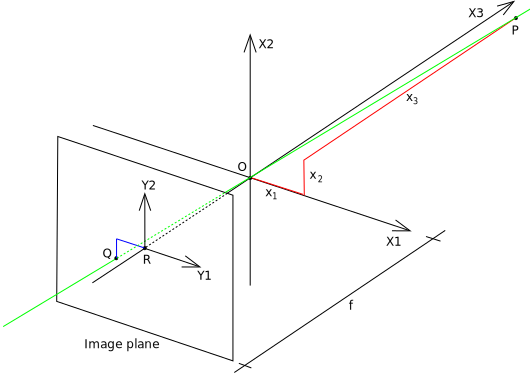
\includegraphics[width=0.7\textwidth]{pinhole3d}
}{fig:pinhole3d}{
	Pinhole camera geometry.
	Camera coordinate system origin at O, axis X3 points towards the optical axis, Y1 and Y2 point to image plane axes and R is the principal point, at the image center.
	The point P projects to Q, as well as everything else on the line joining them.
	The image plane is f units away from camera origin; f is called the focal length.
}
% FIXME z left handed?

Light rays travel through the pinhole camera's aperture to the image plane that is $f$ units behind the aperture, while the camera origin is set to the aperture.
The pinhole model (or, perspective projection) states that the world point $(x, y, z)$ is projected to the 2D image plane at $(u, v)$:

\begin{equation}
\begin{pmatrix}
u \\ v
\end{pmatrix}
=
-\frac{f}{z} \begin{pmatrix}
x \\ y
\end{pmatrix}
\end{equation}

The result can be derived from similar triangles with a common vertex at the aperture; Figure \ref{fig:pinhole3d}.

Sometimes the sign is inverted, which results in a plane on the other side of the origin where the actual point lies, where the image is not rotated; this can be more convenient to analyse.
Physically, the projected point in a camera is behind the aperture, on the sensor.
\cite{hartley03multiview}

%Setting the camera to origin, the mapping is given with a camera matrix as
%
%\begin{equation}
%\begin{pmatrix}
%u \\ v \\ 1
%\end{pmatrix}
%=
%\begin{pmatrix}
%xf/z \\ yf/z \\ 1
%\end{pmatrix}
%\sim
%\begin{pmatrix}
%x \\ y \\ z/f
%\end{pmatrix}
%\sim
%\begin{pmatrix} \label{eq:cmat}
%	1 & 0 & 0 & 0 \\
%	0 & 1 & 0 & 0 \\
%	0 & 0 & 1/f & 0
%\end{pmatrix}
%\begin{pmatrix}
%x \\ y \\ z \\ 1
%\end{pmatrix}
%\end{equation}

The camera position and rotation in a global coordinate frame are encoded in a matrix transformation, so that the point $(x,y,z)$ in global coordinate frame is first transformed from a global coordinates to a camera-centered frame.
% Matrices, homogeneous coordinates.

% projective element, "~" up to scale equality definition

In computer graphics and vision, points and directions are usually described in \emph{homogeneous coordinates}.
Homogeneous coordinates add an extra dimension to the interpretation of coordinates, and each point becomes a line that crosses the origin in a dimension one higher than the original.
In addition, several vector operations become more convenient to manipulate; for example, 3D translation is embedded in 4D matrices with homogeneous coordinates. \cite{hartley03multiview,heyden2005multiple}
%Translation, perspective projection, rotation, and other operations are conveniently described as matrix transformations by using an additional dimension for points: $(x, y, z, 1)$.
The space is scale-invariant; all points $(xw, yw, zw, w)$ map to the same 3D point $(x, y, z)$.
\cite{dubrofsky2009homography,hartley03multiview}

%Homography definition (mapping of points and lines in $P^2$)

The imaging process essentially captures a projection to a flat two-dimensional plane of the camera's view.
When comparing points between different cameras that view the same scene, the cameras' relative positions and rotations must be known.
One of the cameras is often conveniently chosen as the origin of a global coordinate frame, so that its extrinsic parameters become unity transforms (programming libraries may assume this, see e.g. \cite{opencv}).
Each three-dimensional point in the world is transformed to the small sensor inside the camera, which is then digitized to a discrete two-dimensional grid of pixels, with different coordinate units.

%Figure \ref{fig:TODO} illustrates this transformation chain, which is encoded as the following equations, given a homogeneous point (4-dimensional vector) $X$ representing a 3D location described in physical (e.g. metric) coordinates:

The transformation chain is encoded as follows in eq. \ref{eq:projxform}, given a homogeneous point (4-dimensional vector) $X$ representing a 3D location described in physical (e.g. metric) coordinates:

\begin{align} \label{eq:projxform} \begin{split}
	x
	&= M_i X_s\\
	&= M_i M_p T R X\\
	&= M T R X\\
	&= P X\\
\end{split} \end{align}

$x$ is a 2d pixel in a discrete image, $X_s$ exists on the sensor.
$R$, $T$ encode the camera rotation and translation (extrinsics);
$M_p$ projects the world coordinates to the camera sensor - still in world coordinates, and finally the affine $M_i$ transforms the points from the sensor to pixel coordinates on the digital discretized image.
The transformation pipeline is depicted in Figure \ref{fig:projxformworld}.

\simplegfx{p}{1.0\textwidth}{projxformworld}{
	Transformations in a projection matrix pipeline.
	FIXME: draft image
}


The whole projection $P = M_i M_p T R$ can be used as-is without decomposing it to separate matrices, unless the individual parameters are needed.
The matrices $M_i$ and $M_p$ are usually not decomposed but presented as a whole intrinsic matrix.
As the chain consists of several matrices, some of them are defined only up to scale; the coordinate systems' units can be chosen freely.
Software packages usually do not decompose the chain, because it is not needed and unique parameters cannot be found because of scaling.

%The external camera parameters are called the extrinsics: camera coordinate system position and rotation (heading) in the global space.
%Camera position sits at the projection center blah.

The internal parameters, intrinsics, encode how the image is formed on the sensor: they consist of focal length $f$, pixel size ($m_x$ by $m_y$) and principal point $(u_0, v_0)$:
% FIXME 3x3 3x4 4x4
\begin{equation}
	M =
	\begin{pmatrix}
		m_x & \gamma & u_0\\
		0   &    m_y & v_0\\
		0   &        0 & 1
	\end{pmatrix}
\cdot
	\begin{pmatrix}
		f & 0 & 0\\
		0 & f & 0\\
		0 & 0 & 1
	\end{pmatrix}
	=
	\begin{pmatrix}
		\alpha_x & \gamma   & u_0\\
		0        & \alpha_y & v_0\\
		0        & 0        & 1
	\end{pmatrix}
\end{equation}

For simplicity, it is often denoted $\alpha_x = m_x f$, $\alpha_y = m_y f$.
$R = (u_0, v_0)$ is the image center (or principal point).
The parameters can also be presented separately without the matrix notation.
For square pixels, $m_x = m_y$, and for a non-skewed (rectangular) sensor, $\gamma = 0$, which is often the case. \cite{hartley03multiview,szeliski10vision,heyden2005multiple}

%Le image. Horizontal planar triangle, lines between camera origins etc. lecture11.pdf.

% }}} coord systems and transforms

\subsection{Camera calibration} % {{{

\emph{Calibrating} a camera means \emph{measuring} its intrinsics and extrinsics in order to map its data to a known coordinate frame.
Reconstruction algorithms relate points between images to recover depth; the relations are specified via camera parameters.
Calibration is not necessarily a manual step before scanning;
self-calibration and structure from motion techniques can recover camera calibration from a static scene automatically. \cite{pollefeys1999hand,hartley03multiview}

It is sometimes convenient to store intrinsics and extrinsics separately if the intrinsic matrix is constant for several pictures, for example;
the intrinsics can then be calibrated beforehand only once.
For a camera rig that does not change, whole intrinsic and extrinsic calibration can be retrieved beforehand and applied on further scanned datasets for direct reconstruction.

Manual calibration is done with a known pattern, such as a planar checkerboard pattern \cite{chuang2002performance,zhang2000flexible} or manually selected point pairs.
A known pattern is fast to detect and results in correct physical units when the physical pattern size is given.
The checkerboard calibration step is often programmed to measure optical distortion at the same time. \cite{opencv,camcalmatlab}

A single image of a three-dimensional calibration object is also sufficient for single-camera calibration. \cite{jokukirjoist}

One way for calculating the calibration is direct linear transform (DLT):
the whole matrix $P$ is solved from $x_i = PX_i$ by constructing a system of equations from the projections of some known points $i$, and minimizing an error metric, as the case is usually overconditioned. \cite{hartley03multiview}

A video-based method has been proposed by Svoboda for self-calibration.
The method uses a number of synchronized frames and a laser pointer in a dark calibration volume to find corresponding points, not requiring any precise objects. \cite{svoboda2005convenient}

Structure from motion recovers full calibration for a larger amount of cameras with given matching point pairs, with no special requirements on the subject.
It can be used to calibrate an arbitrarily large unknown set of cameras automatically.
It is described further in section \ref{sec:sfm}.

%Projective calibration only is too general, as it leaves out some assumptions that can be done about a physical world, such as relative angles and sizes; metric calibration something something. \cite{zisserman1995metric}.

%Methods that dig the matrix out of a single image have certain restrictions, and won't work if e.g. seven points lie on the same plane [longuet-higgins etc.]

%many single planar chessboard pics vs. a single image of an accurate 3d model.
%Single three-dimensional calibration object is also sufficient blbl

%cv::stereocalibrate, cv::calibratecamera
%TODO Figure: show extrinsic in matlab cam calibs, nice pics (both cam and world centered)

% }}} camera calibration

\subsection{Preprocessing/normalization} % {{{

(to be moved)

%The scale of values in the equations above affects the precision [hartley, in defense of .., h,ziss]. 
The scale of values affects the numeric precision \cite{hartley1997defense,hartley03multiview}.
A similarity transform is used to modify the values to a more consistent range.
Centroid is moved to image center, and the coordinate axes are scaled.

%Translate centroid to the origin, scale so that average becomes sqrt 2.

Histogram and brightness equalization is done if image brightnesses vary for more effective point matching.
A well controlled stereo rig does not need color correction if the lighting is even enough.

% }}}

\subsection{Calibrated stereo vision} % {{{

Given two or more views of a same scene, depth for a point can be extracted by comparing the positions of the point in different views.
Whole-picture depth extraction results in a depth map imaged from a single view, giving a depth value for each pixel in a picture, resulting in a set of three-dimensional points seen by that view.
The resulting stereo vision consists of many steps.
In order to compare the point positions in two images, given a point in one image, its matching pair must be found on the other.
In the following section, this search problem in finding corresponding pixels, mapping them so that they can be compared, and the comparison that results a depth value are formalized.

% }}}

\subsubsection{Binocular disparity} \label{sec:binocular} % {{{

%Essential, fundamental matrices. Correspondence problem. Rectification, undistortion. Epipolar geometry.

\simplefig{h!}{
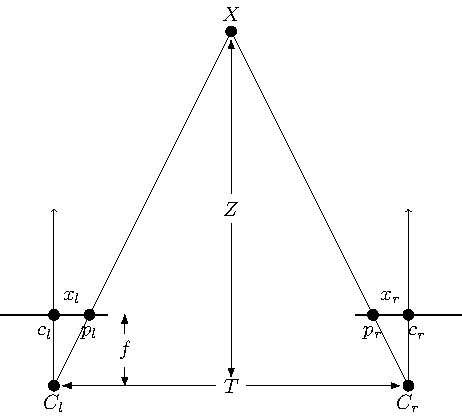
\includegraphics{simplestereo}
}{fig:simplestereo}{
	A very simple stereo setup, pictured from above.
	The image planes (thick lines) are actually imaginary, as a real film in a camera would exist behind the principal point and project the image as rotated around principal axis, as described earlier in \ref{sec:imaging}.
	The coordinates are given in units of the world coordinate system, common with the camera origins.
	The symbols $C$ are the camera origins ($T$ units between each other); $c$ the principal points; $x$ the image plane coordinates of $p$ w.r.t.~the principal points; and $f$ is the focal length.
	The unknown is $Z$, i.e.\ depth of point $X$.
}
% this figure would need to be bigger and have also the back side planes (sensors) as opposed to the (normalized?) image planes (at f=1?)

%Next, the setup of binocular stereo vision is described. Common stereo vision rigs use the simplest possible case: two identical cameras with a fixed distance, both oriented to the same direction, parallel to the line connecting them, as in Figure \ref{fig:simplestereo}.

%Assuming known calibration with identical cameras (same focal length and sensor) in a setup described above, visualized in Figure \ref{fig:simplestereo}, points can be triangulated as follows:
Assuming a planar setup with identical cameras (same focal length and sensor) facing in the same direction as visualized in Figure \ref{fig:simplestereo}, points can be triangulated as follows:

From similar triangles with a common vertex at $X$, we get (note that $x_r < 0$ as it's to the left, towards to the negative axis, from the corresponding plane's origin):

\begin{align} \label{eq:triangulation} \begin{split}
	\frac{Z}{T} &= \frac{Z-f}{T - x_l + x_r} \\
	&= \frac{Z-f}{T - d}\\
	ZT - Zd &= ZT - fT\\
	Z &= \frac{fT}{d}
\end{split} \end{align}

The disparity $d$ is the difference of the points in their image planes, $d = x_r - x_l$.
%If the image planes would be fixed as being physically correct, in the back side of the camera origins, the focal length should be negated to keep the correct interpretation and sign because the projected physical image is mirrored in both axes.
%Image processing between the sensor and a picture file usually inverts this.
As the equation \ref{eq:triangulation} shows, depth is inversely proportional to pixel disparity in the images.
To map the depth to correct units, only focal length $f$ and the baseline $T$ are needed additionally; when using pixel coordinates instead of physical in $d$, also the pixel size should be taken into account in scaling $x_l$ and $x_r$.
All of these are encoded in the camera parameters: the pixel size is part of the intrinsics, and the baseline is encoded in extrinsics.
Algorithms such as those in OpenCV \cite{opencv} can compute depth from disparity images based on the difference between each pixel.
The disparty image is a difference of each pixel value, which needs a search for each pixel;
this is discussed in the following.

% }}} binocular disparity

\subsubsection{Epipolar geometry} % {{{

\simplefig{h!}{
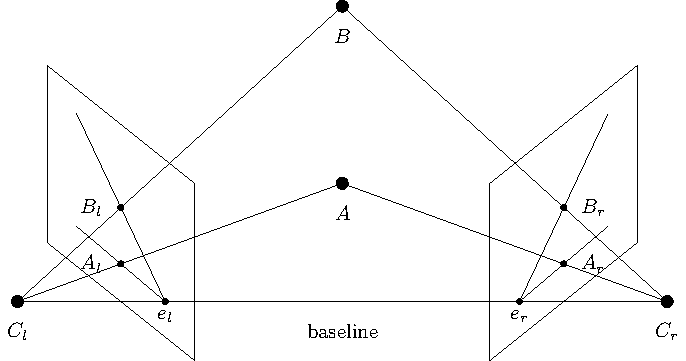
\includegraphics{epigeom}
}{fig:epigeom}
{Two camera views on same scene.
World points $A$, $B$ project to planes of different views imaged from $C_l$ and $C_r$ on the left ($A_l$ and $B_l$), and to the right ($A_r$, $B_r$).
The actual images cover some area of the total projection plane, and the epipolar point may or may not lie visible in the image.
When $A_l$ is known, its corresponding point $A_r$ (not initially known in practice) is found on the epipolar line joining $e_r$ and $A_r$ in the right image.
All epipolar lines in a view join in the same point ($e_l$ and $e_r$).}

% TODO: small algorithm for pairwise windowed point matching on the line (hox! and link to point matching section maybe)

In stereo vision, the same scene of interest is seen by two or more cameras at the same time.
The cameras are rarely aligned perfectly as in the disparity setup described above, however.
\emph{Epipolar geometry} encodes the relations between arbitrarily positioned cameras in a standard way so that coordinates of a 3D point seen in several images can be calculated with similar triangulation.

As seen in Figure \ref{fig:epigeom}, a point seen by camera $C_l$ at 3D point A could be anywhere on the line between $C_l$'s origin and A, because a certain line passing through the principal point always projects to a point.
This line is seen as a single point $A_l$.
From another viewpoint in camera $C_r$, this line equals to some line on the right image plane.
The matching point must be on that line.
The inverse applies for any point on $C_r$ and a line on $C_l$.
These special lines on the image planes are called \emph{epipolar lines}, and they all coincide at a special point called \emph{epipole}, $e_l$ and $e_r$.
For example, the line from $C_l$ to $A$ projects to the line from $e_r$ and $A_r$ on the right plane, and likewise, the line from $C_l$ to $B$ projects to the line from $e_r$ and $B_r$, which can be easily seen from the triangles in the figure.

% FIXME:
\emph{Essential matrix} encodes how the camera poses differ, to match one image's point in another.
When $A_l$, $A_r$ encode the points in Figure \ref{fig:epigeom} by the corresponding camera coordinates, and the baseline difference is a vector from $C_l$ to $C_r$, it holds that $(A_l-C_l) \cdot (C_r - C_l) \times (A_r-C_r) = 0$, as all the vectors are coplanar; the cross product yields a normal to the plane, which is perpendicular to all the vectors, thus the dot product equals 0.
\cite{hartley03multiview}
Essential matrix $E$ is a matrix form of this relation; it includes the relative rotation and translation of the two cameras:

\begin{equation} \label{eq:essential}
	A_l E A_r = 0
\end{equation}

%\begin{align*} \label{eq:essential}
%	%A_r &= R (A_l - t) \\
%	%A_r^T R T A_l &= 0 \\
%	%A_r^T E A_l &= 0
%	A_l \cdot t \times A_r = 0\\
%	A_l \cdot t \times R A_r = 0\\
%	A_l^T T
%\end{align*}

%where $T$ is the cross-product form of $t$ encoded in a matrix form as below. The essential matrix is obtained as $E = R T$.
%
%Le image. lecture11.pdf. O->p dot (O->O' cross O'->p') = 0
%
%Cross product expressed in a skew-symmetric matrix form is
%\begin{equation}
%\vec a \times \vec b =
%\begin{pmatrix}
%	 0   & -a_z &  a_y\\
%	 a_z &  0   & -a_x\\
%	-a_y &  a_x & 0
%\end{pmatrix}
%\begin{pmatrix}
%	b_x\\b_y\\b_z
%\end{pmatrix}
%= \vec c
%\end{equation}

\emph{Fundamental matrix} is a similar object; it also relates the corresponding points in stereo images.
It has the same meaning as the essential matrix, but it works in the pixel coordinates of the cameras, which are obtained after the projective transform that takes the intrinsics into account; that is, it encodes also intrinsic parameters.
%Inverting the matrix $M_i$ (section \ref{sec:coord}) in sensor-to-pixel coordinate transform and using it on pixel coordinates, world coordinates seen on the camera sensor can be obtained. % FIXME equations

Given pixel coordinates $a_l$ and $a_r$ that match the points $A_l$ and $A_r$ as seen from cameras $C_l$ and $C_r$, respectively, the fundamental matrix $F$ is given as:

\begin{equation} \label{eq:fundamental}
	a_l F a_r = 0
\end{equation}


%\[
%\hat pAl = M_p A_l\\
%\hat A_r = M_p A_r
%\]
%
%and using it on pixel coordinates, the world coords can be obtained, plugging in to the equation \ref{eq:essential}
%
%\[
%A_r^T E A_l = 0\\
%(M_p^-1 \hat A_r)^T E (M_p^-1 \hat A_l) = 0\\
%\hat A_r^T M_p^-T E M_p^-1 A_l = 0\\
%\hat A_r^T F \hat A_l = 0
%\]
%
%the fundamental matrix
%
%\[
%F = M_p^-T E M_p^-1 = M_p^-T R T M_p^-1
%\]

The fundamental matrix relates directly the pixels and epipolar lines, and as such it is useful in image processing where the images are described as pixels in a raster image rather than physical coordinates.

%Le image above and lecture11.pdf. O->p dot (O->O' cross O'->p') = 0

%Cross product expressed in a skew-symmetric matrix form is
%\begin{equation}
%\vec a \times \vec b =
%\begin{pmatrix}
%	 0   & -a_z &  a_y\\
%	 a_z &  0   & -a_x\\
%	-a_y &  a_x & 0
%\end{pmatrix}
%\begin{pmatrix}
%	b_x\\b_y\\b_z
%\end{pmatrix}
%= \vec c
%\end{equation}
%
%Epipole can be interpreted as the location of another camera as seen by other camera, as seen in the picture.

%Now, given its position in the image plane of camera $C_l$ and the fundamental matrix $F$, finding the corresponding point in camera $C_r$'s image plane is seen as solving eq. \ref{eq:fundamental} for $a_r$.

The essential and fundamental matrices can be seen as a more general configuration of the triangulation in Figure \ref{fig:simplestereo} and eq. \ref{eq:triangulation}.
Once the points are found by solving \ref{eq:fundamental}, the depth can be obtained.

% cite longuet-higgins 1981, the books too

% }}} epipolar geometry

\subsubsection{Features and point matching} % {{{

%salient geometric features for matching

Previously, basics for reconstructing a three-dimensional location for a point pair were introduced, assuming known positions for the same point in different images.
To reconstruct a whole scene from a full image, all pairwise points must be \emph{matched}, i.e.\ found that what pixel in one view represents the same object as one in other view.

Matching is often also called \emph{correspondence} searching:
Given a pixel in one image, what is the corresponding pixel in another image taken from the same scene?
Pixels correspond to each other if they represent the same physical point.
Matching pixels for the previously introduced methods are found in the image space by comparing the color neighborhood.

% FIXME: pairwise feature matching vs. windowed matching
% TODO some sift descriptor theory, angle histogram stuff

To describe the pixel's visual characteristics, its surrounding environment is encoded as a \emph{feature}, an easily recognizable property vector, \emph{feature descriptor} or \emph{feature vector}.
%When discussing about features, not every pixel's neighbourhoods are used; \emph{good} features are those that have strongly distinguishable properties, such as edges and corners.

Edges or corners are essentially high-frequency information in the image that can be interpreted as a 2D discrete function; thus, they can be detected by a discrete high-pass or band-pass filter, zeroing all but those pixels where a high difference is found. \cite{marr1980theory}
Many feature detector algorithms are based on edge detection. % CITE

Scale-invariant feature transform (SIFT) \cite{lowe1999object} is a well-known algorithm for local feature detection. A fast GPU implementation is also available \cite{changchang2007siftgpu}.  Invariance to scaling and rotation makes SIFT useful in describing features that can be matched between unaligned images. Other similar commonly used means are Speeded Up Robust Features (SURF) \cite{bay2006surf}, Harris corner detector \cite{harris1988combined}, and difference-of-gaussian-based (DoG) methods \cite{dog}.

Searching for well distinguished features in an image is called \emph{sparse} search.
A sparse set of feature matches is good for reconstructing initial calibration, as all the feature vectors can be matched together relatively quickly.
For finding a complete depth map of the whole image, a slower \emph{dense} search is performed, using the obtained calibration.
Dense matching runs through each pixel of the search space and tries to find a matching pixel from another image with e.g. template matching \cite{duda1973pattern}.
The surrounding pixel values themselves inside a \emph{window} centered at the searched pixel are compared in the search area.

From the coordinate differences in image space between the two images, a disparity map is built.
The disparities can then be directly transformed to depth values, yielding a point cloud.
Other more sophisticated algorithms too find dense matches but may not use a disparity map.

% }}}

\subsubsection{Image rectification} % {{{

% rectification pics

In order to triangulate a 3D point from two photographs, the location of the point in both the images must be known.
The dense correspondence search is not done with feature matching but comparing pixels directly instead.
Given a single pixel in one image, its corresponding pair would naively be searched by looking at every possible pixel in another.

Rectification is a process that simplifies this search problem by restricting the search to a single dimension using the epipolar lines.
Further, closeby points are only looked in a small window around the previous, not spanning the whole search space.

By virtually aligning the cameras such that their images are coplanar, the search only has to be performed on a line that is parallel to the line connecting the camera centers.
Rectification can be done in multiple ways.
Planer rectification projects the images on a common plane and rotates them such that corresponding lines are axis-aligned (horizontal or vertical) in both images. \cite{hartley03multiview}
In Figure \ref{fig:rectif}, two cameras are situated at arbitrary positions, looking at different directions, and their view images are projected on a common plane, where they show up as trapezoids.
In practice, a new image can be created that contains the old trapezoidal image, or the search can be performed in the original image in the direction of the epipolar line.

\simplegfx{h}{0.6\textwidth}{rectif}{
	In planar image rectification, two images are twisted so that the epipolar lines (drawn in red) become parallel.
}


%Rectified images are twisted so that todo todo, see Figure \ref{fig:rectification} compare to epipolar geometry image, epipolar lines become parallel in the rectified images
% LOL TODO guido gerig image rectification (stereo) slides

% }}} correspondence and rectification

\subsubsection{Multi-view stereo} % {{{

% zhang snavely curless 2004 real time dense 3d face capture spacetime stereo

(highly incomplete section)

% nelliportaali:pikahaku multiview stereo reconstruction
%graph cuts
%\cite{jancosek2011multi}
%\cite{chang2011gpu}
%(this section needs expansion and pictures)
% if no information about camera parameters is available, pairwise checks between the images may become expensive. \cite{wu2013towards}
%evaluations in \cite{goesele2007multi}
% se zephyrpapru jossa algossa per kamera depth ja merge

% intro

\emph{Multi-view stereo} (MVS) is stereo vision using more than two cameras.
In the literature, MVS refers to both the big picture of a whole reconstruction pipeline using several pictures, and just the dense reconstruction after system calibration has been done.
Reconstruction using a large set of cameras has two distinct major ways to perform:
One way is to extend the two-view geometry theory further to many cameras, recovering the whole subject at once using many views simultaneously.
Other, also commonly used method is to arrange the cameras in binocular pairs, reconstruct each pair separately to obtain a depth map from each pairwise view, and finally merge the resulting points to a single set. \cite{bradley2010high}

% epipolar in N

The case of more cameras than a single pair uses the same epipolar geometry principles, extended in several ways.
More cameras bring more dimensions, complications and also restrictions that can be utilized.
In three-view geometry, for example, the fundamental matrix becomes three-dimensional, the trifocal tensor, relating all three cameras to the others. \cite{hartley03multiview}

Some suggest to find a set of initial features and expand them to nearby pixels. \cite{furukawa2010accurate, regiongrowingtodo}

Multiple baseline stereo is a simple special case for many cameras. When all the cameras lie on the same baseline, calibration is easier and points seen by all cameras can be selected simply by using a minimized sum of errors. \cite{okutomi1993multiple}

An incremental algorithm linear-time in number of the cameras has been suggested for SfM for large-scale reconstructions. \cite{wu2013towards}
A specialized scanning rig in this work is not considered large-scale.
Large-scale refers to hundreds or even thousands of images of a huge geometry, such as an outdoor building or terrain.
A state-of-the-art patch-based reconstruction combined clustering to split large-scale datasets produces dense, oriented point sets \cite{furukawa2012patch,furukawa2010accurate}

Toldo et al. suggests to build a depth map individually per each view with approximated normals, and to combine the points to a mesh with Poisson surface reconstruction. \cite{toldo2013accurate,toldo2013towards}

% }}} multi-view stereo

\subsection{Structure from motion} \label{sec:sfm} % {{{


The \emph{structure from motion (SfM)} problem, also called structure and motion, uses the scene feature matches between different views to determine both the scene structure and the camera motion between the views.
\cite{snavely2006photo,fitzgibbon1998automatic} 
The camera does not have to physically move; the method can be used for multi-camera reconstruction with a static rig.
Before SfM, the images should have been rectified and features matched; the algorithm works on point locations instead of input images.
While SfM retrieves the scene structure and camera parameters, a dense reconstruction usually follows it as only a fraction of the points in the images need to be considered.

SfM begins with two reference views that are used to retrieve an initial reconstruction, and extends each new view into the set iteratively.
Lastly, a \emph{bundle adjustment} method is used to globally optimize the scene parameters. \cite{triggs2000bundle}
The relation between the views need not be previously calibrated; the process determines camera poses.
In fact, many reconstruction applications use structure from motion as an initial step to determine calibration and proceed then to dense reconstruction.

The initial stage builds a reference frame and structure for the selected features (points) in two cameras.
% pollefeys tutorial builds the frame using the epipolar geometry, determined as previously in section \ref{sec:epipolar}.
The structure is determined with triangulation as in section \ref{sec:binocular}.
In practice, perfect reconstruction cannot be achieved due to noise, and the points are found by minimizing a reprojection error to the extent of a specified threshold limit.

After a coordinate frame is built as a basis using two views, the next camera views are iteratively added to obtain an initial estimate of the camera poses and the selected scene feature positions.
Scene features can be matched between only last few views if the camera motion is known to be continuous;
the matches can also be done between all possible image pairs, which is feasible if there is lots of overlap.

As a last step, bundle adjustment globally optimizes the bundles of light rays from the scene to all cameras.
Several algorithms and implementations are available, while the basic idea and the underlying problem is the same:
a cost function is used to optimize jointly all camera parameter estimates such that the reprojection errors are minimized through all views.
Pollefeys \cite{tutorial} gives the following formula to minimize:

\begin{equation}
	\text{min}_{P_k, X_i} \sum_{k=1}^m \sum_{i=1}^n D(x_{ki}, P_k X_i)^2
\end{equation}

when the goal is to find the projection matrices $P_k$ and the 3D points $X_i$ for all views $k$ and points $i$, where $D(a,b)$ is the Euclidean distance and $x_i$ the known, fixed matching 2D image feature positions for each unknown 3D point $X_i$.
In practice, this nonlinear optimization problem is approached in iterative means.

According to \cite{wu2013towards}, bundle adjustment should be performed using a Levenberg-Marquardt or Preconditioned Conjugate Gradient method.

Beardsley et al. use an iterative extended kalman filter \cite{beardsley1997sequential}
% XXX others?

% }}}

\subsection{Error metrics} % {{{

The quality of the reconstruction is measured by reprojecting the 3D points back to the cameras with the estimated parameters, and calculating the distance between the projected and the matching original point, the \emph{reprojection error}. \cite{hartley03multiview}

Furthermore, if the scene structure is known beforehand (e.g.\ as a calibration object, whose physical properties are measured), the resulting quality of the structure can be compared to ground truth.
Ground truth data can also be obtained with a real 3D scanner, such as a laser ranging device. % david

%Noise in subpixel-accurate match detection and (TODO survey errors, that one .doc) affects each reconstructed depth.
In addition, uncertainty in depth depends more heavily on the pixel errors (i.e.\ disparity) if the baseline is short, depicted in Figure \ref{fig:disparityerror}. % TODO image, recent in the paper notebook

Bundle adjustment optimizes uncertainty in camera poses and projection matrices together.

When sparse feature matches are searched for matching picture points in different views, a number of features are first generated for each picture, and the matches are tested against picture pairs.
False positive matches should be filtered out; common way to handle feature errors is Random Sample Consensus (RANSAC).
Random subsets of the sample space is iterated, and samples that do not fit well to a model that is constructed for a smaller set are ignored.
The iteration that matches most samples is selected. \cite{hartley03multiview}

%Detail calculation (error on surface ~= avg reprojection error?) compute millimetres

Practically, the camera sensor size and focal length in physical units (millimetres) are known, making conversion from pixel units to millimetres possible.
Units originating from reconstruction of raster images can be simply scaled to millimetre units, resulting in more intuitive error interpretation.

%Compare to algebraic, geometric etc.

%Mesoscopic level shape reconstruction

% }}}

\subsection{Surface fitting} % {{{

A multi-view reconstruction results in a set of three-dimensional points, with no \emph{connectivity information}, i.e.\ interpretation of \emph{surfaces}.
In reality, all the pixels are projections of nearby surfaces, and a more natural and standard representation can be obtained by fitting a surface on the points.
Surfaces in computer graphics are described as collections of small patches with a polygon outline, often just triangles.
When rendering the points on a computer screen, pixels between them are interpolated to contain all color information available in the source photographs.

% }}} surface fitting

\subsubsection{Data structures} % {{{

\simplefig{h}{%
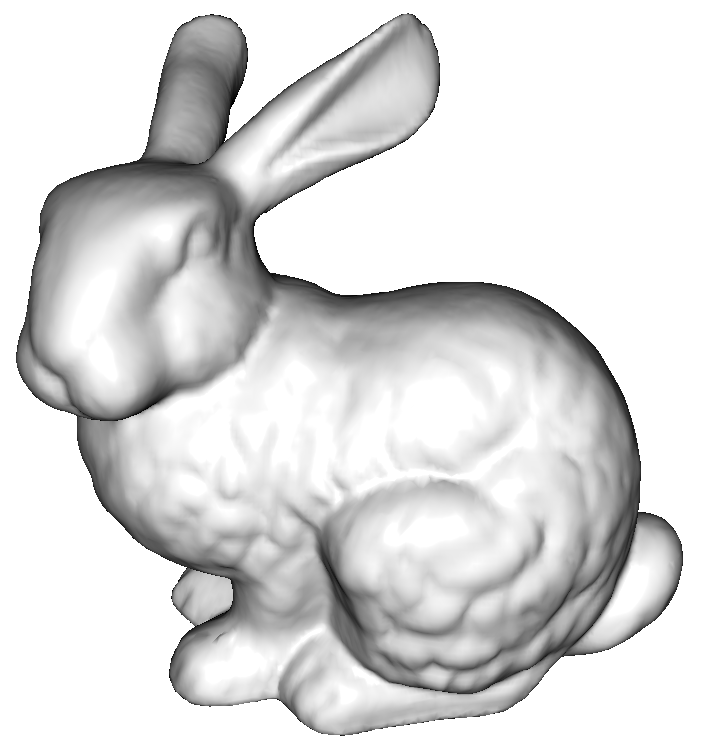
\includegraphics[width=0.3\textwidth]{bunny}
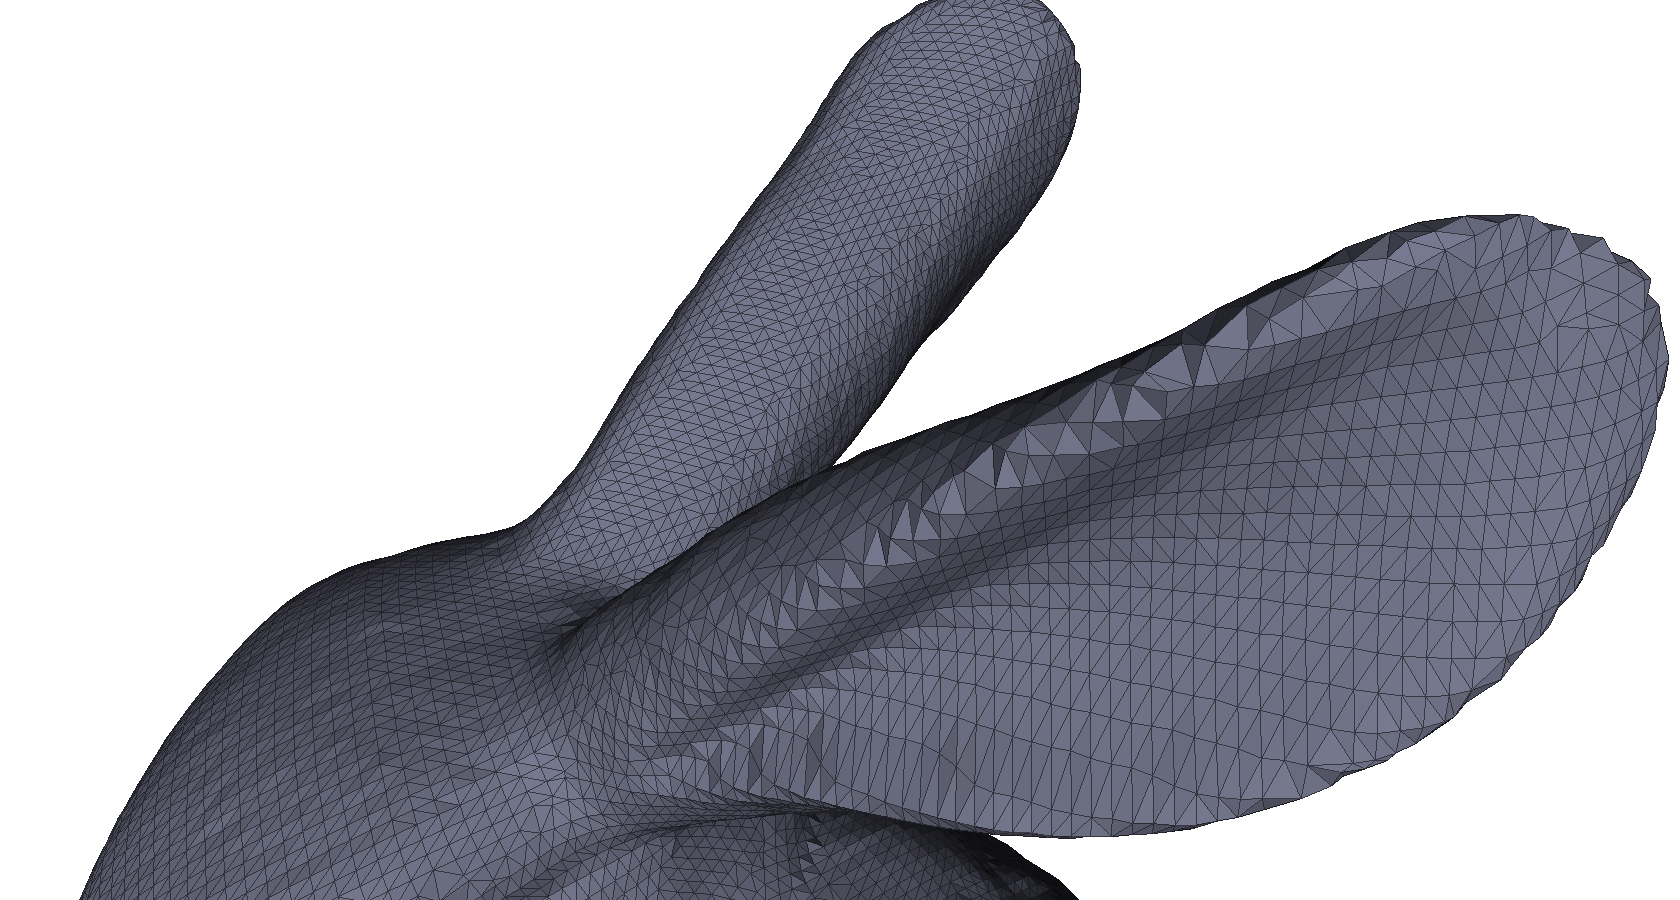
\includegraphics[width=0.6\textwidth]{bunnyear}
}{fig:stanfordbunny}{
	Stanford Bunny, a standard 3D test model by The Stanford 3D Scanning Repository, Stanford Computer Graphics Laboratory, scanned with a laser ranger.
	On the left: the whole model, shaded with a simple Phong model.
	On the right: a closeup of the left ear, showing the borders of the faces as black lines connecting the vertices.
}

% http://en.wikipedia.org/wiki/File:Mesh_overview.svg

(Should some of the main terms be defined in the beginning of the whole thesis? Probably...)

A \emph{(polygon) mesh}, a data structure often used to describe 3D models, consists generally of \emph{vertices} connected by \emph{edges}, forming \emph{faces} of objects.
The meshes often consist of triangles, which is the simplest possible polygon.
Polygon meshes have a \emph{topology}; the connectivity information of vertices on a surface, describing neighbours of each point.
Surface \emph{normals} describe the orientation of the polygon patches.
Figure \ref{fig:stanfordbunny} depicts the vertex structure of a 3D model.

A \emph{point cloud} is a loose term to describe a disorganized set of 3D points with no topology information; that is, a cloud consists only of a list of vertices, with possibly some attributes such as color or normal.
Point cloud is a natural output format for 3D reconstruction, as each point in the cloud maps to some pixel in a source image.
The images and the depth information of the 3D points are not enough for surface information, which is covered next.

% }}} data structures

\subsubsection{Geometry} % {{{

Assuming that the recovered 3D point cloud represents the surface of an object, the next step of interest is to recover the surface topology from the point cloud.
The point cloud is all geometric information that is available, but the images probably consist of more pixels than the number of points in the point cloud.
To work with the generated model and to render it properly with colors, it is imporant to recover the topology information.

A popular method for surface reconstruction from a point set is \emph{marching cubes}. \cite{lorensen1987marching}
The algorithm builds triangles in a divide-and-conquer approach based on whether points are inside or outside a cube in a grid.
A number of improvements have been proposed that utilize marching cubes as a final step.
The method of choice is currently \emph{poisson surface reconstruction}. \cite{kazhdan2006poisson,kazhdan2013screened}

Before fitting a surface on the points, the point data set should be processed either manually or automatically to remove outliers.
The surrounding scene might contain geometry that is not part of the scanned object, which will affect badly the surface fitting algorithm.
Specular highlights and other artifacts on the surface may also introduce outliers.
Manual work is a simple way to delete the points that are not part of the actual object, but also automatic methods exist if manually filtering the subject would be repetitive, e.g.\ many expressions on a human face.

% assuming X on the geometry to fit a model

% }}} geometry

\subsubsection{Texture reprojection} % {{{

When a polygon mesh is available, it should be rendered in color, including the areas between the original points.
The de facto method in computer graphics is to uses \emph{texture mapping} to color pixels in between the vertices, when the number of vertices is less than the number of pixels on the screen.
A \emph{texture coordinate} is set for each vertex in the mesh to \emph{map} a smaller image from the texture on to the particular polygon. \cite{heckbert1986survey}

Building the texture is done in a similar way of rendering the image on a screen or capturing a scene with a camera:
The reconstructed mesh surface is projected on the raster images, registering the image coordinates on each vertex. \cite[p. 610]{szeliski10vision} \cite[p. 98]{heyden2005multiple}
When the mesh is viewed from another viewpoint, the pre-projected texture data is used again.
Great accuracy can be acheived if a MVS structure is combined with a laser scan, by registering the point clouds generated by both together, using the laser scan as geometry and registered camera poses to project textures. \cite{liu2006multiview}
% (XXX read meshlab src, references?)
% parameterization + texturing from registered rasters

When several cameras see the same view, the correct texture must be chosen on each vertex.
The selection can be taken based on e.g. the image with highest detail or best brightness.

%use the registered raster projections to find out best textures and build uv coordinates
% TODO
\simplegfx{h}{0.6\textwidth}{texreproj}{
	Texture mapping a triangle from a color image on a virtual image plane on a computer screen as $m_v$.
	The triangle geometry is mapped on the color images, or textures, of the real cameras as $m_i$, and the triangular patch between the image vertices is stretched on the rendered triangle.
	Image from \cite[p. 98]{heyden2005multiple}.
}


% }}} textures

%\subsection{Postprocessing} % {{{
%
%(how the stored geometry is different from the rendered one; mathematical models in fragment shaders to use the texture variations / normal maps etc.)
%
%Error removal; strip outliers that do not have nearby pairs; small disconnected islands.
%
%Postprocessing: remodel the mesh (face), see what it would look like.
%Refine parameters to get a similar output as in the photos (normal map etc.), backproject.
%Use colors and highpass them; assume uniform lighting and locally uniform texture color (bradley).
%(Simply a rendering technique, that level of detail in 3D structure might not be needed).
%%Still, structured light and/or shading assumptions [shape from single image cues/shading trucco+verri p.225] done too.
%
%(video: 3d topology different in each frame; most algos do just stills. simple to combine them to a pre-recorded mesh)
%
%Rendered facial animation: on bones and stuff.
%% }}}

\clearpage
\section{Motion capture} \label{sec:motioncapture} % {{{

\emph{Motion capture} (mocap, or mo-cap) is the practice of recording object movement over time.
A recorded subject can be e.g.\ a human that has a skeletal model, possibly encoding also some skin movement.
In computer animation, the movement data is encoded as positions of certain vertices at each recorded point in time, and often post-processed to be parameterized to e.g.\ joint angles.
\emph{Surface capture} is a related term referring to a similar motion recording but happening on a locally deforming surface instead of a globally moving skeleton.

% It is possible to assume locally smooth movements in most areas; thus, a more intelligent approach should be used than simply reconstructing a new mesh for each frame and using registration to just align them.
% By making certain assumptions on high-resolution texture, very detailed bump maps can be extracted, for example, by backprojecting the expected 3d mesh to textures and refining. [CITE]

% }}} mocap

\subsection{4D data capture} % {{{

The reconstruction field uses the term \emph{4D} in the context of time-varying 3D data.
Analogous to the case of traditional 2D video consisting of separate discrete frames of pixels, a sequence of dynamic 3D data is, in a simple case, individual ``frames'' of point clouds.

For a source data in the form of video files per camera, effectively a sequence of synchronized pictures, each set of frames can be considered a static geometry on which the reconstruction would be done.
A naive alignment to e.g. previous or first frame is possible to average out the object movement if only its local surface movement is of interest.
Still, reconstructing each frame group separately would not produce the same topology for the mesh, as each frame contains a different point cloud and is not connected to the previous reconstruction, unless some algorithm that takes this into account is used.

Possibilities to correct the lack of coherent geometric structure exist.
Common ways include fitting each frame of the mesh to another pre-recorded or pre-modeled mesh \cite{somewhere,remedysoftware?} and matching to the previous frame iteratively.
%Later usage may need only the tracked positions of specific locations on the surface to deform a mesh with bone guides.

% }}}

\subsection{Geometry tracking} % {{{

%Kalman
%Fiducials / AR
%perf of cloth anim capture

The dynamic reconstruction requires tracking of individual points or objects in order to usefully handle the moved subject.
Non-static human motion capture in video gaming or movies, where post-processing time is available, rely on manual work to perfect the quality.
In realtime applications, the full frame is typically not reconstructed again, but only selected keypoints that are tracked in 2D are triangulated, and a previously scanned model is deformed based on them.
%A realtime case would need to e.g.~automatically register each frame between the previous one to use the geometry's dynamic properties.

However, the simplest tracking method is to leave tracking out completely: depending on the application, tracking might not be needed if the work done on the three-dimensional data does not need e.g. topological coherence in the time domain, but recomputes its work on each new point cloud.

%Registration and tracking of point clouds or meshes is a large topic on its own; this section reviewes only some of the most common methods presented in the literature.
%Some work with the reconstructed 3D structure; others use the source images and do additional work.

In three dimensions, a template model is often scanned beforehand that is then morphed to match the target object to keep the topology (i.e.~vertex neighborhood connectivity) constant.
This technique adapts well to non-rigid deforming subjects. \cite{bojsen2012tracking,li2009robust}
Common method also for the entertainment industry is \emph{animation retargeting}: using a completely separate character, and deforming it on each frame based on the current state of the scanned object, fitting the model's vertices to the scanned set.
% siggraph14 doghead

% }}} geometry tracking

\subsection{2D surface tracking} % {{{

%* SIFT/SURF/Harris feature tracking, reproject
%* edgels (edge pixels)

In two dimensions, the dense reconstruction step can be skipped when using only features in image space, providing real-time performance. \cite{pilet2005real}
Assuming that a precise object stays in the imaged volume, features can be detected and mapped to a point on the 3D surface, and tracked locally with no full-image reconstruction, while the tracked object is assumed to keep the same topology as a previously scanned model.

%http://en.wikipedia.org/wiki/Facial_motion_capture the polar express, beowulf
%Facial animation does not necessarily even need multi-view stereo for tracking and driving a predesigned character \cite{chuang2002performance,deng2007computer}.

Classic motion capture uses special reflective markers that are tracked in 2D with infrared cameras.
Distinctive bright markers are easily thresholded from the background, tracked, and triangulated in real time.
Markerless surface capture detects image features that are then used as virtual markers, working in a similar way.
Matching textured objects is more computationally intensive, and needs high resolution cameras.

Markerless capture is important in scanning facial movement, because time-varying texture is significant in highly dynamic and detailed deformations, such as wrinkles from different facial expressions.
Practically, scanning a neutral and wrinkled static subject beforehand and morphing between their texture is easier.

Tracking is done by looking for the same feature as in a previous frame in the neighborhood where it was previously.
State-of-the-art 2D tracking methods include Kanade-Lucas-Tomasi (KLT) \cite{KLT}, Tracking-Learning-Detection (TLD) \cite{TLD}, and Consensus-based Matching and Tracking (CMT), all based on \emph{optical flow}.
\cite{horn1981determining,gibson1950perception,beauchemin1995computation}
Given source and destination images, optical flow is the apparent motion in the scene, given as a motion vector for each pixel.
Estimating the flow is based on the brightness constancy constraint: the intensity (i.e.\ color) of the source and destination pixels is the same.
Optical flow is also used in morphing frames between frames in a video to virtually synchronize the cameras to a common clock. \cite{thatbradleyone}
% The Matrix.

%By combining the movement tracking to a mesh whose dynamics are modeled physically, motion can be estimated from a single image. \cite{decarlo1996integration} % (not in the scope)

% }}} 2d tracking

\subsection{3D registration} % {{{

Aligning two meshes or point clouds together is called \emph{registration}.
Registration finds a rigid transformation from one object to another.
For a moving subject, the method can be used to find the object movement between the frames.
Registration is also used for combining different, overlapping parts of a subject generated from different viewpoints to one larger model.

The basic idea in registration is to fit two surfaces or point clouds together so that the shapes that they present become as close as possible to each other.
The practical method of choice is iterative closest point fitting (ICP).
ICP iteratively finds a rigid transformation that minimizes the distance between every point in one mesh and its closest match in the other.
When tracking the deformation of a surface, the point sets describe a different geometry and there will always be some error.

When ICP is used locally, it can be applied to non-rigid cases too. \cite{brown2007global}

%Also e.g. ransac for removing noise. \cite{zhao2005alignment}

% kalman?

% }}} registration

%Tutkimusaineisto ja -menetelmät
% vai: multi-view stereo rig implementation
\section{3D scanning rig implementation} \label{sec:implementation}

Now that the background has been introduced, the practical part of this thesis follows.
Specifications for a 3D scanning rig are given, and different off-the-shelf camera types are compared more in depth.
Suitable cameras for the task are then selected and described, with the decisions on mechanical construction.
Control software for the rig is developed, and a survey is given on the readily available offering of reconstruction software.
Tests of the built system are given in Section \ref{sec:experiments}.

\subsection{Functional specification} % {{{

Constraints on the rig were specified in loose terms, leaving much work on the background study.
Desirable properties of the system were given as:

\begin{itemize}
	\item Ease of use and practicality: the user should not need to know the implementation details (hardware internals or algorithms) or to have programming skills to calibrate the system and acquire a 3D scan; scanning should be as simple as pressing a button
	\item Flexibility: for research purposes, many subjects should be possible to scan
	\item Mobility: the system should not rely on affixing fixtures on the walls or the ceiling, for example
	\item Detail: high resolution should be used for achieving data for state-of-the-art algorithms
	\item 3D and 4D: both static surface reconstruction and variations in geometry over time should be possible to scan
	\item Open design: by documenting the rig well and selecting readily available generic components, a similar system could be built if there was such a need, and the already built system could be easily extended
	\item Reasonable price: the total budget of all hardware and software combined should not exceed 10~000 EUR.
\end{itemize}

A general-purpose reconstruction rig has many practical matters to consider; some decisions can be judged by the understanding based on the pure mathematical background, while others are purely based on practical reasons.
Flexibility for arbitrary subjects means, among other interests, that the rig should be adjustable enough by means of camera positions and viewing directions.
Distance to the photographed target should not be too short in order to not annoy human subjects, but a too large setup may be difficult to build and needs a lot of space on the floor.
When capturing video, the frames should be synchronized among cameras as described in Section \ref{sec:video}, which might not be perfectly possible with consumer hardware.
A mobile rig should be light enough to carry, set up, and reconfigure for new subjects, but it should be rigid enough to give proper quality pictures and hold its calibrated configuration.
Cameras are chosen among pocket cameras, system cameras, and industrial machine vision systems currently in the market.

% }}}

\subsection{Camera comparison} \label{sec:cameracomparison} % {{{

Section \ref{sec:cameratypes} presented the typical properties of different camera categories in general, and compared them to technical requirements.
In this section, the focus is more on the feasibility of the properties on reconstruction, and on selecting a collection of feasible cameras fitting in the budget.

\paragraph{General problem statement}
Small subjects in the range of a metre or less introduce concerns in shallow depth of field, forcing the lens aperture small, and consequently, requiring bright lights or slow shutter speeds.
More sensitive sensor would require less light, but depth of field decreases as the sensor size increases.
As the capture environment will be a clean indoor space and the cameras will mostly be controlled remotely, features usually important to photographers such as weatherproofing or user interface are not considered.
Reliability on configurability and controllability is considered important.
Cheaper cameras fit more into a budget, offering more coverage of the subject, but they might not be properly controllable.
External shutter release mechanisms have been researched more on DSLRs than compact cameras, and most compacts do not have one;
the manufacturers do not provide official specifications of the release connector pinouts, but they have been reverse-engineered for many models by individual tinkerers.
Machine vision (MV) cameras, in contrast, support only external shutters.
Zoom-only lenses, lack of raw image output, remote configuration and manual modes, and slower processing speed leave cheaper compact cameras out of the comparison practically altogether.
More expensive models do have comparable features, and their prices rise into the same range as with DSLRs that are more understood.

\paragraph{Previous work}
Canon DSLRs have been used previously on commercial static capture setups \cite{ir-ltd,ten24,capturelab,agisoftforum,winder2008technical}.
Several hobbyists in the Agisoft forum suggest a Canon or Nikon DSLR. \cite{agisoftforum}
Commercial video capture setups may use specialized machine vision devices and hardware-accompanying or customized software for image capture and reconstruction. \cite{al2013new}
Also standard commercial video cameras have been used \cite{bradley2010high}, but their resolution is limited compared to still cameras.
Borshukov et al. used professional Sony/Panavision HDW-F900 video cameras for the movie ``The Matrix Reloaded'' \cite{borshukov05universal} producing uncompressed video, with a list price exceeding \$80,000. \cite{sonyhdwf900r}
Machine vision cameras have also been used where synchronization was especially important \cite{carceroni2002multi,bickel2007multi}; such cameras have also limited resolution.

\paragraph{Specialized hardware requirements}
Whereas self-contained consumer devices are not designed for and do not support any additional devices for capturing the imagery, machine vision devices need several high performance computers for reliable multi-camera capture because of the lack of local storage.
While each camera outputs easily 1 Gbit/s worth of raw data or more (Equation \ref{eq:gigabit-transfer}), a common desktop computer and one additional hard disk per camera is needed if the capture is long enough and does not fit in a computer's RAM, increasing the system cost and complexity.
%For a small number of cameras, existing buses on a PC might be enough, but a larger number requires even more bandwidth.
Best mechanical hard disks currently have sequential write speed up to 1-1,4 Gbit/s as measured by Tom's Hardware \cite{tomshw-hddwrite};
newer solid-state drives (SSD) generally are two to four times faster. \cite{tomshw-ssdwrite}
For covering all the bandwidth, expansion cards would be needed per camera, count depending on the camera protocol.
Most PC motherboards can accommodate only a few cards, requiring several PCs.

Transfer speeds given by specifications and theoretical maximum frame rates for typical 12-bit raw full-HD frames are listed in Table \ref{tab:busspeeds} ordered by speed; achievable rates would be less depending on bus protocol overhead.
\cite{hornberg2007handbook,ni2013choosing}
Benchmarked \cite{tomshw-sdwrite,tomshw-cfwrite} write speeds for Compact Flash (CF) and Secure Digital (SD) cards used in consumer cameras are given for comparison.
The cameras may still not support the maximum rate that can be achieved by the card, and actual speed may be less.

\begin{table}[h]
	\centering
	\begin{tabular}{l l l}
		Bus type & Max. theoretical speed & full-HD FPS\\
		\hline \\
		Camera Link & 5.44 Gb/s & 218 Hz\\
		USB 3.0 & 3.2 Gb/s & 128 Hz\\
		CF card \cite{tomshw-cfwrite} & 1030 Mb/s & 41 Hz\\
		GigE & 1.0 Gb/s & 40 Hz\\
		IEEE 1394 & 800 Mb/s & 32 Hz\\
		SD card \cite{tomshw-sdwrite} & 490 Mb/s & 19 Hz\\
		USB 2.0 & 480 Mb/s & 19 Hz\\
	\end{tabular}
	\caption{Bus speeds and corresponding naive maximum frame rates per second for 1920 x 1080 pixels x 12 bits; actual speeds would be lower}
	\label{tab:busspeeds}
\end{table}

\paragraph{Preferred properties}
A camera is required to have several properties, and the system as a whole must be taken as a global optimization problem, since some properties conflict each other.
In detail, the technical camera features that should be considered are described in Section \ref{sec:image-acquisition} and features that vary among different cameras are listed below.

On image quality:

\begin{itemize}
	\item CMOS/CCD sensor. CMOS suffers from rolling shutter in video mode, while global-shutter CCD is more expensive and rare in larger formats.

	\item Resolution and sensor size. Higher resolution covers more detail, until the optical limits of the system are reached. A larger sensor has larger pixels, and is thus more sensitive to light and results in lower noise and lower required exposure time. On the other hand, at an equivalent subject distance, a deeper DOF is achieved with a smaller sensor.

	\item Low noise. Sensor noise degrades image quality in general, adds error to subpixel position estimation and complicates correspondence search, etc.

	\item Dynamic range, i.e. bit depth of the processing pipeline. Whereas JPEG pictures have only 8 bits per color channel, DSLRs and industrial cameras use more, often 12 or 14 bits per pixel in raw format, that contains the color filter array effects before interpolation. Postprocessing without reconstruction can use the added color resolution.

	\item Lens quality. High sensor resolution is only useful if the lens is sharp enough, and color aberrations degrade image quality in general. Fixed focal length lenses have less moving parts and hold their calibration better. The performance of good lenses is usually given as an MTF, or modulation transfer function, describing the best possible contrast.
\end{itemize}

On practical matters affecting image quality:

\begin{itemize}
	\item Optical stabilization works by moving a glass element inside the lens or the sensor itself, effectively moving the image on the sensor, having also an effect on calibration.

	\item Dust reduction, if enabled for some consumer cameras, is typically implemented as high-frequency vibration of the sensor on camera startup. Moving the sensor might result in small calibration problems.

	\item Shutter lag. Lag measured between ordering the camera to take the picture to the actual moment where exposure starts should be consistent, and preferably small.

	\item Video frame rate, resolution, and compression. Cameras that support a raw format only use raw for still pictures and compress the video, as raw video is unnecessary in the consumer market and uses lots of space. For image processing, each frame should be as little compressed as possible. Some DSLRs support writing only full keyframes instead of predicted frames, resulting in higher quality and file size.

\end{itemize}

On practical matters affecting usability:

\begin{itemize}
	\item Lens features. While photography lenses typically support automatic focusing, MV lenses only have manually adjustable or fixed-distance focus. Of photography devices, compact cameras feature a non-changeable zoom lens, while system cameras feature interchangeable lenses.

	\item Continuous shooting rate, or the speed at which full-size pictures can be taken. Controlled by many factors, on consumer cameras, image processing speed and memory card write speed have most effect, and on MV cameras, the bus speed typically limits the rate and sensor speed is selected based on it.

	\item Configurability. Aperture, shutter speed and others should be manually controllable remotely, and repeatable without automatic features.

	\item Remote trigger. Practically all DSLRs have wired or wireless remote shutter releases; some machine vision cameras have optionally an external logic-level trigger input in addition to one that is set by the protocol in the data bus. Some protocols may have global commands to send throughout a group of cameras. (FireWire?) Otherwise, software trigger suffers from sporadic jitter from operating system and protocol non-determinism.

	\item For consumer cameras, USB read speed supported by the camera. Retrieving saved image or video data takes less time for faster interfaces.

	\item External flashes. Practically all system cameras can be wired to an external flash unit; only some compact cameras support this. Industrial cameras are always externally triggered, some supporting a separate independent signal and some via the transfer bus.

	\item External power supply. Not needing to charge batteries adds value to the ease of use.

	\item Weight and size. A smaller and lighter camera requires less bulky support structures.

	\item Price. With a fixed budget, cheaper cameras can cover a larger area of the subject at a time because more cameras fit in the budget.

	\item Availability. For an easily replicable system, it should be simple to purchase the hardware.
\end{itemize}

In general, good technical properties are deep depth of field, light sensitivity, high resolution, and short distance to the subject.
Practical features also count, such as availability of external power supply instead of batteries.

All the properties should be looked as a whole; especially large pixel count does not necessarily imply better pictures if the optics is not good enough.

Prices for compact cameras that have the required features go up to the same price range as DSLRs or even higher, i.e. 500 EUR and up.

Having a much smaller production rate than larger manufacturers that target consumers (such as Canon, Nikon, Pentax or Sony), MV cameras have a broad price range from a few hundred euros to thousands, well correlated with pixel count and frame rate.
Lens prices for the C-mount optics used by MV are moderate, at around 200-300 EUR.
Properties of MV hardware is typically better specified than that of consumer devices, but prices of complete systems are an order of magnitude higher.

%The price of professional video cameras leaves them out of the comparison, them being an order of magnitude more costly than average consumer devices.

% }}}

\subsection{Selected cameras} % {{{

A number of compacts, system cameras, and machine vision cameras were reviewed.
In this section, the selected key parts are described in detail.
Precise information on all hardware used can be found in Appendix \ref{app:hardwareused}.

In general, machine vision cameras were considered overly expensive, although they perform best in synchronized video and output the frames in lossless raw format.
Compact cameras do not have significant advantages over DSLRs, when comparing models where both have comparable required features, such as remote controllability and external shutter release options.
{ \color{red} FIXME: actual table of the sample models reviewed somewhere here. }
A DSLR is a good choice for still photos because of moderate price compared to image quality, and availability of usable software and best range of accessories.
Video recording is notably worse than with machine vision that can produce higher resolution, raw data, and synchronized output;
because of a price difference of almost an order of magnitude for cameras having a comparable resolution, it was decided to leave high-performance video tracking as a minor feature, and concentrate on static subjects.
Canon was chosen over others because of firmware customizability \cite{magiclantern}, previously acquired personal knowledge of the manufacturer, well specified remote control abilities \cite{canonedsdk}, and previously proven work using the same maker \cite{ir-ltd,ten24,capturelab,agisoftforum}.

\subsubsection{Canon EOS 700D DSLR}

\simplefig{h}{%
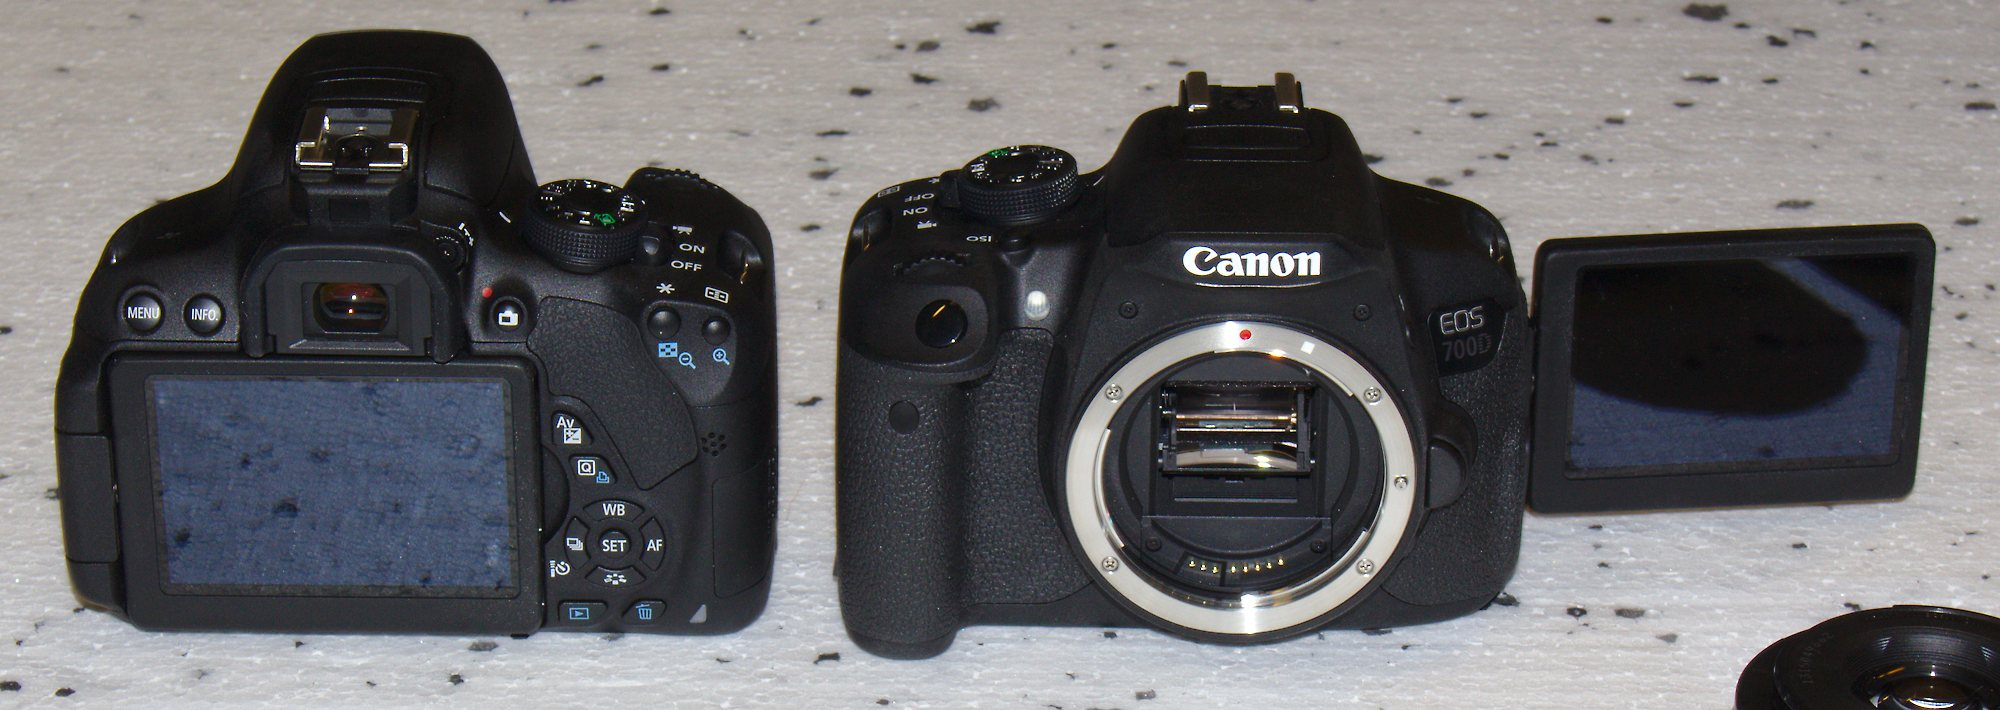
\includegraphics[width=\textwidth]{eos700d}
}{fig:eos700d}
{Canon EOS 700D DSLR camera body}

Canon EOS 700D body, also known as the Rebel T5i, introduced in 2013, is the newest of Canon's consumer range DSLRs, with a price at about 600 EUR at the point of writing.
Key features are shown in Table \ref{tab:eos700dfeatures}.
It was decided to build the rig around nine of them.
The front and back view of the camera are depicted in Figure \ref{fig:eos700d}.

\begin{table}[h]
	\centering
	\begin{tabular}{l l}
		Sensor type & CMOS\\
		Sensor size & APS-C 22.3 x 14.9 mm\\
		Pixel size & 4,3 x 4,3 $\text{\si\micro m}$\\
		%CoC span at 0.019 mm & 4.4 pixels\\ % (FIXME move to lens)
		Image resolution & 5184 x 3456 pixels (17,9 million) \\
		Processor & Canon Digital Imaging Core (DIGIC) 5\\
		Bits per pixel & 14\\
		Burst shooting speed & 5 FPS\\
		Video mode & 1080p in 30 FPS or 720p in 60 FPS\\
		Max write speed & $\approx$ 40 MB/s
	\end{tabular}
	\caption{Canon EOS 700D key features}
	\label{tab:eos700dfeatures}
\end{table}

\paragraph{Properties}
Relatively large pixel count combined to a good lens captures high-resolution detail.
The sensor's pixel size is not unnecessarily small but not as large as in full frame DSLR cameras.
%Dynamic range with 14 bits per pixel is relatively large; most reconstruction programs use 8-bit images, though.
% raw images useful for manual image enhancement
The 5 FPS continuous speed for full-size images can be used for testing high resolution motion, but the video abilities are also reasonable.
Ghosh et al. use DSLRs operating in burst mode for special illumination capture, which presents one augmentation for the rig in future work. \cite{ghosh2011multiview}
The quality can be tweaked with firmware modifications and raw video recording is also possible, at reduced resolution limited by storage speed. \cite{magiclantern}
The sensor is labeled ``Hybrid CMOS'', a new Canon's technology that embeds phase-detection autofocus pixels in the sensor for fast continuous autofocusing in video mode.
A number of pixels is missing color sparsely around the middle of the sensor and are interpolated; they only introduce artifacts in raw video.

The recent Canon EOS M MILC shares many features and internal elements with EOS 700D and was strongly considered, but it is missing support for remote shooting from USB or wired remote release.

%Older models of the same product line can still be found in the market, such as 650D or 600D.
%700D has a newer processor and thus faster processing speed, faster memory card controller and others.
Resolution of the sensor has stayed same since the EOS 550D, introduced in 2010.
At the same time, also cheaper new models are available, such as the EOS 1200D; at a reduced price, less processing power is provided, resulting in slower operation but otherwise the cameras share mostly same features.
The more expensive professional cameras vary mostly by processing speed and build quality.

\paragraph{Storage}
The camera uses Secure Digital (SD) memory cards for mass storage, supporting the UHS-I standard (Ultra High Speed).
Maximum write speed has been found experimentally to be approximately 40 MB/s \cite{magiclanternforum}.
A class 10 UHS-I memory card was selected; manufacturer claims 45 MB/s write speed.

\paragraph{Conveniences}
The camera also features a tilting LCD screen that has provided to be useful when looking the camera from the front.
Additionally, AC power adapters were chosen to operate the cameras without the need for charging batteries.
Canon sells adapters that plug in the camera's battery holder, providing continuous power at the expense of an additional cable per camera.
For wireless remote shutter, the camera natively supports an infrared remote controller that must be pointed towards the camera from the front.

% flashguns

\subsubsection{Canon EF 50mm f/1.8 II}

Canon's EF-mount 50mm f/1.8 II lens (priced at about 110 EUR), shown in Figure \ref{fig:canonef50mmlens} is well known for its excellent image quality at a low price.
The lens was introduced in 1990.
The 50 mm focal length with the crop factor of 1.6 of the camera body provides a good shooting distance for the purposes of this work.
Like most lenses at this focal length, the lens is nearly distortion free.
Despite the poor plastic build quality, its glass is of very high quality and it is well known as one of the best portrait lenses for photography.
The lens changes between autofocus and manual focus modes with a mechanical switch, and the focus ring in manual focus mode is loose enough that it might need to be locked with tape if left on for a long time shooting to hold its position for a calibrated setup.

At a distance of one metre $d = 1$ m, the sensor size of $s_x \times s_y$ = $22.3 \times 14.9$ mm and $f = 50$ mm focal length, the area that fits in the frame is $a_x \times a_y$:

\begin{align} \label{equ:areasize} \begin{split}
	a_x &= s_x \times \frac{d}{f} = 22.3 \text{mm} \times \frac{1 \text{m}}{50 \text{mm}} = 446 \text{mm}\\
	a_y &= s_y \times \frac{d}{f} = 14.9 \text{mm} \times \frac{1 \text{m}}{50 \text{mm}} = 298 \text{mm}
\end{split} \end{align}

which is easily seen from similar triangles with a common corner.
From Equation \ref{eq:dof}, the depth of field at this setting is about 16 cm for a f-number of f/11, or 20 cm for f/14, at circle of confusion of 0.019 mm (using the d/1500 rule), a reasonable depth for the given area size.
This circle of confusion would give span $0.019 mm / 22.3 mm * 5184 px \approx 4.4$ pixels.

\simplefig{h}{%
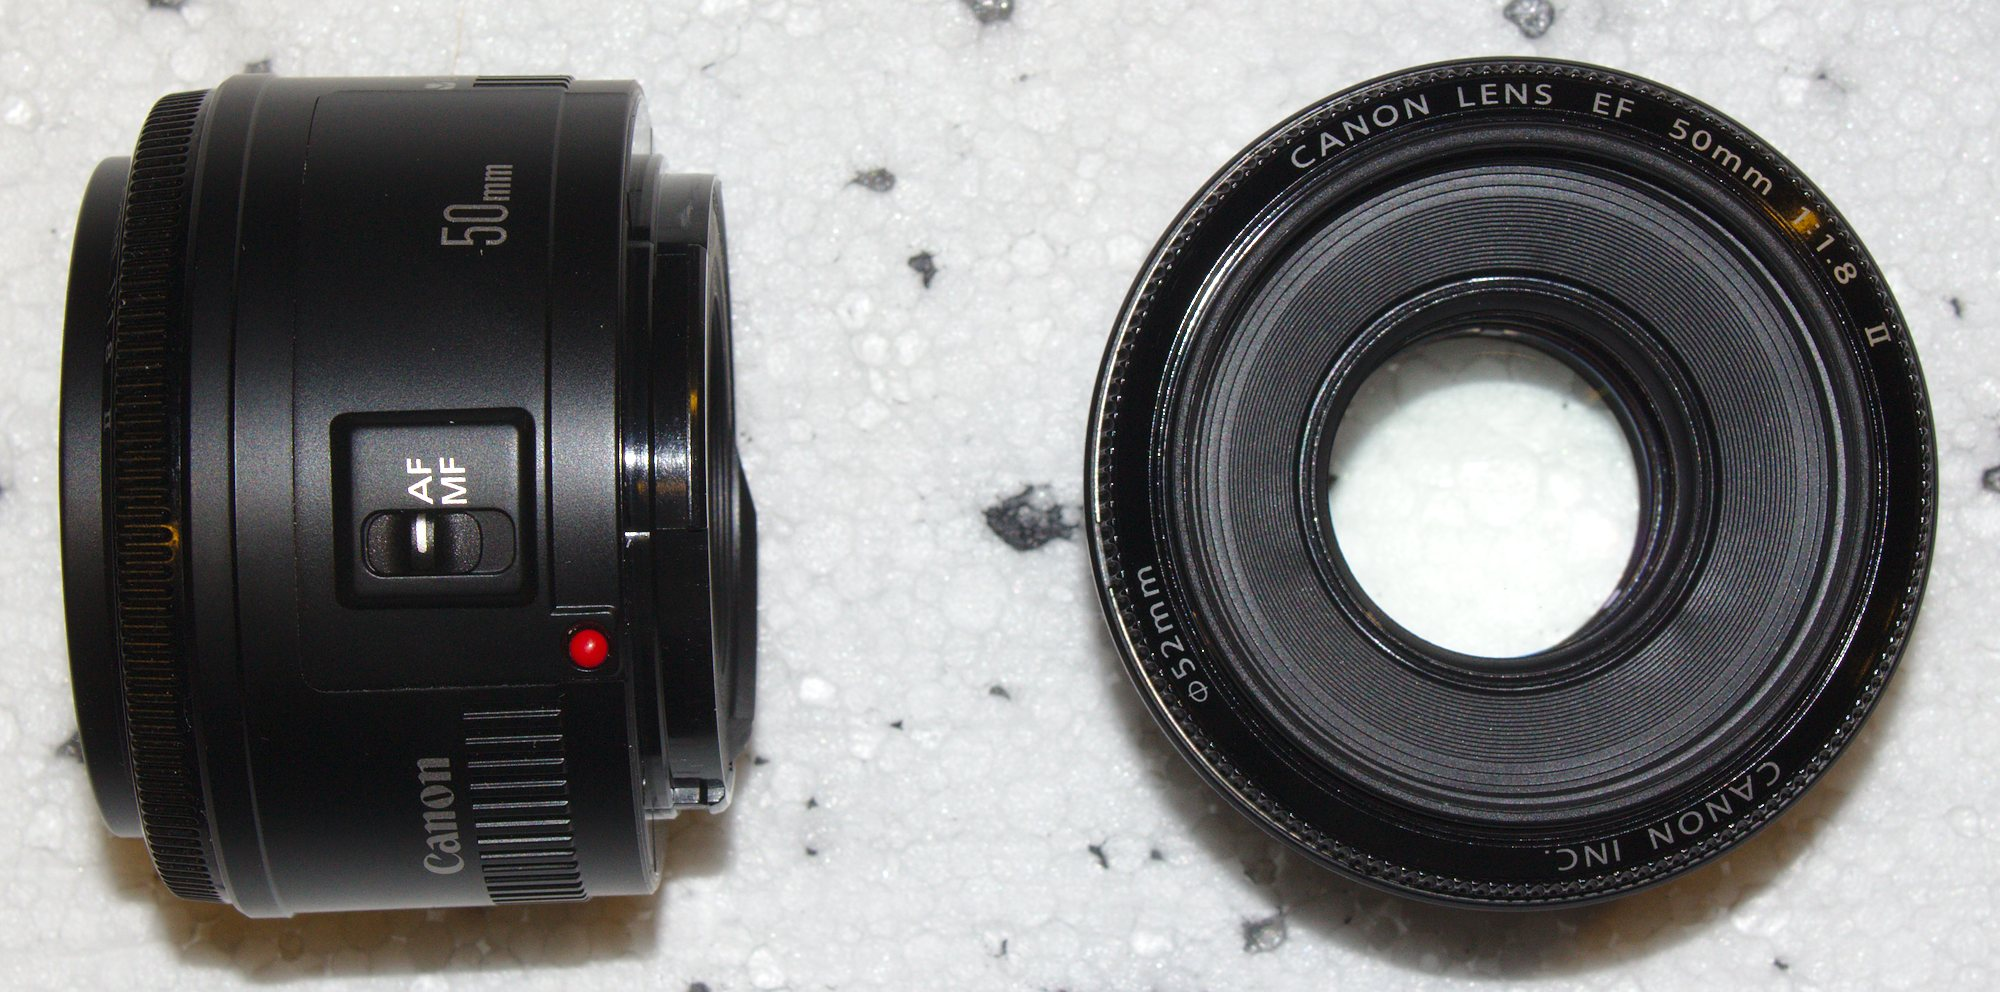
\includegraphics[width=0.8\textwidth]{canon50mmlens}
%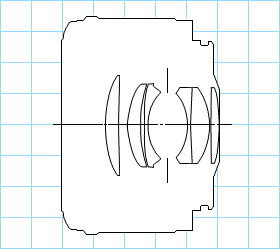
\includegraphics[width=0.4\textwidth]{canonef50mm-2}
}{fig:canonef50mmlens}
{Canon EF 50mm f/1.8 II, a fixed focal length lens with manual focus and autofocus}

\subsubsection{Magic Lantern}

An important consideration was the ability to use the third-party Magic Lantern (ML) firmware add-on;
it was originally developed for tools and improved user interfaces for video recording, but has been extended for numerous other features too.
It was installed on each camera in the rig.
Firstly, it provides experimental support for raw video recording, easier remote triggering for video, and other hacks;
additionally, being open source, it can be modified for any custom purposes, such as multi-camera synchronization aids, if necessary.
It is a separate native program for the ARM-based DIGIC processor, and runs in the camera alongside the original firmware, loaded from the memory card, using the same operating system and configuration menus. \cite{magiclantern}
A screenshot of a menu grid displaying some of the additional functions is shown in Figure \ref{fig:ml-menu}.

ML is installed on a memory card, and it does not make permanent changes to the camera's original firmware.
Still, being third-party software based on reverse-engineering efforts, there is a small risk of unexpected instability.
ML has an active user forum, a wiki, and an automatic software build system for releasing nightly testing versions.
As an open source project developed in a distributed fashion, it suffers from inconsistent documentation and coding style, and is occasionally best examined by reading source code, written in the C programming language.
No stable release is offered for EOS 700D yet, but the unofficial testing version has been long in use by the community. \cite{magiclantern}

\simplegfx{h}{0.6\textwidth}{ml-menu}{
	Magic Lantern grid menu in movie mode, showing a subset of its features.
}

% }}}

\subsection{Hardware construction} % {{{

The cameras need additional support structures for mounting.
A trivial solution would be a tripod for each camera, which would not allow stacking the cameras vertically, though.
Two main methods were considered; they are described below.

\subsubsection{Mechanical options}

With flexibility and mobility as requirements, the system should be built of removable parts that need no modifications to the environment, such as screwing bolts to nearby walls.
The separate parts should be small enough for transportation, but large enough for rigidity and build simplicity.
Each camera should be able to turn at least in landscape and portrait mode to fully utilize the picture frame for portrait subjects, such as human faces.

Two different major designs were considered: a hinged frame consisting of industrial aluminium profile system, or individual tripod stands available in most photography stores meant for supporting audiovisual equipment.
For connecting the cameras, a custom profile could make use of also custom built parts; also, photography stores sell screws and clamps meant for connecting cameras, lights and other hardware.

Extruded aluminium profiles such as those by MiniTec, Item or Bosch Rexroth consist of rectangular tube with a T-shaped slot running along each side for screws, sometimes called T-slot systems.
%The profile systems are commonly used in assembly lines and other automation installations in factories, but also in smaller assemblies
Mechanical dimensions vary by manufacturer but most supply a large catalog of connection brackets, hinges, screws etc.\ that allow much flexibility in the frame design.
A hobbyist-purposed manufacturer OpenBuilds targets open source projects, such as 3D printers and CNC routers.
The cost of such profile is around 10-20 EUR/m, with varying prices for connection pieces; availability varies by supplier.

Ready-made light or speaker stands come in a variety of sizes and share a common design with an extendable center rod and three legs.
Typical light stands have an universal mount in top end of the rod for fastening a lamp.
Speaker stands typically share a similar standard; in general, they are also heavier and thicker to support a larger mass.
Most photography and audio/video studio stores offer a variety of light and speaker stands.

A custom aluminium profile system would have its benefits in rigidity and positional flexibility, because it could be built in any shape.
On the other hand, one rigid shape is more difficult to modify when such a change is needed.
Standard light or speaker stands are attractive because of their availability in normal stores.
They also can be moved around, which also means more work in configuring the camera poses again.
A stand consisting of mostly round rods lacks flat surfaces and slots that could be used for fastening parts together.
For that purpose, special clamps and ball heads are sold separately.

Machine vision cameras do not generally use the same tripod screws aimed for consumer market, but are screwed on the frame with custom bases.

\subsubsection{Selected design}

The method of choice was to use ready-made, heavy duty lighting stands.
Millenium LST-310 (a brand by the Thomann music equipment store \cite{thomann}) is a sturdy three-legged lighting stand with a pole that can be extended several meters high.
Additionally, it has a rotating horizontal bar at the top.
Similar tripods were used in other projects in the same laboratory and they were found useful and rigid.
The relatively heavy weight (10 kg) makes the support structures steady. % FIXME weight
Four of these stands were bought, which should allow a moderate coverage around a subject. %and testing was done mostly with three, with three cameras in each.

For flexibility, each camera should be able to rotate in at least to horizontal or vertical pose, with arbitrary aiming position.
Manfrotto 494 ball heads were used for this purpose, connected to the tripod rod with Manfrotto 035 Super Clamps.
Figure \ref{fig:camconnection} shows a complete connection from a stand pole to a camera.

The total structure of all nine cameras divided in three supports (Figure \ref{fig:totalsetup}) takes up relatively little space, and is flexible enough to set up around any human-size subject or smaller.
The stands can be carried in bags and the more fragile parts are fitted in two cases shown in Figure \ref{fig:cases}.

Wires and power adapters are fastened to the stand legs in long-term use to reduce wires running on the floor.

\simplefig{h}{%
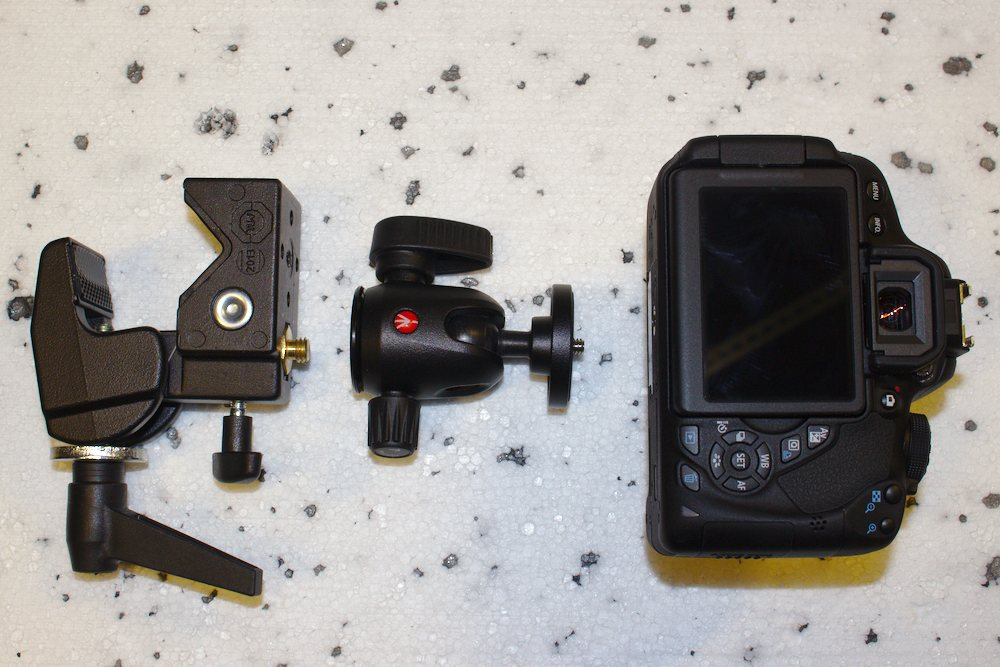
\includegraphics[width=0.45\textwidth]{connparts}
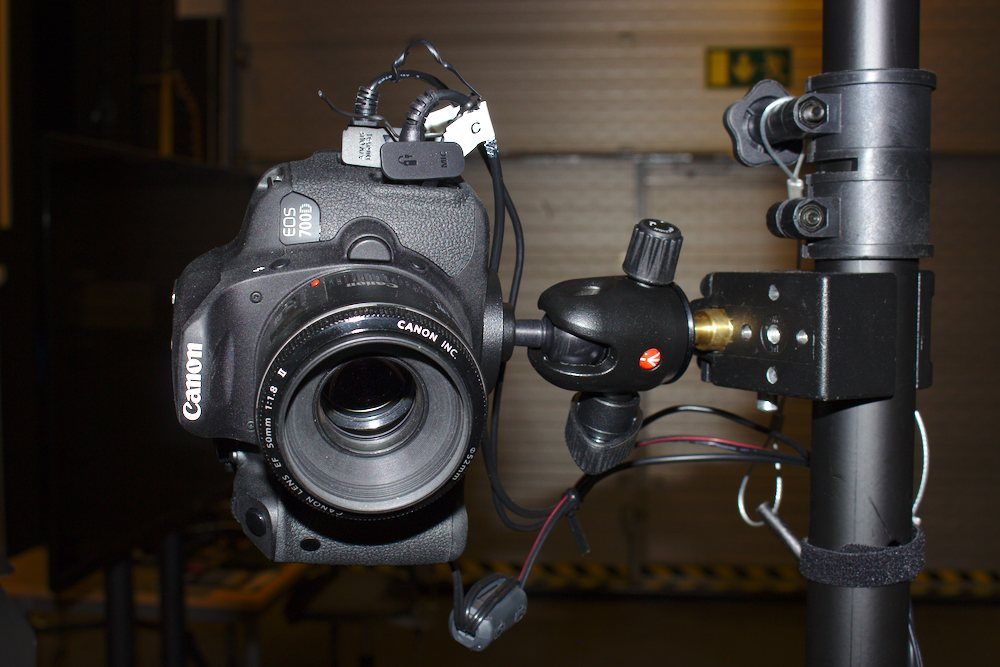
\includegraphics[width=0.45\textwidth]{camconn}
}{fig:camconnection}{
	Left: the Super Clamp, ball head, and a camera separately.
	Right: one camera connected to a pole and its wires.
}

\simplegfx{h!}{0.8\textwidth}{totalsetup}{
	Complete setup with cameras and spot lights for video recording.
}

\simplegfx{h!}{0.8\textwidth}{cases}{
	The fragile parts of the system fit in two equipment cases padded with soft foam rubber.
}

\subsubsection{Lighting}

An even lighting is necessary to capture the subject properly, as described in Section \ref{sec:bg-lighting}.
Unwanted lighting artifacts include harsh shadows and sharp reflections.
Most shadows affect the scanned colors in an unwanted way, since the subject is to be relighted in a digital environment where shadows are formed artificially by calculating the brightness in every illuminated pixel separately.
Sharp reflections make reconstruction harder, since the position of the reflection depends on the viewing direction, making the appearance of the surface different in different views.

In still photographs, flash units bounced from white objects are a practical way to achieve a good lighting.
Typical flash units are either bounced away from white umbrellas sold for this particular purpose, or shot through a large and semitransparent cloth.
For video recording, either a continuous light source or a high-frequency stroboscope synchronized to the video frame rate would be needed.
Since the selected cameras do not support frame synchronization, a continuous light is necessary.

In the scope of this work, no lights were purchased, as readily available flash units and spot lights in the workplace could be used temporarily to evaluate the amount of light needed.
Two standard flash guns attached to the cameras were used for still photograph samples, and three studio spot lights were tested for video recording.
Detailed description on the lights is given in Section \ref{sec:samplesubjects}.

% }}}

\subsection{Remote shutter synchronization} % {{{

For a rig with possibly non-static subjects but an intended result of a still subject, the cameras have to be synchronized to record the subject at the same instance in time.
Photo synchronization was done with a remote mechanism provided by the camera, by driving the remote control of all cameras simultaneously.
However, a short light pulse of a flash unit typically synchronizes the cameras if the surrounding environment is dark, and the camera shutter synchronization has less strict requirements.
In video recording mode, the same remote wire can be used with 3rd-party firmware to start recording.

% }}}

\paragraph{Canon remote trigger}

The selected Canon EOS 700D has an input port for focus trigger and shutter release, in addition to the integrated focus and shutter button.
The camera uses a standard 2,5 mm stero jack for connecting external remote controllers.
Wired and wireless electronic remotes are available in the market, but no standard devices for triggering several cameras arbitrarily are well available; some expensive wireless devices advertise support for multiple cameras using one shutter release, with no well defined latency.
Fortunately, the triggering method is widely researched among hobbyists; it is well enough documented in the internet.

The remote release jack is a three-contact connector, where one pin serves as a common ground, and connecting another pin to the ground triggers the camera's autofocus and metering, and the third pin releases the shutter when connected to the ground. \cite{docdiy}
The pins supply some current that flows back to the camera via the ground pin.
It is safer to separate the cameras from each other electrically instead of connecting the similar remote wires of all cameras together.
A commonly used method among the DIY community is to use opto-isolators to control each camera individually, isolated from the shared control circuit.

\paragraph{Isolation}
An opto-isolator provides a galvanically separated switch that can be used to electrically ``connect'' the release wire to the camera's ground such that no electrical signal path is shared between the cameras.
The switch is a phototransistor that is triggered externally by the light transmitted from a light emitting diode (LED).
Both the phototransistor and the LED are installed in an opaque plastic housing.
As an example, the opto-isolator device used in this work is shown in Figure \ref{fig:singleopto} next to the circuit it was used with.
The particular device works in open collector setting, exposing the collector pin that is left unconnected (``open'') and the emitter pin of the transistor.
Another common setting is a powered device that outputs a voltage signal from a power supply.

\subsection{Universally synchronized multi-trigger} % {{{

By connecting each camera to a separate opto-isolator and driving all of them from same source, all cameras are triggered simultaneously in a safe fashion.
To fully automate the system, the trigger device should be connected to the computer that downloads the photos from the cameras.
Additionally, the cameras are enabled to shoot separately in addition to the synchronized simultaneous mode.

An alternative method in synchronization could have been one third-party wireless remote trigger per camera;
however, they are expensive (approximately 100 EUR per transceiver), may be not as consistent as a wired solution, and would require modifications to work connected to a computer.

Custom, undocumented solutions previously used for hard synchronization for MV cameras by e.g.\ Bickel et al. \cite{bickel2007multi} include ready-made USB I/O boards such as those provided by \cite{datatranslation}

\subsubsection{Microcontroller platform}

A microcontroller (MCU) is a tiny computer in a single, usually fingernail-sized package containing a microprocessor core, RAM, nonvolatile program memory and peripheral devices; all parts required to run a single user-defined embedded application typically with no general operating system.
The Arduino microcontroller board is a popular example.
The typical programming languages for microcontrollers are C and C++.
Communication on the host PC end of an USB connection, when supported, can be implemented in any language.

In this work, a microcontroller prototyping platform called Nucleo-F401RE by STMicroelectronics \cite{stnucleo} was used.
This platform has a built-in USB port for simple communication.

A MCU was chosen over e.g.\ a computer-controlled relay board because of its customizability and low price.
On one hand, such a device is more complicated to set up than a simple switch, but on the other hand, it can be programmed to sequence the cameras in any arbitrary order.
It can also be used to measure the shutter delay and the actual precise time when each camera takes the picture; each has small unpredictable variations.
When capturing moving targets, measuring this lag variation could be of interest.

\subsubsection{Hardware}

\simplegfx{h}{0.6\textwidth}{nucleo}
{STM32 Nucleo-F401RE microcontroller development board.}

The Nucleo-F401RE (Figure \ref{fig:nucleo}) is a prototyping board designed around the STM32F401RET6 microcontroller IC.
This MCU contains a relatively powerful 32-bit ARM core, space for 512 KB of program code, 96 KB of RAM, 51 general-purpose I/O pins available on the board, and other peripherals such as timers and analog/digital converters.
A single-wire debugging (SWD) method is supported to debug the running software in real time. \cite{stnucleo}

The trigger was constructed for ten cameras, functionally transferring trigger pulses from a PC to all cameras synchronously through opto-isolators and 2,5 mm stereo cables connecting to the cameras.
For each output, a Toshiba TLP621-2 dual opto-isolator was used, mainly because they were readily available; any similar device would work.
An output pin in the microcontroller drives an LED of the isolator, making the corresponding transistor conductive.
Schematic of one camera controller is shown in Figure \ref{fig:singleopto}.
Each LED is driven through a current-limiting resistor of 220 ohms, resulting in about 10 milliamps of LED current with the LED voltage drop of 1.15 V specified by Toshiba datasheet, matching the specified test condition in the datasheet. \cite{tlp621}
This results in the transistor conducting the current in the camera remote connection.
The cameras have shown to consistently respond to this well.

The circuit was initially constructed on a solderless protoboard, ``breadboard'', shown in Figure \ref{fig:camsremote-proto}.
After proving that the circuit worked, a proper circuit board was built and installed in an extruded metal enclosure.
Board layout is shown in Figure \ref{fig:triggerboard} and the built case without final lid in Figure \ref{fig:camsremote}.
Full schematic for the whole circuit is available in the Appendix \ref{app:fullschematic}.
The circuit was drawn with the Cadsoft EAGLE, a pcb design software \cite{eaglepcb}; complete schematic and layout files are available in \url {http://github.com/sooda/thesis}.

The circuit board was designed to fit in a recycled enclosure that has inside dimensions of exactly 5 by 3.9 inches (approximately 127 by 99 mm).
The used housing has a removable lid, but any box with a height of 1.4 inches (35 mm) or more should fit.

%\simplegfx{p}{0.8\textwidth}{singleopto} % TODO: disconnect ground from the camera side
\simplefig{h}{%
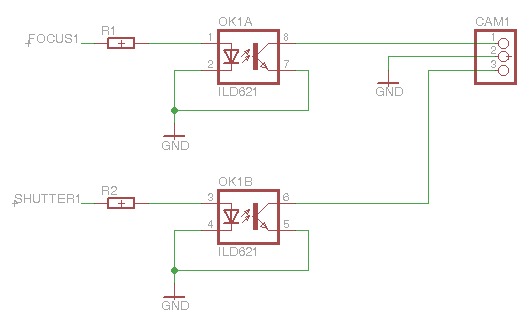
\includegraphics[width=0.5\textwidth]{singleopto}
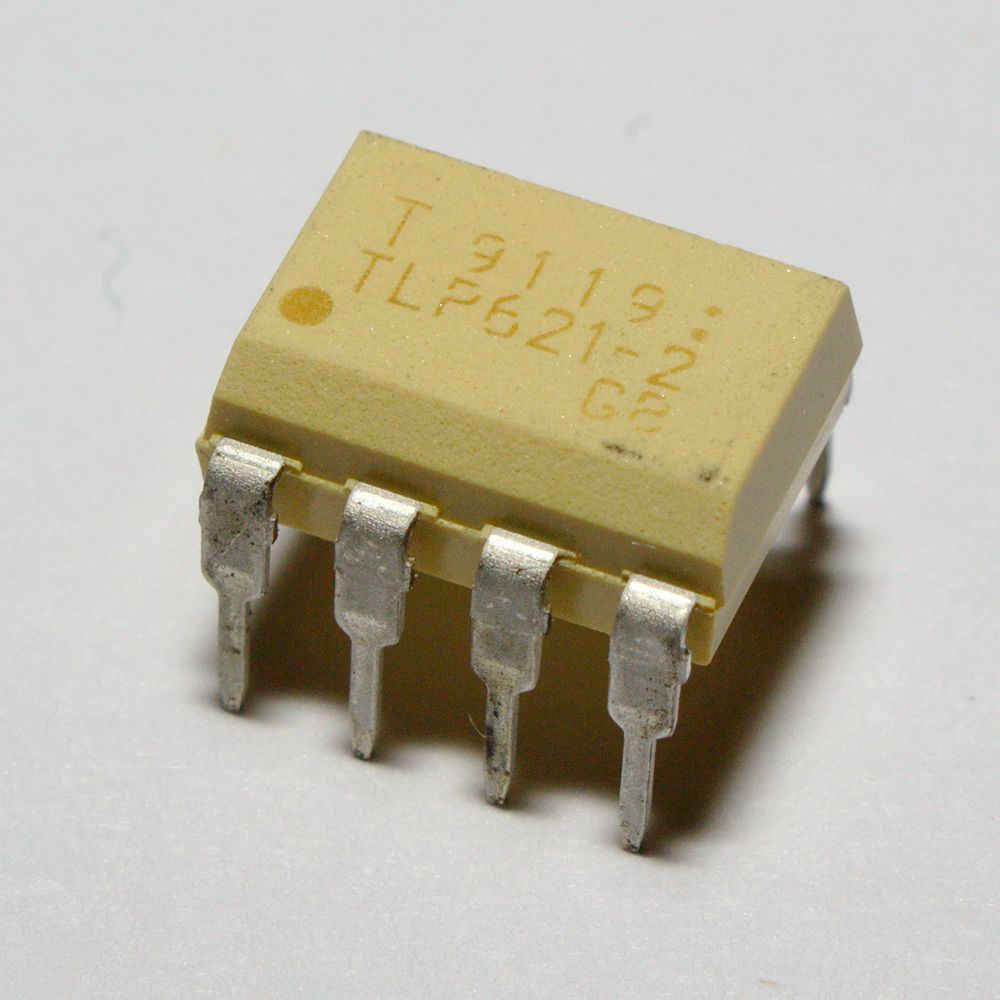
\includegraphics[width=0.3\textwidth]{tlp621-2}
}{fig:singleopto}{
	Left: schematic diagram for a single opto-isolator pair for shutter and focus of a camera, including the current-limiting resistors and a pin header connector for the camera signals.
	Right: TLP621-2 dual opto-isolator in a DIP8 through-hole package, with physical dimensions of approximately 10 by 7 mm.
}

\simplegfx{h}{0.8\textwidth}{triggerboard}{
	Final version of the printed circuit board layout for the trigger box.
	Full schematic is available in the Appendix \ref{app:fullschematic}.
}

\simplegfx{h}{0.8\textwidth}{camsremote-proto}{
	Remote trigger tool prototype on a solderless breadboard.
}

\simplegfx{h}{0.8\textwidth}{camsremote}{
	Remote trigger tool in a case, with lid removed.
	The left side includes buttons, indicator lights and a USB connector; the camera connectors are on the opposite side.
	The microcontroller board is attached to solderless connections, so that it can be removed later for testing purposes if necessary.
}

\subsubsection{Code}

STMicroelectronics advertises the Mbed programming environment and library for the board as an option for writing software for the MCU. \cite{mbednucleo}
The toolchain that compiles the binary for the board works also via the browser in a cloud service, but the libraries can be also installed locally.
All MCU-side code was developed using the Mbed libraries, built locally with the GCC-ARM Embedded toolchain \cite{launchpad-gcc-arm}.
Mbed hides the hardware complexity of the platform, making the total application source code small (less than 200 lines of C++) and relatively independent of hardware initialisation details.
A significant advantage in this hardware abstraction is that a novice could extend the program without previous knowledge on the particular hardware architecture.

The MCU software, or \emph{firmware}, communicates via a serial line that the board passes through USB as a standard virtual serial port, requiring no special drivers.
Communication protocol consists of flags for setting focus or shutter mode and entering bit flags that describe what cameras should be affected, in text mode.
The device echoes the sent characters back, making it convenient to test with a serial console.
The protocol is described in detail in Table \ref{tab:triggerprotocol}.

The code also monitors the Nucleo's integrated general-purpose pushbutton that is used to focus and trigger all cameras simultaneously.
One press focuses all cameras, and subsequent presses send a short shutter signal.
The reset button resets the whole microcontroller, restarting the program with no focus or shutter signals selected.

\begin{table}[h]
	\centering
	\begin{tabular}{l l}
		Set focus pin state & Fxxxxxxxxxx\\
		Set shutter pin state & Sxxxxxxxxxx\\
		Reset all to unpressed & R\\
		Example: push down focus on first and third & F101\\
	\end{tabular}
	\caption{
		Remote trigger protocol; the letter x signifies a single bit (digit 0 or 1) and can be omitted from the start, in which case it is assumed 0.
		Note that the messages set the whole button state instead of sending ``keypresses'';
		to emulate a full keypress, the state must be set first to 1, followed by a set to 0 or a reset.
		Each command must be finished with a space or newline character.
	}
	\label{tab:triggerprotocol}
\end{table}

The used Mbed library does not actually turn all pins on at exactly the same time but in fast succession.
This is not a problem because of the high clock speed of the processor;
the difference between first and last pin changes was measured to be a negligible 1,6 microseconds.
%Expected variance from each camera is supposed to be orders of magnitude longer.

Control software for the host PC was implemented as a small command-line Python script communicating to the virtual serial port of the Nucleo board.
The host controls the trigger's outputs individually, normally driving all the outputs at once.
Sequential or other forms of triggering are possible, because the cameras are controlled individually in hardware.
For example, as each camera is able to record five full-resolution frames per second in burst, interleaving the nine cameras results in short 45 FPS full-resolution imagery.
Also, when using the internal pop-up flashes in the cameras, they can be fired separately to circumvent issues in lighting synchronization or exposure control.

The same MCU can be reprogrammed with another firmware at any time; it was used also for measuring shutter delay of one camera, see Section \ref{sec:shutterdelaymeas}.

The programs are available in \url {http://github.com/sooda/thesis} with source code.

% }}}

\subsection{Custom camera control software} % {{{

% breeze systems $129 per cam
% smartshooter

% FIXME clumsy
% esper design etc.
%General parallelized image acquisition from a large set of cameras has not yet established such a state that general purpose software would be easily available.
%Commercial solutions probably exist, but they are often strictly bound to a specific hardware, expensive, and inflexible.

Some custom techniques were used to preview images of all cameras simultaneously, configure the settings of each concurrently, and retrieve the captured images from them in order.

Like the MCU board layout and firmware, all programs and their sources can be downloaded from \url {http://github.com/sooda/thesis}.
The programs have been verified to work under recent Linux and Mac OS X systems.

% }}}

\subsubsection{Camera control library} % {{{

\paragraph{Camera libraries}
gPhoto2 \cite{gphoto2} is a well-known free and open-source application and library in the C programming language for controlling digital cameras on Unix-like operating systems, supporting over a thousand cameras.
The software consists of a command-line control tool of the same name, \emph{gphoto2}, and a library API, \emph{libgphoto2}.

Instead of relying on each camera manufacturer separately for a software development kit, gphoto2 abstracts common operations behind the same interface.
For example, Canon and Nikon, some of the biggest camera manufacturers, both provide SDKs for controlling their devices remotely via a USB connection from Windows and Mac OS X. \cite{canonedsdk} \cite{nikonsdk}
Sony provides an SDK for Android and iOS. \cite{sonysdk}
Olympus has had an SDK, but it is no longer available. \cite{olympussdk}
To support all vendors, one would have to write code for all APIs.
In this work, extendability to other vendors was seen as an optional advantage.
In addition, development kits provided by the vendors may be more restrictive and may not be fully available.
%Canon provides a Digital Imaging Developer Programme that requires registration to be able to download the SDK (EOS Digital SDK, or EDSDK).

Furthermore, the Canon EDSDK claims in the manual not to support sessions to more than one camera in parallel. \cite{canonedsdk}
This technical issue could probably be overcome with additional workarounds in software, though.

Libgphoto2 implements the \emph{Picture Transfer Protocol (PTP)} \cite{ptp} for setting properties and transferring pictures via USB.
Details on list of configurable properties and sequences for capturing pictures and preview vary among manufacturers, and the library has most thorough support for Canon and Nikon cameras.

\paragraph{gphoto2 wrapper}
A ``wrapper'' code library was written in C++ for libgphoto2 to automate memory and resource management, simplify the usage of the raw library, and to write the programs themselves in clean C++; libgphoto2 itself is implemented in the C language and is not well documented.
Libgphoto2 exposes the data as objects, and the wrapper simplifies their handling and implements some more complicated operations, such as creating a new camera object instance, configuring parameters, and downloading preview frames and actual shots.
The library itself is also not thread-safe: if a camera is used in to threads of execution simultaneously, unexpected errors happen. \cite{gphoto2}
Locking mechanisms were written for the wrapper to prevent more than one executing threads from accessing a camera instance simultaneously.
The library initialization was also protected, because it loads camera-specific sub-libraries only after first use; if many cameras are tried to initialise at the same time, another error would occur.

The wrapper is written exclusively with libgphoto2 in mind, but as it actually hides the implementation details strongly, it could be ported to use e.g. EDSDK without affecting the actual applications using it.

% }}}

\subsubsection{Previewing} % {{{

\simplegfx{h}{1.0\textwidth}{gphotogrid}{
	A custom program, \emph{gphotogrid}, was written for displaying a preview feed of many cameras in a grid and configuring exposure time, aperture, and ISO sensitivity jointly for all cameras.
	New settings are easy to add if needed.
}

\simplefig{h}{%
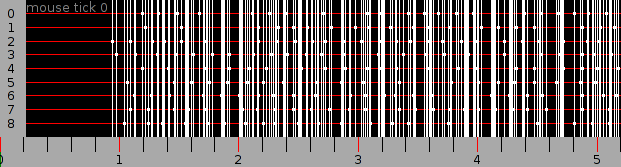
\includegraphics[width=\textwidth]{timeline-nosync}
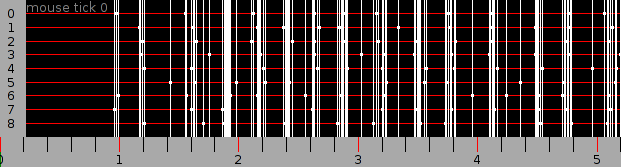
\includegraphics[width=\textwidth]{timeline-sync}
}{fig:grid-timelines}{
	Timelines displaying the points in time (x axis, in seconds) when frames have been captured from different cameras (y axis, by camera number).
	The upper image shows all cameras running freely, and in the lower image, no new frame is captured from any camera until all have finished the current capture.
}

Although each camera can be positioned by individually looking through the viewfinders, a simple preview live feed is almost mandatory to properly set up a new configuration to see the big picture.
A preview matrix of all cameras makes it easy to identify the cameras and to see if they all have been pointed to correct directions, and to verify that their settings are the same by judging from the image quality.
The program is shown in Figure \ref{fig:gphotogrid} and is found in the github repository under the name \emph{gphotogrid}.
It is written in C++ and uses the libgphoto2 wrapper for camera control and the wxWidgets GUI library \cite{wxwidgets} for the user interface.
The purpose is to view the picture frame of each camera in realtime and change the most important camera parameters concurrently.

\paragraph{Preview stream}
Libgphoto2 provides an interface for reading a camera preview frame at a rate of several frames per second, speed depending on USB hardware performance, the number of cameras used in parallel because of USB bus limits, and CPU processing power as the images are resized to the screen.
A preview feed is connected to each camera to download the frames as fast as possible, and the user interface displays them as a grid, with configurable camera order.
Because libgphoto2 does not offer asynchronous image or configuration transfers, a new thread of execution is set up for each camera, and the preview pictures are transferred to the main screen via concurrency-safe queues in the application itself.
The code control flow is described in a simplified form in Listing \ref{lst:gphotogridalgo}.

% FIXME this to experiments?
\paragraph{Timeline}
A timeline widget was also developed to investigate the points in time when the preview frames have been grabbed, aiming to study synchronization accuracy using this preview method.
Observing the times was found to be of no use, because the pipeline from camera to application seems to be so complex that the preview frame rate is completely sporadic, with no ability to control the frame order or timing.
The application includes a checkbox for ``synchronizing'' the preview grabber threads so that no camera starts to read a new preview before all have read the last frame.
This synchronization attempt did not have any positive effect; in contrast, restricting each camera this way made the performance much worse, as can be seen in Figure \ref{fig:grid-timelines}.
In the figure, a vertical bar is drawn for each frame captured, with a small circle on the line of each corresponding camera number.

\paragraph{Identification}
The cameras are identified and ordered by a name written to the configuration set under a property called \emph{artist}, found at least in Canon DSLRs.
The artist name can be set either via USB or from the camera's physical user interface, and it is supposedly originally meant for writing the camera owner's name in the image file's metadata, along with copyright information.
For the camera rig, a single letter was used for each camera, ordered from \emph{A} to \emph{I}.
A separate configuration property stored in the camera itself is most robust; USB port name can be used as an alternative to identify the cameras, but the port name changes when the cameras are plugged in another way when rebuilding the rig or using another computer.

The pop-up flashes should not be activated during use, because the camera was found to ignore the effects of most settings when the flash is up.
Additionally, remote control disables the camera user interface.
Taking pictures or changing settings is not possible while previewing.

It is recommended to spread the cameras as evenly to all USB root hubs as possible to help even out the transmission capacity, maximizing the frame rate.
The same is recommended when downloading the actual images.
The USB hub where a device is connected can be verified in Linux by looking at the output of the \emph{lsusb} command-line tool.

\begin{lstlisting}[
	caption=Pseudocode for \emph{gphotogrid}.
	The lock task runs only if synchronization is enabled.
	The asynchronous UI settings are not shown.,
	basicstyle=\ttfamily\footnotesize,
	label=lst:gphotogridalgo,
	float=h
]
per-camera preview feed {
	while running {
		download preview frame
		record current time
		push frame and time to queue
		if sync enabled {
			notify lock about finish
			wait for next round from lock
		}
	}
}

locking task {
	while running {
		wait for all frames
		notify loaders for next round
	}
}

screen update requested {
	for each camera {
		each queued frame {
			store frame time to timeline
			count number of frames
		}
		scale last frame to screen
	}
}
\end{lstlisting}
% }}}

\subsubsection{Configuration} % {{{

Remote control of all cameras is required to set all settings, such as shutter speed, jointly from the same computer instead of clicking on each camera's buttons manually.
The preview matrix program allows to change exposure time, aperture size and ISO sensitivity, but more tools were written for automatic configuration.

The following small command-line scripts were written using the gphoto2 command-line tool:

\begin{itemize}
	\item \emph{config}: reset common parameters to defaults for all connected cameras, listed in the script itself
	\item \emph{forall}: run gphoto2 with the user supplied arguments for all connected cameras serially
	\item \emph{forallp}: as forall, but in parallel, saving time
	\item \emph{post-download-by-camid}: download all previously shot files stored in the cameras to directories named by camera artist name
	\item \emph{readconfig}: read and copy settings from one camera to all others currently connected
	\item \emph{release-uilock}: unlock the physical user interface of connected cameras by fetching a listing the filesystem; a workaround for the Canon glitch described below
\end{itemize}

The \emph{forall} and \emph{forallp} scripts are trivial shortcuts to autodetecting all cameras and passing commands to gphoto2 for each, and are useful for case-specific problems or e.g. setting individual configurations temporarily.

With \emph{readconfig}, one camera is first configured manually, and the settings are cloned to others automatically with the script.

Either libgphoto2 or the EOS 700D camera has a bug that locks the camera's physical user interface when configuring the cameras and even quitting the program:
it appears that this is a safety feature that is left on after disconnecting the configuration connection, and probably gphoto2 does not release it properly.
When setting or getting any configuration, the camera screen turns off and all buttons stop responding until the camera is rebooted, USB cable is unplugged, or if gphoto2 touches the camera's filesystem.
Listing the files is thus enough and it has no side effects.
The workaround script \emph{release-uilock} was written as a reminder to perform the listing for all connected cameras.

% }}}

\subsubsection{Image acquisition} % {{{

% offloading

A command-line tool called \emph{paraphotos} for downloading the images in realtime in parallel from each camera was developed in C++ using the same libgphoto2 library wrapper.
The cameras send a notification via USB when a new photo is taken with the shutter button or the remote release.
When this new file is found, it is downloaded and named by a running index and camera name.
The user is notified when all cameras have finished for a single shoot;
also, when the program is requested to quit, it first waits until the last pending download is finished.
Each download task runs in a separate thread of execution to overcome the synchronous nature of libgphoto2, as well as the notifying task; a simplified code control flow is described in pseudocode in Listing \ref{lst:paraphotosalgo}.

basic algo without debugprints etc.
ctrl+c breaks the loops
\begin{lstlisting}[
	caption=Pseudocode for \emph{paraphotos}.
	Ctrl-C (interrupt) signal is captured and it requests quit.
	Many possible debug message prints not shown here.,
	basicstyle=\ttfamily\footnotesize,
	label=lst:paraphotosalgo,
	float=h
]
per-camera download {
	while quit not requested {
		poll for event
		if event is file addition {
			download file
			notify ui
			wait for ui finish
		}
	}
}
ui notification {
	while quit not requested {
		wait for the number of cameras events
		notify user about a ready image group
		signal downloaders to continue
	}
}
\end{lstlisting}

Almost the same functionality could have have been achieved with the gphoto2 command-line utility; using the library directly with C++ resulted in cleaner code and probably faster operation.

Video acquisition is not possible in realtime; instead, the video files have to be saved on the memory cards first, and downloaded when the recording is complete.
The \emph{post-download-by-camid} clones the file systems from the cameras to local disk, bringing the video files accessible.

Video format should be set to 720p at 50 or 60 FPS or 1080p at 25 or 30 FPS.
Both resolutions result in a video bitrate of approximately 5 MB/s with default settings.
The video format is H.264 encoded in a Quicktime MOV file, with a stereo audio in raw lossless (PCM) format with 48 kHz sample rate and 16 bits per sample.

The bitrate can be extended from Magic Lantern's menus, but bitrate changes are still experimental code and recording may stop if the camera or the memory card is not fast enough.
Video keyframe rate can also be changed with a development version of ML and probably will be stable in the future;
in the video codec used, the frames can be \emph{I-frames} (intra-frames), with fully encoded data, or \emph{predicted frames}, encoding changes between frames, with less accurate information.
Raw recording is also supported, but with the limited memory card speed, only a low resolution is achievable.

% }}}

\subsection{3D reconstruction software survey} % {{{

% something on individual algorithms/tasks of the reconstruction pipeline; standalone pipelines; web services; sw/hw solutions

When the imagery has been downloaded to a PC, the actual reconstruction can be started.
There is a wide collection of libraries, open-source tools and commercial packages for both automatic reconstruction and generic mesh editing for post-processing the data.
Some of them are presented in this section.
In the scope of this work, new reconstruction algorithms or implementations are not implemented;
thus, it is important to test the rig with readily available implementations.

Many, if not all, programs assume that the Exif data embedded in the photograph files describes the used focal length and sensor dimensions.
Canon EOS 700D stores this information properly in the files.

 % }}}

\subsubsection{Free libraries} % {{{

There exist several generic computer vision and geometry and image processing libraries, most common of them being probably OpenCV \cite{opencv}, Point Cloud Library (PCL) \cite{pcl} and Computational Geometry Algorithms Library (CGAL) \cite{cgal}.
These are written in the C and C++ languages and they have bindings to several scripting languages too.
For future work using the rig, these libraries present a well known basis for developing own tools.

OpenCV contains a large set of utilities for 2D image processing and extends also to camera calibration and 3D reprojection.
It is probably the most commonly known and most used computer vision algorithm package.

PCL contains a set of algorithms for filtering, segmentation, registration, visualization, and more for working on data sets that consist of points that may share attributes such as colors and normals.
PCL is popular in robotics involving three-dimensional computer vision; its algorithms apply well to point cloud data obtained easily using a LIDAR or similar range imaging device.

CGAL provides access to more general and mathematically more geometric data structures and algorithms extending in combinatorics, convex hulls, polygons, arrangements, mesh processing, triangulations, voronoi diagrams, visualization and more, with a more mathematically rigorous approach.

% }}}

\subsubsection{Free programs} % {{{

While libraries can be used to write new tools, many pieces of software are readily available that implement 3D reconstruction based on methods presented in Section \ref{sec:static3d}, and are distributed in source code form and/or readily usable binary executables.
Some of the most known state-of-the-art implementations are listed below.

Camera Calibration Toolbox for Matlab, also included built-in in OpenCV, is a more or less standard tool to single-camera and stereo camera calibration.
The toolbox computes undistortion maps and intrinsic and extrinsic parameters with checkerboard images using non-linear optimization and planar homographies. \cite{camcalmatlab}

Bundler is a bundle adjustment and structure-from-motion system for computing camera poses and sparse point clouds, targeted for large-scale unordered photo collections, originally used for the Photo Tourism project. \cite{snavely2006photo}

SiftGPU is a fast SIFT implementation for graphics processing units (GPUs) by Chenchang Wu. \cite{changchang2007siftgpu}
It is built on Sift++ \cite{vedaldi2011sift++}; both are based on difference of gaussians, a method for edge detection. \cite{marr1980theory}

Multicore (parallel) bundle adjustment PBA is a fast bundle adjustment library built with the modern parallel nature of multi-processor computers in mind. \cite{wu2011multicore}

Patch-based, multi-view stereopsis (PMVS) starts from a set of matching keypoints (features) and a pre-acquired camera calibration, and expands the keypoints to a dense patch set iteratively, resulting in a high number of oriented points.
PMVS is usually combined with CMVS, a clustering tool that decomposes the input set to smaller clusters that are more convenient to process, when the amount of different views is large. \cite{furukawa2010accurate,furukawa2012patch}
% xxx viewpoint invariant patch, repetition analysis http://www.academia.edu/2021718/3D_Digitization_using_Structure_from_Motion
% xxx2 graclus, wat pba

VisualSFM \cite{wu2013towards} is a common and free but closed-source full-scale pipeline that implements a structure from motion algorithm and simplifies the workflow of several external programs, finally visualizing the results.
The needed external tools are feature matching, bundle adjustment and dense reconstruction.
VisualSFM is probably the most common tool in the open source and research community for practical use.
It integrates into a few clicks the pipeline from images to 3D point cloud, using SiftGPU for features, its own radial undistortion model and SfM for camera estimation, PBA for bundle adjustment, and finally PMVS/CMVS for dense matching.
A common final step is to use Meshlab to filter outliers away from the data and to build a triangular textured mesh of it with the input points and normals.
%PMVS is suggested by many others.

Meshlab \cite{meshlab} is a generic interactive editor of point clouds and meshes, implementing many scientific papers.
It can be used interactively and scripted to do the same steps automatically.
In a reconstruction pipeline, it is one of the last processing steps, used for removing outliers or fitting a surface on a point cloud with the poisson surface reconstruction method, and finally projecting the textures to the generated mesh when given the camera parameters in relation to the point cloud pose.
It can also perform registration between point clouds.

(Screened) poisson surface reconstruction, or PoissonRecon, is another stand-alone program as an alternative for surface fitting. \cite{kazhdan2013screened}

Cmpmvs is a multi-view reconstruction software for transforming a set of calibrated image data to a full textured mesh, used in a similar way as VisualSFM but using internally a different method based on graph cuts and weakly-supported surfaces.
\cite{jancosek2011multi}

Python Photogrammetry Toolbox, popular in archaeological fields, combines Bundler and PMVS/CMVS for a full-scale pipeline. \cite{moulon2011python}

%SFM toolkit combines Bundler and CMVS/PMVS.

% }}}

\subsubsection{Commercial solutions} % {{{

{ \color{red} XXX Which list type is better? }

There is a large selection of commercial software available, often accompanied with a 3D scanning device or a complete service.
Some companies offer completely specialized rigs, some sell a scanning device and a general-purpose software alongside it which can be used as standalone and some only sell software, leaving the hardware implementation to the user.
The following short listings review some of the commercial products that use 3D scanning as a key idea.

% FIXME emphasis on differences

The following list includes software-only reconstruction solutions available for purchase, that work as-is for any general input.

\begin{description}
	\item[Autodesk 123D Catch] is a free and popular web-based application for automatic reconstruction; photos are uploaded to a cloud service, and a textured mesh is generated automatically. \cite{autodesk123dcatch}
	\item[Acute3D] Smart3DCapture is targeted for large-scale photogrammetry and cultural heritage digitization. The software is provided as a standalone program and a library, and it is used in Autodesk 123D Catch. \cite{acute3d}
	\item[Agisoft PhotoScan] has two editions, for 3D designers and professional geographic content manipulation; among the geographic features, it is very suitable for multi-view reconstruction in content generation, and has an active forum for its users. It can be scripted with the Python programming language. \cite{photoscan} Photoscan is used e.g. by \cite{ir-ltd}.
	\item[Faceshift] provides a realtime markerless face capture in a feature space that describes virtual muscle and bone movements, using a single camera and pre-trained poses. The software runs currently with a depth sensor such as Microsoft Kinect. \cite{faceshift}
	\item[3DF Zephyr Pro] by 3DFlow is an automatic reconstruction software that takes photographs as input. A free SfM software, \textbf{3DF Samantha}, is provided too. \cite{3dfzephyr}; The company is a spin-off of a university thesis project. \cite{toldo2013accurate,toldo2013towards}
	\item[Pix4dMapper] converts aerial images to geometric surface models for mapping related applications. \cite{pix4d}
	%\item[Trimensional] is a 3D scanner for iPhone.
	\item[Pixel Farm] provides tools for reconstruction, CG integration and match moving (i.e. augmenting live footage with computer-generated imagery). \cite{pixelfarm}
	\item[3D-equalizer] is a multi-platform 3D tracking solution for the visual effects industry, including Python scripting, customer support, and more. \cite{3dequalizer}
\end{description}

In contrast to the above, the following list includes complete systems that are offered as a service or as an addition to a program only.

\begin{description}
	\item[MotionScan] is the technology behind e.g.\ the video game L.A.\ Noire \cite{rockstar2011noire}, developed by CaptiveMotion. It uses tens of cameras to recover detailed structure and is targeted for video game content generation.
	\item[Pendulum Studios] provides a capture system called Alter Ego that integrates with game engines, used in several video games. \cite{alterego}
	\item [FARO] manufactures hardware and provides scanning software for 3D documentation and surveying, and provides a free application for Kinect-based scanning. Many commercial applications are listed, ranging from product development to crime scene analysis. \cite{faro}
	%\item[Fuel3D] is a complete low-cost handheld scanning system.
	\item[Dimensional Imaging ltd.] provides DI3D and DI4D systems and software for static and dynamic surface capture, respectively, used for video games, research and medical applications. \cite{di4d}
	\item[Vicon] is an old motion capture company, producing both both hardware and software for motion and surface capture and listing applications from life sciences to engineering and enterntainment. \cite{vicon}
	\item[3dMD] offers healthcare-focused systems, software and research papers. \cite{3dmd}
	\item[V-STARS] is a product line of Geodetic Systems, which provides systems for industrial photogrammetry. \cite{vstars}
\end{description}
 % / design+integration / system implementation / more custom subsections
% Tulokset / results
\section{Experiments}

% is X? test X. proof: X is ?.

\subsection{Synchronization issues}

Synchronizing the image sources temporally is important for reconstruction algorithms to work correctly.
A synchronized system captures images from all cameras with a reasonably small time difference, so that subject movement does not introduce additional errors.

\subsubsection{Still capture}

Static subjects do not move or change shape.
However, still imagery of e.g. a human head needs at least semi-accurate syncing, because standing still enough is not possible for longer periods (seconds).
Even though the facial pose would not change, the wrong position of the head in a frame would introduce error.
Similarly, capturing e.g. a still image of a moving cloth needs proper synchronization.

For a completely static subject, the cameras can even be shot separately, each using its own integrated flash unit, to minimize shadows for each viewpoint.
When the light direction is almost the same as the camera's view direction, no shadows are possible.

Still capture using the wired remote trigger was analyzed with a moving object.
%A spinning disk with a dial was captured and the images were compared.
%Sample data is shown in figure \ref{fig:spindisk}

\subsubsection{Video capture}

% intro

The EOS 700D does not support an external sync signal for video recording, but relies on an internal clock to sync the frames within a single video file.
It can be safely assumed that the clock speed has little variation, and thus, little drift and jitter occur in the videos.
Recording offset remains an issue;
processing time of each camera from the shutter button to start of first frame varies because of unknown reasons; even though a wireless remote control of the camera manufacturer would be used for starting several cameras at once, the offset is very noticeable.

% what was done

A test was carried out to find variations in the recording offset.
Three cameras were triggered with a Canon RC-6 wireless remote control.
The remote sends a short infrared pulse to a sensor in the front of a camera when a key is pressed.
The camera was set in video mode and it was configured to use the remote release.
%The exposure time was set to minimum, 1/4000 s, to maximise the rolling shutter effect.
%In this mode, the sensor rows are exposed one by one in succession.
When all cameras were recording, a flash unit (Canon Speedlite 420EX) was aimed at the lenses and fired manually several times.

% what happens

A direct light pulse of a flash unit shows up as an over-exposed, completely white video frame, if the whole frame was exposing the image during the light pulse.
Sometimes only part of the frame would be exposed to the flash light as a rolling shutter effect.
Because the CMOS sensor is cleared and read line by line, the time of the flash can be deduced from the first bright line in the image.
The rows are zeroed from light in succession in the same way as a mechanical focal plane shutter moves and exposed until read.
Thus, the flash light's starting time in the video's internal clock is the frame's start time plus the duration that it takes for the rows before the overexposed one to show up:

\begin{align} \label{timingcalib}
t_{Cl} &= t_{Ci} + t_{Cf} \\
&= i_C * F + f_C / R * F \\
&= (i_C + f_C / r * c) * F
\end{align}

where $C$ is a camera identifier, $t_{Cl}$ is camera-relative time for the light pulse, $t_{Ci}$ is the starting time for the frame where the light shows up, and $t_{Cf}$ is the time inside the particular frame.
The frame index $i$ marks the number of the frame in the video file, starts from 0, and there is $F$ = $1/\text{fps}$ time between the frames.
$f_C$ is the first exposed row, $R = r / c$ is the time for a single row to expose, $r$ is the vertical frame resolution and $c$ is a correction coefficient describing the relation of exposure time and frame duration ($0.5$ in this case, referring to 180 degree shutter).
Offset between two cameras $A$ and $B$ is then $t_{Al} - t_{Bl}$.
The timings are depicted in figure \ref{fig:flashtimeline} as a timeline with matching symbols.

For perfectly synchronized videos, the frames would be identical, and time difference calculated with eq. \ref{timingcalib} for each frame would be zero as $i_C$ and $f_C$ would be constants for all $C$.
A typical measurement result is shown in figure \ref{fig:flashtiming}.
Audio recorded by the cameras' internal microphones at the same event is shown in figure \ref{fig:flashaudio}, and the order of flash pulses in the three frames can be verified from the order of the sound emitted by the flash.

\simplegfx{h}{1.0\textwidth}{flashtimeline}
{Illustration on timing calibration of two cameras using a flash light.
The darkened areas represent the exposure times and the red band represents the light pulse.
In this example, $c = 0.5$.
}

\simplefig{p}{%
\setlength\fboxsep{0pt}
\setlength\fboxrule{1pt}
\fbox{
\includegraphics[width=0.3\textwidth]{flashtiming-a}}
\fbox{
\includegraphics[width=0.3\textwidth]{flashtiming-b}}
\fbox{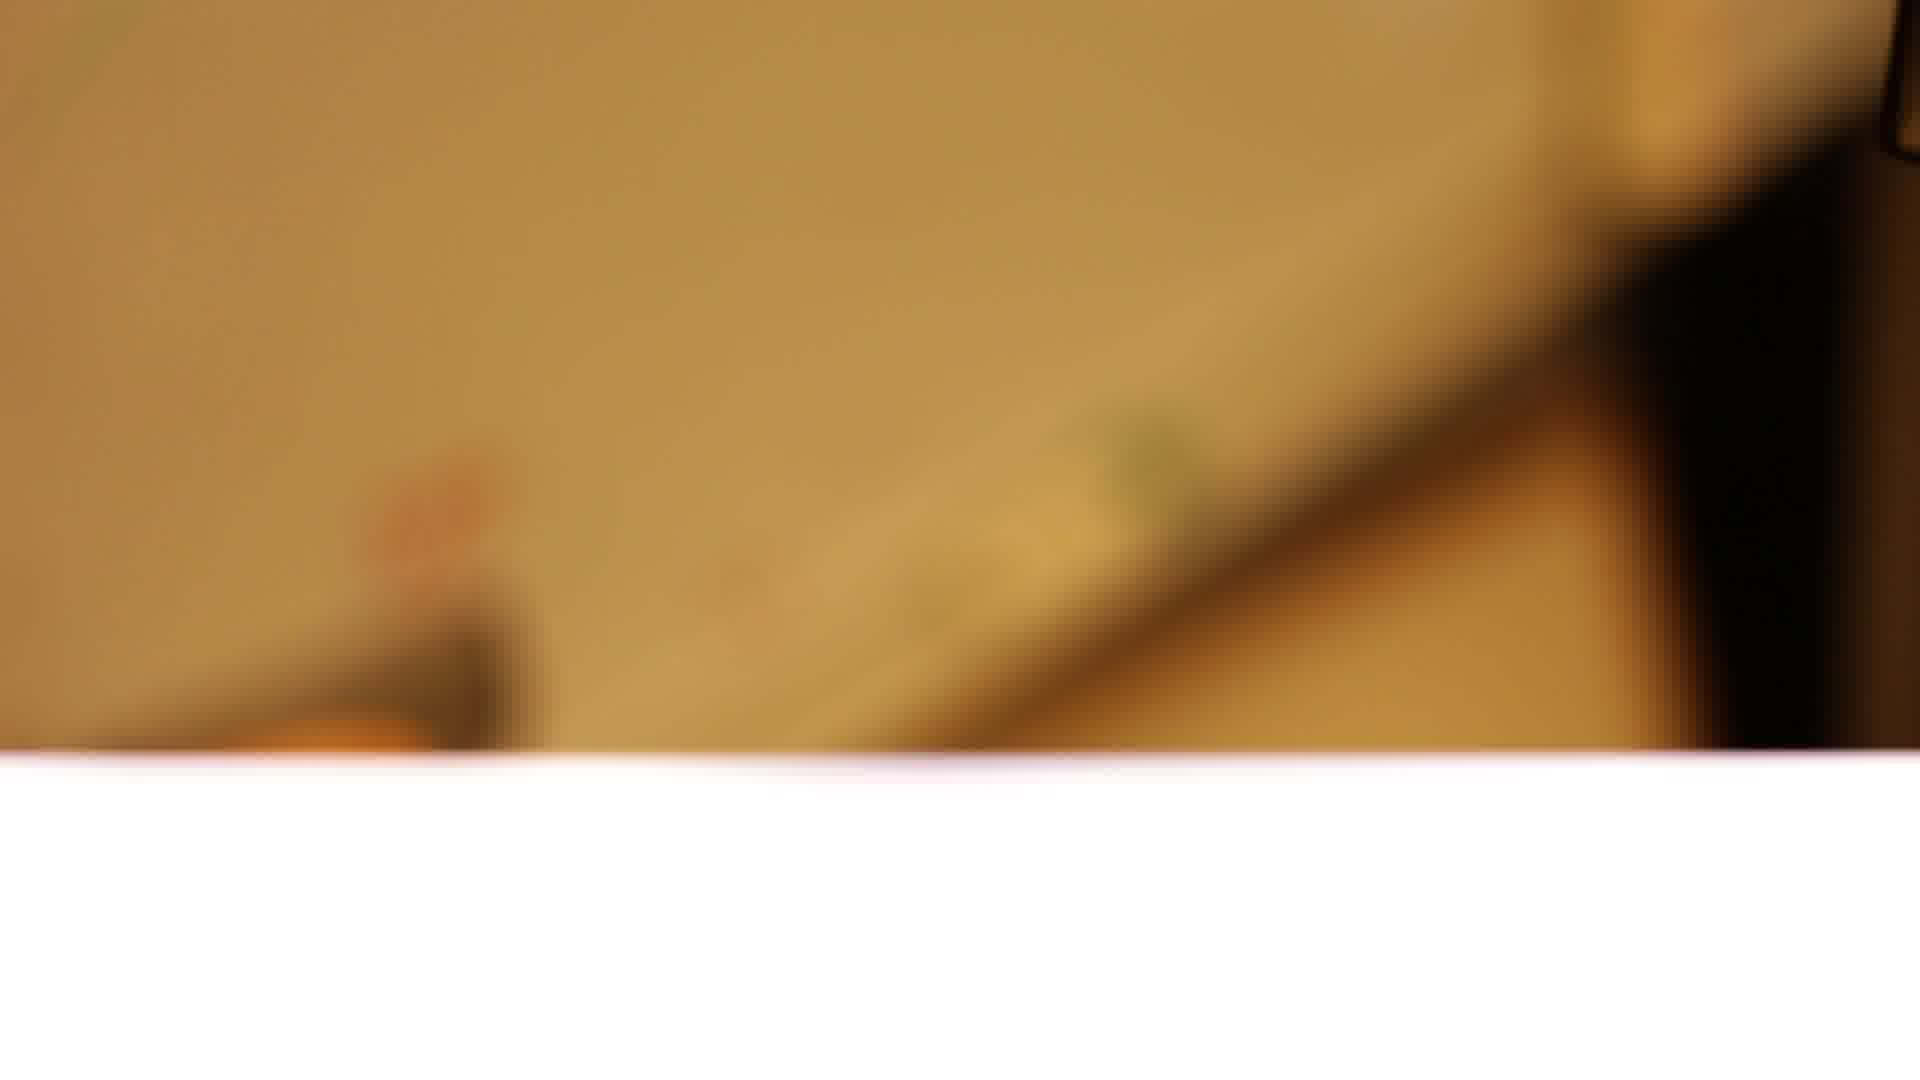
\includegraphics[width=0.3\textwidth]{flashtiming-c}}
}{fig:flashtiming}
{Video frames of three cameras started with the same remote, with the same frame index.
The time for the flash unit to reach maximum brightness is almost instant.
The start of the light pulse can be seen in the leftmost and rightmost frames.
In the middle one, the flash has been fired before the frame exposure started;
the frame before it is still without any overexposed light.
It is impossible to deduce the exact time in this case.
}

\simplegfx{p}{0.8\textwidth}{flashaudio}
{Trimmed audio recordings of the same moment as in figure \ref{fig:flashtiming}, extracted from the video files, in top-bottom order.
First rows of the frames have been exposed at about $t = 0.03 \text{ s}$.
The flash outputs a distinct ``pop'' sound.
}


The method for measuring the synchronization error can be used to calibrate the differences, which aids in artificial sync with optical flow or other methods.
A similar method using the recorded audio is perhaps more familiar, where a distinct sound in the audio tracks recorded by the cameras would be used for calibration.
%The $t_l$ in equation \ref{eq:timingcalib}

Another method for triggering multiple video recordings is to use a ML-based wired remote trigger by pressing the half-shutter, or focus button when a record key has been configured in ML.
This method did not show any improvements in overcoming the offset.

\subsection{Sample objects}

The mask, human heads, legos, books

\subsection{Hard cases}

Low light? Little texture? Speculars? Hair?

% test X. not feasible for X because Y.

\subsection{Accuracy}

\clearpage

\section{Discussion}

%Perf of cloth animation capture

%other uses - street view, autom driving, geodetic systems

%(corresponding problems in e.g. autonomous driving or harvester machines?)

%(any point in outdoor methods?)


%previous usage in:
%
%	rockstar games / la noire; camera pairs
%
%	polar express / sony imageworks
%
%	ea sports / faro



\subsection{Feasibility}

\subsection{Facial surface motion capture} % {{{

\subsubsection{Deforming skin}

Surface capture of human skin is different from objects that consist of just connected rigid bodies: it stretches and shears in a highly non-predicatable way such that both its local geometry and texture changes, affected by the sub-surface properties of muscles etc.
Traditional methods for tracking rigid objects are thus not viable for high quality.
Joint motion capture has the rigid body assumption.

The deformations can be taken into account with e.g. furukawa etc.

Uncanny valley: humans are really good at identifying faces and correct facial movements; incorrect cases look really wrong.

\subsubsection{Simplifications/assumptions}

Facial expression space, 2d tracking, feature keypoints

Makeup

Facial expression space. Some techiques \cite{faceshift,something} use pre-recorded facial expressions to identify the subject's pose.
They suffer from not being able to accurately describe the temporal changes in finest details, but benefit from densely packed parameterization of facial expressions.
A separate mesh is stored as a three-dimensional template for each expression (such as happy or angry) and each frame is encoded, as a linear combination of these individual expressions.
%Such feature vectors describe well each possible face, and importantly, they eliminate the need for encoding the movement of each vertex, which can be unnecessarily heavy to compute or store.
%The results from this method can easily be mapped to other models than the face of the subject, as it is independent on the actual facial geometry and only uses weights for pre-modeled faces, making it interesting in computer animation.
%
Compare to Facial Action Coding System (FACS) (Hjortsjö 1969), which parameterizes the face in a group of muscular actions. This is similar to grouping vertices in keyframe animation [?].
%
%Expression tracking / 2d capture
%
%Use colors and highpass them; assume uniform lighting and locally uniform texture color (bradley).

\subsection{Future work}

volumetric reconstruction

octtree storage

octomap

space carving (photo-consistent shapes)

hole filling

visual hull

masking

Mesoscopic level shape reconstruction with texture (bradley)

match moving
 % / results+verification
%Yhteenveto
\section{Conclusion} % conclusion/conclusions depending on the length

Realistic content is increasingly needed in computer graphics.
Current processing power of desktop computers with graphics processing units can utilize millions of pixels of texture data in 3D models with ease, and the available power is still increasing.

Computer graphics has a clear connection to computer vision.
Areas of computer graphics focus more on synthesizing content on a computer's screen, while computer vision analyses images from real life.
However, they do use similar principles, and vision can be used to create model data for rendered graphics.

Scanning real-life objects directly brings TODO TODO.

In this thesis, a multi-view stereo rig was constructed with nine consumer cameras for scanning small subjects, such as human faces.

Requirements for technical details were specified, based on higher-level specifications on the system usage.
At the core of the design is nine Canon EOS 700D digital cameras with APS-C sensor sizes, utilizing 50 mm full-frame equivalent lenses, resulting in 18-megapixel images and a total rig footprint of a few squaremetres for most subjects.
Auxiliary hardware and software were built to aid data synchronization and acquisition, making the photo scanning process nearly automatic.
With proper post-processing, the system is feasible for scanning both static high-resolution subjects, and dynamic subjects with less spatial resolution.

Synchronization of still and video recording were evaluated. TODO.
% Scanning accuracy TODO


% (summary)
 % / conclusions

\phantomsection
\addcontentsline{toc}{section}{References}
\bibliographystyle{plain}
\bibliography{dippa}

\appendix
\clearpage
% liitteet
%\phantomsection

\addtocontents{toc}{\protect\contentsline{section}{Appendices}{}{appendix}}

\section{List of hardware used} \label{app:hardwareused}

\begin{itemize}
	\item DSLR body (9 units in total): Canon EOS 700D
	\item Lens (one for each camera): Canon EF 50mm f/1.8 II
	\item Power adapter (one for each): Canon ACK-E8
	\item Memory card (one for each): Transcend SDHC class 10 UHS-I 16GB
	\item USB hub (3 units): D-link DUB-H4
	\item Remote board: custom built around ST Nucleo-F401RE, see next section \ref{app:remotetrigger}
	\item Stand (four units): Millenium LST-310, a sturdy three-legged lighting stand with a pole that can be extended several meters high.
	\item Ball head (one for each): Manfrotto 494
	\item Clamp (one for each): Manfrotto 035 Super Clamp, with Manfrotto 036-38 studs
	\item Velcro strap etc. for fastening things
\end{itemize}

\clearpage

\section{Remote trigger} \label{app:remotetrigger}

The remote trigger consists of a Nucleo-F401RE microcontroller platform by ST microelectronics, and supporting hardware for connecting the cameras.
Each camera connects to the trigger via a 2,5mm stereo plug, as the cameras have a standard 2,5mm jack for remote trigger.
To secure the cameras from each other, the remote wires are connected with opto-isolators (TLP621-2).

\subsection{Schematic}

\simplefig{p}{%
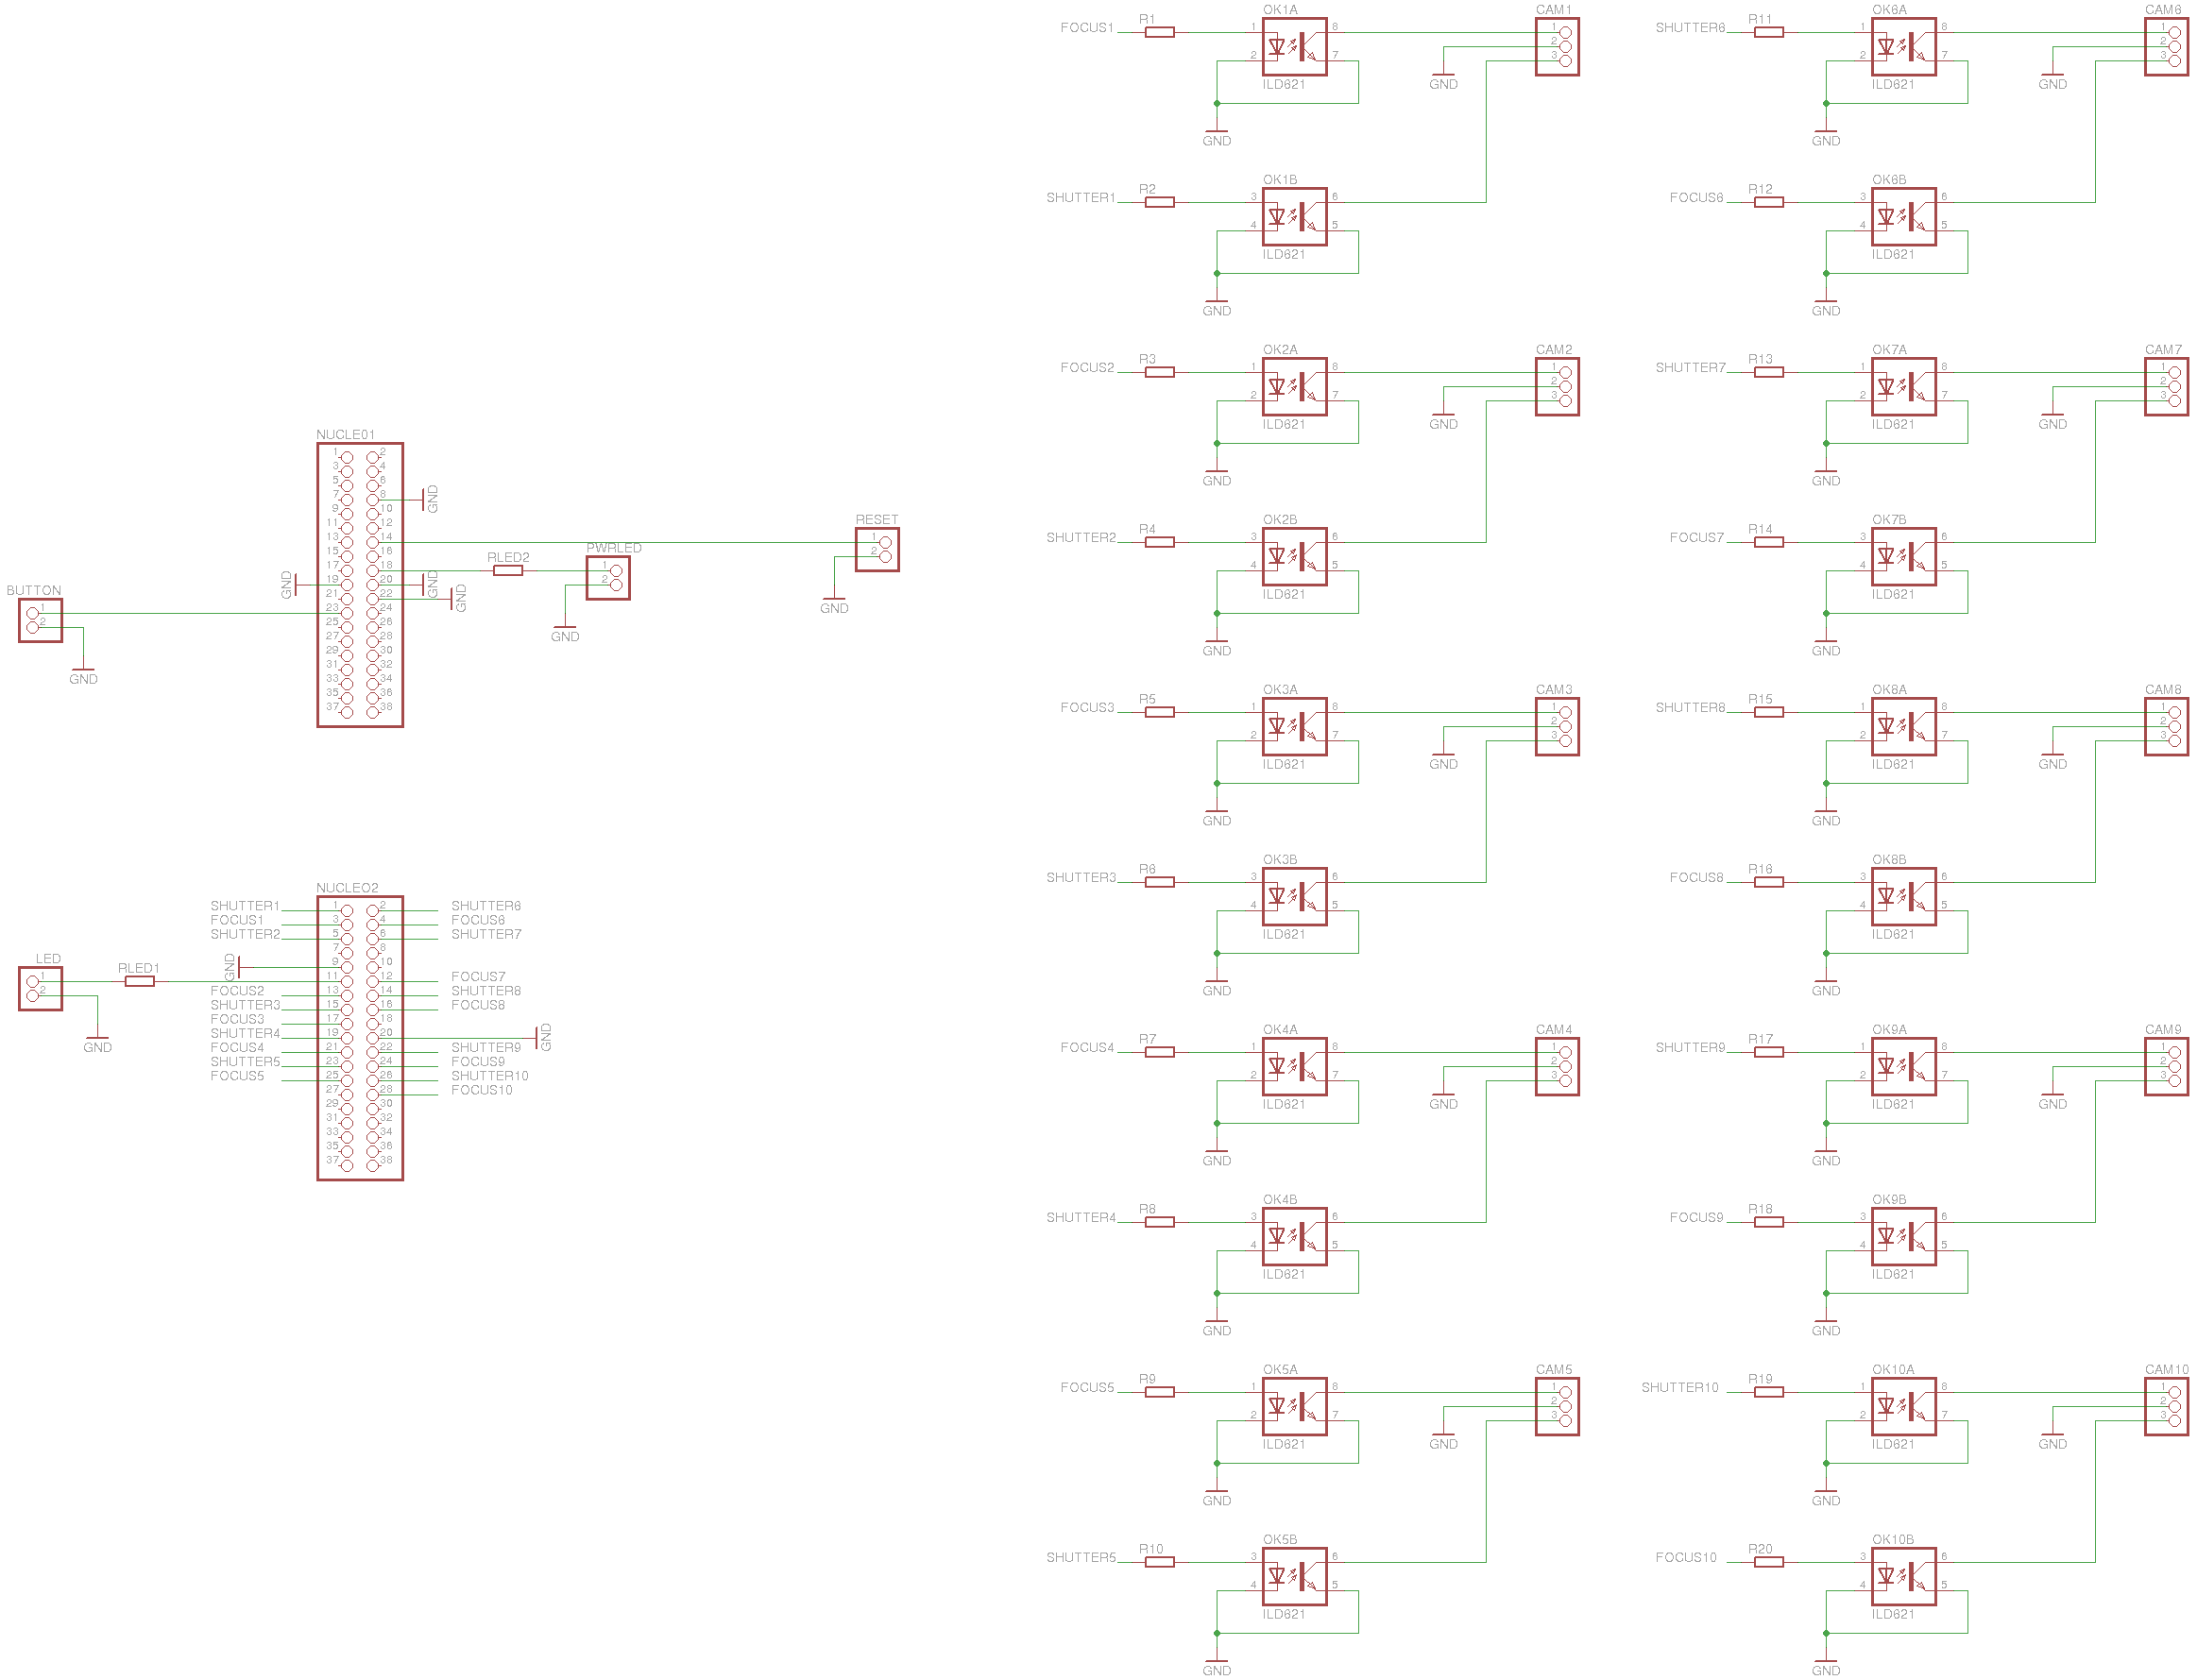
\includegraphics[height=\textwidth, angle=90]{gfx/triggerboard-sch}
}{fig:triggerboard-sch-big}
{Remote trigger schematic}

See figure \ref{fig:triggerboard-sch-big} for a complete schematic.

\subsection{Circuit board layout}

\simplefig{p}{%
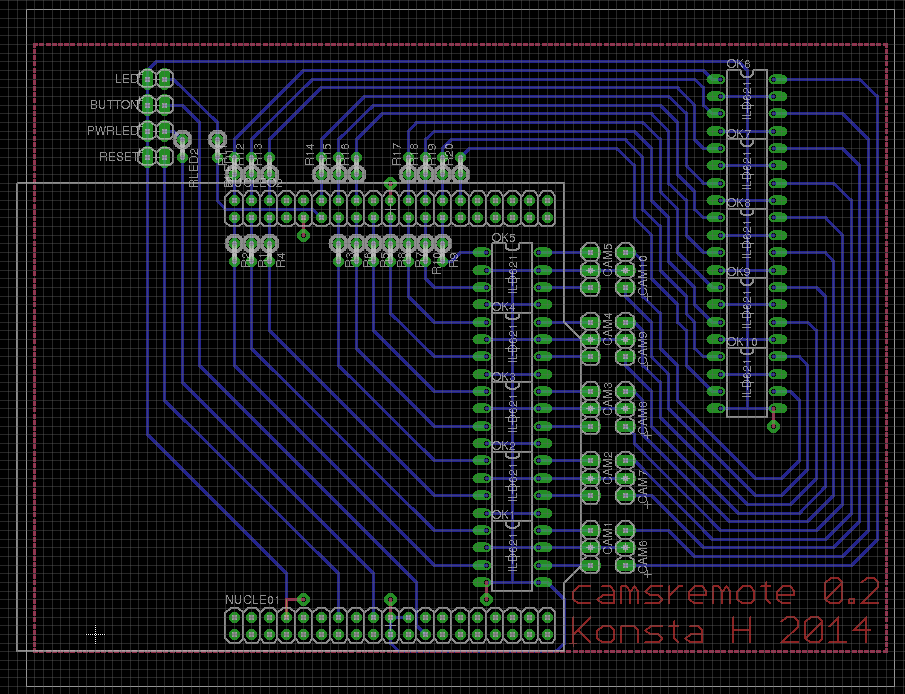
\includegraphics[height=\textwidth, angle=90]{gfx/triggerboard}
}{fig:triggerboard-brd-big}
{Remote trigger circuit board (PCB) layout}

The circuit board is 5 by 3.9 inches big and can use just one layer;
another layer is used as a ground plane, but the ground signals are routed along with the signals too.
The circuit is also simple enough to implement on e.g. a veroboard with some jumper wires.
Figure \ref{fig:triggerboard-brd-big} shows the board layout without a ground plane.

\subsection{Parts list}

\begin{itemize}
	\item ST Microelectronics Nucleo-F401RE microcontroller platform
	\item 10 x stereo 2,5 mm jack
	\item 10 x stereo 2,5mm male-male 3 meter cable
	\item 10 x TLP621-2 opto-isolator; others with similar pinout work too
	\item (usb cable, wire, buttons?)
\end{itemize}


\end{document}
